% Options for packages loaded elsewhere
\PassOptionsToPackage{unicode}{hyperref}
\PassOptionsToPackage{hyphens}{url}
%
\documentclass[
]{article}
\author{}
\date{\vspace{-2.5em}}

\usepackage{amsmath,amssymb}
\usepackage{lmodern}
\usepackage{iftex}
\ifPDFTeX
  \usepackage[T1]{fontenc}
  \usepackage[utf8]{inputenc}
  \usepackage{textcomp} % provide euro and other symbols
\else % if luatex or xetex
  \usepackage{unicode-math}
  \defaultfontfeatures{Scale=MatchLowercase}
  \defaultfontfeatures[\rmfamily]{Ligatures=TeX,Scale=1}
\fi
% Use upquote if available, for straight quotes in verbatim environments
\IfFileExists{upquote.sty}{\usepackage{upquote}}{}
\IfFileExists{microtype.sty}{% use microtype if available
  \usepackage[]{microtype}
  \UseMicrotypeSet[protrusion]{basicmath} % disable protrusion for tt fonts
}{}
\usepackage{xcolor}
\IfFileExists{xurl.sty}{\usepackage{xurl}}{} % add URL line breaks if available
\IfFileExists{bookmark.sty}{\usepackage{bookmark}}{\usepackage{hyperref}}
\hypersetup{
  hidelinks,
  pdfcreator={LaTeX via pandoc}}
\urlstyle{same} % disable monospaced font for URLs
\usepackage[margin=1in]{geometry}
\usepackage{graphicx}
\makeatletter
\def\maxwidth{\ifdim\Gin@nat@width>\linewidth\linewidth\else\Gin@nat@width\fi}
\def\maxheight{\ifdim\Gin@nat@height>\textheight\textheight\else\Gin@nat@height\fi}
\makeatother
% Scale images if necessary, so that they will not overflow the page
% margins by default, and it is still possible to overwrite the defaults
% using explicit options in \includegraphics[width, height, ...]{}
\setkeys{Gin}{width=\maxwidth,height=\maxheight,keepaspectratio}
% Set default figure placement to htbp
\makeatletter
\def\fps@figure{htbp}
\makeatother
\setlength{\emergencystretch}{3em} % prevent overfull lines
\providecommand{\tightlist}{%
  \setlength{\itemsep}{0pt}\setlength{\parskip}{0pt}}
\setcounter{secnumdepth}{5}
\newlength{\cslhangindent}
\setlength{\cslhangindent}{1.5em}
\newlength{\csllabelwidth}
\setlength{\csllabelwidth}{3em}
\newlength{\cslentryspacingunit} % times entry-spacing
\setlength{\cslentryspacingunit}{\parskip}
\newenvironment{CSLReferences}[2] % #1 hanging-ident, #2 entry spacing
 {% don't indent paragraphs
  \setlength{\parindent}{0pt}
  % turn on hanging indent if param 1 is 1
  \ifodd #1
  \let\oldpar\par
  \def\par{\hangindent=\cslhangindent\oldpar}
  \fi
  % set entry spacing
  \setlength{\parskip}{#2\cslentryspacingunit}
 }%
 {}
\usepackage{calc}
\newcommand{\CSLBlock}[1]{#1\hfill\break}
\newcommand{\CSLLeftMargin}[1]{\parbox[t]{\csllabelwidth}{#1}}
\newcommand{\CSLRightInline}[1]{\parbox[t]{\linewidth - \csllabelwidth}{#1}\break}
\newcommand{\CSLIndent}[1]{\hspace{\cslhangindent}#1}
\usepackage{amsmath}
\usepackage{booktabs}
\usepackage{multirow}
\usepackage{dcolumn}
\usepackage{lastpage}
\usepackage{fancyhdr}
\usepackage{graphicx}
\usepackage{wrapfig}
\setlength\parindent{24pt}
\usepackage[explicit]{titlesec}
\titlespacing\subsubsection{0pt}{12pt plus 4pt minus 2pt}{0pt plus 2pt minus 2pt}
\pagestyle{fancy}
\fancyhead{}
\setcounter{page}{0}
\fancyfoot[CO,CE]{Page \thepage\ of \pageref{LastPage}}
\renewcommand{\headrulewidth}{0pt}
\usepackage{floatrow}
\floatsetup[figure]{capposition=top}
\floatsetup[table]{capposition=top}
\usepackage{setspace}
\usepackage{booktabs}
\usepackage{longtable}
\usepackage{array}
\usepackage{multirow}
\usepackage{wrapfig}
\usepackage{float}
\usepackage{colortbl}
\usepackage{pdflscape}
\usepackage{tabu}
\usepackage{threeparttable}
\usepackage{threeparttablex}
\usepackage[normalem]{ulem}
\usepackage{makecell}
\usepackage{xcolor}
\ifLuaTeX
  \usepackage{selnolig}  % disable illegal ligatures
\fi

\begin{document}

\thispagestyle{empty}

\vspace{2cm}


\includegraphics[]{images/ku_logo_no_txt.png}

\vspace{2cm}

\Large

\textbf{University of Copenhagen}

\textbf{Department of Sociology}

\begin{centering}

\vspace{3cm}

\Large

\doublespacing
\textbf{MORE THAN LIKES: HOW NEWS CONTENT INFLUENCES AUDIENCE ENGAGEMENT ON SOCIAL MEDIA}

\vspace{1 cm}

\normalsize
\singlespacing
A Master Thesis by

\vspace{0.5 cm}

\Large

\textbf{Tobias Priesholm Gårdhus}

\normalsize
\vspace{0.5 cm}

\&

\vspace{0.5 cm}
\Large
\textbf{Mads Lang Sørensen}

\normalsize
\vspace{1.5 cm}

Supervisor: Christian Borch 


Number of characters: 217,328


Date: 31\textsuperscript{th} of May 2023 

\vspace{1.5 cm}

\end{centering}
\normalsize

\newpage

\onehalfspacing 

\vspace*{2cm}

\begin{center}
\includegraphics[width=0.8\linewidth]{images/midjourney_gen} \end{center}
\begin{center}
An image generated by Midjourney's image generation model using the prompt: 

\noindent
\emph{“A renaissance painting of people arguing over the content of a tabloid newspaper”.}
\end{center}

\pagebreak

\hypertarget{abstract}{%
\subsection*{Abstract}\label{abstract}}
\addcontentsline{toc}{subsection}{Abstract}

This study investigates how the content of news articles influences
audience engagement on social media. Addressing research gaps in
previous studies, which often rely on limited or biased samples and
narrow definitions of audience engagement, this study utilizes machine
learning and natural language processing techniques to analyze a
comprehensive dataset of news content shared on Facebook over a span of
nearly two years. By collaborating with Ekstra Bladet, the largest
Danish tabloid media, we are able to examine multiple different
dimensions of audience engagement encompassing information selection,
emotional responses, sharing, and conversations. Through an empirical
analysis of the influence of 11 news content characteristics on eight
audience engagement outcomes, the analysis can be summarized in three
main findings. First of all, news content characterized by
unexpectedness and soft news increases individualistic behaviors, such
as clicking on articles, while impact and hard news increase social
behaviors, such as sharing and having conversations. Secondly, the
emotional framing of news content elicits similar emotional responses
among the audience, with positivity and negativity prompting more
recognizing and offensive language, respectively, in the comment
section. Thirdly, news content related to timeliness and proximity shows
limited effects on audience engagement. These findings highlight the
multidimensional nature of audience engagement, underscoring that there
is no universal influence of news content on audience engagement on
social media.

\hypertarget{declaration-of-responsibilities}{%
\subsection*{Declaration of
Responsibilities}\label{declaration-of-responsibilities}}
\addcontentsline{toc}{subsection}{Declaration of Responsibilities}

Tobias Priesholm Gårdhus: 1, 2.1, 2.3, 2.5, 2.6, 3.2, 3.4, 3.6, 4.1,
4.3, 4.5, 5.1, 5.3, 6

\noindent Mads Lang Sørensen: 1, 2.2, 2.4, 2.6, 3.1, 3.3, 3.5, 3.6, 4,2,
4.4, 4.5, 5.2, 5.4, 6

\hypertarget{declaration-of-third-party-collaboration}{%
\subsection*{Declaration of Third-party
Collaboration}\label{declaration-of-third-party-collaboration}}
\addcontentsline{toc}{subsection}{Declaration of Third-party
Collaboration}

As part of the study, the authors collaborated with a third-party,
Ekstra Bladet, for data availability. However, no conflict of interest
has arisen throughout the process.

\pagebreak

\singlespacing

\setcounter{tocdepth}{3}
\tableofcontents

\pagebreak

\onehalfspacing 

\hypertarget{introduction}{%
\section{Introduction}\label{introduction}}

\hypertarget{background}{%
\subsection{Background}\label{background}}

News media have always played a central role in a well-functioning
democracy. The democratic role of media is to serve as an independent
and objective reporter of the truth (Herman \& Chomsky 1988:55). A
common metaphor is that the media represents the watchdog of democracy
by exposing the elite and those in power (Kovach \& Rosenstiel
2014:160ff). Furthermore, news media has an important obligation to
inform and facilitate public discussion about important societal topics
(Aalberg \& Curran 2012:3; Habermas 1999). However, in recent years, the
role of the media has been questioned due to new digital technologies
and possibilities. Perhaps the most significant consequence is the
changing relationship between media and their audiences (Richardson \&
Stanyer 2011; Livingstone 2016:2).

Increasingly, many people turn to social media as their preferred
platform for reading and engaging with news content. For the first time
in 2022, Danish audiences spent more time on social media than on
traditional print, radio, and broadcast media (DR Medieforskning
2022:14). Social media allow users to engage with news content in far
more ways than when it was distributed through newspapers, radio, or TV
(Jenkins et al.~2013:6ff). Furthermore, media organizations, editors,
and journalists no longer hold the monopoly of media production and
dissemination; anyone can participate in debates and act as a reporter
or commentator (Deuze 2005:451). In many ways, the audiences play a more
active role in the relationship with the media. Unlike the days of
opinion letters and face-to-face conversations, social media and website
analytics allow audience feedback to be tracked and analyzed directly
within the newsroom (Richardson \& Stanyer 2011; Christin 2018;
Ferrer-Conill \& Tandoc 2018:436).

The audience engagement can also be seen as a part of a digital public
sphere, where individuals discuss news content and exchange arguments.
However, this deliberative potential may not always be realized, and
some argue that the audience engagement pollutes the public debate more
than they benefit it (Papacharissi 2002). As a consequence, media
organizations have been shutting down the comment sections on their own
websites, and instead used social media platforms such as Twitter and
Facebook for social interactions (Reimer et al.~2021:4). Recently,
multiple Danish media have taken a step further and decided to remove
the possibility to comment on shared articles on their Facebook pages,
due to the number of uncivil comments. However, this decision is not
without consequences. In addition to hindering the possibility of
deliberation, these media sites' posts also reach a smaller audience --
reducing the impact of the news content (Albrecht 2022). Rather than
completely shutting down conversations around news content, it might be
more sustainable to examine what drives different kinds of audience
engagement. Following these considerations, there are democratic,
societal, and academic reasons to better understand audience engagement
with news content on social media.

\hypertarget{news-content-and-audience-engagement}{%
\subsection{News Content and Audience
Engagement}\label{news-content-and-audience-engagement}}

It is far from all kinds of news content that audiences engage with on
social media. While a minority of posts receive thousands or even
millions of clicks, likes, shares, comments, or other types of
engagements, most posts only receive a few interactions. Understanding
what drives audiences to engage or abstain from engaging with news
content on social media is important. On the one hand, audience
engagement is an important part of opinion-making, which is a central
part of a democratic society (Steensen, Ferrer-Conill \& Peters
2020:1665). On the other hand, audience engagement may also affect the
production of media content by determining what content is popular and
thus also what content is most profitable for the media (Martin 2019).
The concept of audience engagement has been defined in many different
ways, but generally it refers to an active or intentional orientation
towards the news content (Broersma 2019:1). In this study, we argue that
audience engagement should be understood as a multifaceted phenomenon
encompassing different dimensions related to information selection,
emotional reactions, sharing of content, and not least having
conversations about content.

Research has identified several factors that influence audience
engagement on social media. In a review by Kümpel et al.~(2015) three
types of factors are identified: users, content, and social networks.
This distinction is reminiscent of the classical work on media and
audiences by Katz \& Lazarsfeld (1955), where they identify five
intervening variables between media and audiences: exposure, medium,
content, predispositions, and interpersonal relations. In this study, we
will focus only on how one of these variables influence audience
engagement: the news content itself.

To determine the characteristics of news content that might influence
audience engagement, many studies have used the idea of news values.
Taxonomies of different news values have traditionally been used as a
journalistic guideline of a story's newsworthiness, but it has also been
adapted to explain how audiences evaluate the relevance of content
(Harcup \& O'Neill 2001:7; Eilders 2006). From the original formulation
by Galtung \& Ruge (1965) to contemporary reformulations of news value
theory, the categories of news values have varied greatly, but they
often include news content characteristics such as timeliness,
unexpectedness, proximity, negativity, and positivity.

\hypertarget{empirical-gap}{%
\subsection{Empirical Gap}\label{empirical-gap}}

The question of how news content influences audience engagement on
social media has been approached in various fields within both social
sciences, humanities, and natural sciences (Kümpel et al.~2015:8).
Although a lot of research has been conducted within this field, we
argue that specifically two empirical gaps remain.

First and foremost, most studies have relied on smaller samples of the
shared news content. Articles, posts, and comments have mainly been
sampled based on different analytical heuristics (e.g., selection for
qualitative analysis) or technical limitations (e.g., the
restrictiveness of social media platform's data access), while few
studies have computationally analyzed a full population of posts and
comments over an extended period. Furthermore, some studies have only
studied the news content that is most engaged with, but not what is less
engaged with (Kümpel et al.~2015:8-9). This limitation often stems from
data constraints, where empirical analyses are restricted to the top
news articles and their engagement. This approach is particularly
problematic, since it only examines what is successful and not what is
not successful. To better determine the factors driving audience
engagement, the complete population of news articles should be included
in the analysis.

A second limitation of previous research is the predominantly simple and
narrow conceptualization and measurement of audience engagement. Often,
audience engagement is aggregated into basic popularity cues, such as
the number of likes or shares (Steensen et al.~2020:1663). However,
audience engagement is a multifaceted phenomenon that can be both
behavioral and felt (Steensen et al.~2020:1665). While the felt
engagement is difficult to capture with quantitative metrics, digital
traces enable us to construct different measurements for behavior. Even
if we only consider behavioral engagement, there might be a significant
difference between a user simply clicking the link, liking a post,
sharing it to their own feed or even discussing the content in a comment
thread. While quantitative popularity cues are often the focus for media
organizations due to their connection to ad revenue, audience engagement
may also contain undesired behaviors such as incivilities in the comment
sections (Martin 2019:21; Su et al.~2018; Chen et al.~2020). To our
knowledge, no previous empirical studies have examined how different
news content might drive different dimensions of audience engagement.

\hypertarget{research-question}{%
\subsection{Research Question}\label{research-question}}

This study seeks to close the empirical gaps described in the previous
section. Overall, we seek to answer the following research question:

\begin{quote}
\emph{How does the content of news articles influence audience
engagement on social media?}
\end{quote}

\hypertarget{analytical-contribution}{%
\subsection{Analytical Contribution}\label{analytical-contribution}}

This study aims to bridge the empirical gaps in previous research on the
relation between audience engagement and news content by constructing a
unique and comprehensive dataset. The creation of our dataset and
analysis is made possible by collaborating with Ekstra Bladet - the
largest tabloid media in Denmark. Approximately one million people visit
their website every day. Ekstra Bladet also publish a printed newspaper
and share their articles on various social media such as their Facebook
page with over 400,000 followers. While tabloid in style, they cover all
areas of society and journalistic practice, ranging from celebrity
gossip to award-winning investigative journalism (Journalistforbundet
2023).

By collaborating with Ekstra Bladet, we can construct a more complete
dataset that overcomes the empirical limitations of previous research.
First of all, we are able to include all articles shared on Ekstra
Bladet's Facebook page for almost two years in our analysis. This allows
us to analyze a complete population of articles for a longer period --
rather than relying on a smaller sample that could contain biases or
lack representativeness. To be able to construct measures of audience
engagement and news content characteristics for this extensive dataset,
we apply computational methods, including machine learning and natural
language processing techniques, rather than the manual hand-labelling
that most previous studied have relied upon. Secondly, we examine social
media engagement by a multitude of different manifestations instead of
only relying on a simple and narrow measurement. Our access to Ekstra
Bladet's Facebook page allows us to retrieve detailed post and comment
data from Facebook, and therefore collect a multitude of features not
otherwise available. Instead of only retrieving common popularity cues
such as the number of likes, we are also able to collect text content
and structure of the comment section, and metrics that are only visible
to the Facebook page-owner i.e., number of clicks on the shared link. In
this way, our study extends and improves the previous empirical
foundation by both including a more complete population of news content
and a more comprehensive understanding of audience engagement on social
media.

\hypertarget{data-and-methods}{%
\subsection{Data and Methods}\label{data-and-methods}}

Our dataset is constructed by combining two different data sources. The
first dataset comes from Ekstra Bladet's database and consists of
article content and aggregated user behavior on their website. The
second dataset is collected from Facebook and consists of all posts made
by Ekstra Bladet's Facebook page, along with information about the
engagement for the posts and their comment sections. Our unit of
observation is therefore the shared posts for which we construct the
features of news content characteristics and audience engagement on
Facebook.

The dataset spans over almost two years from the 28\textsuperscript{th}
of February 2021 to the 1\textsuperscript{st} of January 2023 and
contains 18,350 Facebook posts. In aggregate metrics, our measures of
audience engagement encompass approximately 5.5 million comments, 7
million likes, and 230 million clicks on links to the shared articles.
As audience engagement is defined as a multifaceted phenomenon, we
operationalize its various dimensions on social media into eight
different outcomes related to information selection, emotional
responses, sharing, and conversations about news content. Similarly, we
define 11 news content characteristics mainly derived from news value
theory. Utilizing multiple linear regression, we analyze the influence
of these 11 news content characteristics on each of the eight
measurements of audience engagement on social media.

\hypertarget{reading-guide}{%
\subsection{Reading Guide}\label{reading-guide}}

The thesis is structured as follows. Section 2 (Theoretical Background)
delves into the existing body of knowledge surrounding audience
engagement and news content. We review relevant previous studies,
theories, and frameworks that inform our research, and highlight the two
research gaps that our study aims to address. Section 3 (Data and
Methods) describes the research design, data collection,
operationalization of audience engagement and news content, and the
analytical methods employed. The last part of Section 3 also outlines
important background information about our case of study, Ekstra Bladet.
Section 4 (Analysis) presents the results of our empirical analysis
structured in four dimensions of audience engagement on social media:
information selection, emotional responses, sharing, and conversations.
Concluding on Section 4, we present three main findings across the
outcomes of audience engagement on social media. In Section 5
(Discussion), we discuss our empirical research in the light of the
societal and theoretical implications, the reliability and validity, as
well as the generalization of our findings to other cases. Section 6
(Conclusion) summarizes the key findings of the study and highlights
limitations of the study along with suggestions for further research in
the field.

\pagebreak

\hypertarget{theoretical-background}{%
\section{Theoretical Background}\label{theoretical-background}}

In this section, we review and discuss the theoretical background and
previous literature related to our study. The research subject of our
study has been approached from multiple different disciplines within
both the humanities, natural sciences, and social sciences. In the
following theoretical and empirical review, we include related research
across different scientific approaches, while our own approach is mainly
sociological.

The first part (2.1) describes how theories of the relationship between
media and audiences have developed until today, and how they are
relevant to our study. The second part (2.2) focuses on the consequences
of social media and digital technologies and relates this digital
evolution to the relationship between media and audiences. These two
first parts serve as background information that places our study in a
broader theoretical context. Subsequently, the third part (2.3)
elaborates on the concept of audience engagement on social media and
presents findings from previous studies. In the fourth part (2.4), we
consider news content might be understood, and what characteristics of
news content might influence audience engagement. In the final part
(2.5), we discuss two empirical limitations within previous research,
which shows the relevance of our current study.

\hypertarget{media-and-audiences}{%
\subsection{Media and Audiences}\label{media-and-audiences}}

The relationship between media and audiences is an essential topic
within media and communications research (Livingstone 2016:1). The
concept of an audience has been central since the first formulations of
media theories, and in the current digital age, the concept of audiences
is more prevalent than ever (Livingstone 2016:1-2). In this section, we
will describe the theoretical developments of the theories about media
and audiences, and finally discuss how the idea of audiences has become
central to contemporary debates in media studies.

\hypertarget{mass-media-and-passive-audiences}{%
\subsubsection{Mass Media and Passive
Audiences}\label{mass-media-and-passive-audiences}}

\noindent The early formulations of theories about media are closely
related to the emergence of mass media (Merrin 2014:95). The
popularization of broadcasting through radio and television gave rise to
the concept of a mass being stimulated with content by a single media
producer (Merrin 2014:94). Lippmann (1922) was one of the first to
describe the idea of a transmission model where media is sent from the
producer to the audience. He emphasized how mass media was shaping
public opinion by transmitting cognitive stereotypes to a mass of people
(Lippmann 1922). Consequently, he was quite critical of mass media, as
it carries the potential to manipulate rather than inform the public.
This critical perspective has been continued even more famously in the
works of Herman and Chomsky and their idea of manufacturing consent
(Herman \& Chomsky 1988), as well as in the works of Adorno and
Horkheimer on enlightenment as mass deception (Adorno \& Horkheimer
2002; Adorno 1991). In both of these approaches, the mass audience is
deceived, as the media present them with simplified or biased portrayals
of the world, promoting conformity rather than an informed and critical
consciousness (Adorno 1991:104).

The concept of a transmission model of media has also been developed
within a tradition that is less normative, adopting a more positivistic
approach. Prominently, the two mathematicians Shannon and Weaver (1949)
summarized the relationship between media and audiences in their
sender-message-receiver model. This theoretical model has a clear causal
relationship: a sender (e.g., the news media) transmits a message, which
is received by the audience and produces a specific effect. Similar to
Shannon and Weaver's model, Lasswell (2007) also described a
transmission model formulated as a chain of questions: who says what in
which channel to whom with what effect (Wanta \& Myslik 2019:59-60)?
These theoretical models have had a large impact on media studies, and
many studies have examined media effects of different kinds of content
and audiences, but always with an emphasis on a one-way, causal
direction from media producers to media consumers (Wanta \& Myslik
2019:59-60).

\hypertarget{the-idea-of-active-audiences}{%
\subsubsection{The Idea of Active
Audiences}\label{the-idea-of-active-audiences}}

\noindent Most contemporary research within media studies has moved away
from the notion of audiences as passive masses without any agency. In
the latter half of the 20th century, several different approaches
contested the previous understanding of audiences. Different theoretical
approaches have argued that audiences should be seen as being more
diverse and having more agency. Three of the most important approaches
that we will mention here are: 1) interpersonal relations by Katz \&
Lazarsfeld (1955), 2) the encoding-decoding model by Hall (1973), and 3)
Livingstone's (2005) concept of active audiences.

Katz and Lazarsfeld (1955) were among the first to challenge the
mass-communication-idea of audiences as a passive receiver. They
identify five different intervening variables affecting the relationship
between media and audiences: exposure level, medium type, media content,
audience predispositions, and interpersonal relations (Katz \&
Lazarsfeld 1955:20-25). Their work emphasizes the fifth variable,
interpersonal relations, since it gives a new kind of agency among the
audience members. Readers of a newspaper and viewers of a television
shows are not just separate individuals, but they have interpersonal
relationships through social networks and group norms, which mediates
the influence of the media (Katz and Lazarsfeld 1955:43-44). Katz and
Lazarsfeld also introduced the idea of a two-step flow of communication,
where opinion leaders -- people with especially significant
interpersonal influence -- distribute and mediate the flow of
information from media to the audiences (Katz \& Lazarsfeld 1955:32).

Another important contribution within media studies is the works of Hall
(1973). He argues that there can never be one single stimuli-effect of a
media message, because both the process of media production and media
reception are embedded in ideologies (Hall 1973:265). When journalists
and media workers produce content, it is encoded with different
knowledge and assumptions, and subsequently the media content is decoded
by the audience and reacted to according to their structural and
cultural position.

In more contemporary research, the idea of active audiences has also
been greatly emphasized by Livingstone (2006:9). She argues that
audiences are increasingly diversified and situated within specific
communities (Livingstone 2006:9-10). This perspective strongly
emphasizes that media messages are fully interpreted within communities,
and thus the approach has had a strong focus on ethnographic methods
(Livingstone \& Das 2013:1-2). In its most extreme formulation, there is
no inherited meaning in media content, and media content will have
completely different meanings for different communities (Philo et
al.~2015:464).

Although the approaches of Katz and Lazarsfeld, Hall, and Livingstone
are quite different in nature, they all share the common trait of
imagining an audience that has some kind of agency -- both towards media
producers and each other. To some extent, the theoretical approaches to
media and audiences can be placed on an axis of how much agency is
attributed to the audience, and how unified or fragmented the audience
is thought to be (Philo et al.~2015:464). While recognizing that these
underlying dynamics are a part of the subject, our study will have a
specific empirical focus on the relationship between the news content
and audience engagement.

\hypertarget{audiences-2.0}{%
\subsubsection{Audiences 2.0}\label{audiences-2.0}}

\noindent The idea of an audience is both a central pillar in media
theory and an essential part of everyday practices in newsrooms
(Livingstone 2016:1-2). Nevertheless, many researchers have started to
question the contemporary relevance of the concept of audiences. The
critique is mainly a consequence of the concept being firmly connected
to specific technological mediums: mass broadcasting media such as radio
and television (Livingstone 2016:2). Recently, mass broadcasting media
has been greatly challenged by digital media. Some argue that this
technological evolution also has deep consequences for previous media
theories - because they simply no longer fit the digital reality - to
such a degree that we need to develop a media studies 2.0 (Merrin 2014).

While it seems exaggerated to discard decades of media studies, there is
no doubt that the digital technological advancements have introduced new
possibilities for the media ecology and not least for the relationship
between media and audiences. Where traditional mass media is
characterized by a one-to-many-relationship, digital media allows for a
many-to-many-relationship (Livingstone 2016:2). On the internet, anyone
can produce content that resembles journalistic content. This basic
access to publishing challenges one of the most rudimentary principles
of traditional journalism: that the journalist is the gatekeeper of
producing, selecting, and exposing content to the audience, which
passively consumes it (Deuze 2005:451). While there is a possibility for
everyone to take up the job as a journalist, it remains questionable if
everyone actually does involve themselves in producing content
(Livingstone 2016:2). With technological breakthroughs, there is a
tendency make overly enthusiastic proclamations of an entirely new era,
but we have yet to see the distinction between news content producers
and news content consumers completely vanish (Webster 2014:2;
Livingstone 2016:2).

\hypertarget{subconclusion-media-and-audiences}{%
\subsubsection{Subconclusion: Media and
Audiences}\label{subconclusion-media-and-audiences}}

\noindent This first part of the theoretical background outlines how the
concept of audiences has been central to the interdisciplinary field of
media studies. Today, most theories of audiences and media regard the
audiences as active and diverse communities. The concept of audiences is
even more emphasized and discussed with the invention of new, digital
media, where audiences have even more agency. Our study continues in the
line of research that understands audiences as active and participating
by examining audience engagement behavior with news content on social
media.

\hypertarget{digital-media}{%
\subsection{Digital Media}\label{digital-media}}

In the previous section, we consider how the evolution of digital
technologies and especially social media have had significant
consequences for the relationship between media and their audiences. In
this section, we describe these new digital technologies and news media
in a broader sociological context. Lastly, we discuss previous research
of the social media, Facebook, which is the specific focus of our study.

\hypertarget{digital-trace-data}{%
\subsubsection{Digital Trace Data}\label{digital-trace-data}}

\noindent When researchers refer to the digital age or the evolution of
digital technologies in the 21\textsuperscript{st} century, the concrete
technological inventions often concern the exponential increase in
computational power and storage capacity (Salganik 2018:3-4). Every
second, massive amounts of data are written to huge databases. Included
in this stream of data is especially the monitoring of our digital and
digitalized behavior -- commonly named digital trace data. Digital trace
data has several advantages. First of all, they are big i.e., they exist
in large quantities (Salganik 2018:17). Furthermore, they are found data
meaning that it is real, digital or digitized behavioral data, and
therefore also non-reactive to the collection by the researcher
(Salganik 2018:24). There are also some disadvantages of using digital
trace data. These disadvantages are that digital trace data can be
noisy, algorithmically confounded, or incomplete -- meaning that
relevant features such as background information of the users might not
be available (Salganik 2018:35ff). The concept of big data has also been
used to describe the accumulation and analysis of digital trace data.
However, this term is often used in a variety of ways with no clear
singular definition (Sætnan et al.~2018:6).

In the context of news and media, the evolution of digital trace data
has also had a huge impact. In the literature, several studies have
examined how audience analytics mainly based on these digital trace data
have made its way into the newsrooms (Christin 2018; Ferrer-Conill \&
Tandoc 2018). The implementation of different analytics services and
dashboards in the everyday of the journalists, editors, or even specific
audience editors have been commonplace in many different media
organizations (Ferrer-Conill \& Tandoc 2018). Digital trace data and
predictive modelling have become especially valuable for media
organizations, since it is related to recommendation of advertisements,
which is a major source of income for most modern media organizations
(Martin 2019:21). Moreover, as the study by Christin (2018) of an
American and a French newsroom have shown, digital trace data can be
interpreted and used quite differently within media organizations
(Christin 2018). The constant interpretation of performance metrics
might cause a reactivity among journalists where they adapt their work
as they become aware that they are being evaluated of their work
(Christin 2018:1386; Espeland \& Sauder 2007:1). In this way, the
introduction of quantitative feedback based on the digital trace data
can have both good and bad consequences, both in terms of making content
more relevant to the audience, but it could also decrease the kind of
news that are important but might not be among the most popular
(Christin 2018:1409). While these studies focus on the effect on
audience engagement on the media production, our study focuses on what
precedes these evaluations: the measurement of how audiences engage with
different news content.

\hypertarget{social-media}{%
\subsubsection{Social Media}\label{social-media}}

\noindent In addition to the technical evolution of the capacities of
computers, a significant newcoming in the 21st century has been the
invention and popularization of social media or social network sites.
Social media has many different definitions, but a common trait is that
it is a digital service that connects people (Aichner et al.~2021:220).
Thus, social media is different from previous media, because it is
social -- it is many-to-many communication rather than one-to-many mass
communication (Livingstone 2016:2). Previous research has identified
different uses of social media such as socializing with friends or
family, romance and flirting, job seeking or networking, and other kinds
of interaction with strangers, organizations, companies, content and
much more. The many uses of social media highlight how many different
social phenomena have been digitalized or amplified by the invention of
social media (Aichner et al.~2021:220).

A lot of research has been devoted to the study of social media, and a
few areas of research stand out as particularly prevalent. This is
especially evident for the phenomenon of social and political
polarization, which has garnered significant attention in social media
research. Polarization refers to a division between different groups of
people or sets of opinions, and the research area is closely connected
to related concepts such as echo chambers or filter bubbles that both
refer to a social homophily of ideologies, i.e., that you only interact
with other people, who have the same opinions as yourself (Bail 2021). A
lot of studies have examined the prevalence of polarization of social
media, as it has been hypothesized that political polarization is
increased on social media. For example, Bail et al.~(2018) find that
Twitter users being exposed by statements of the opposite republican or
liberal ideology become more extreme in their respective political
ideology. In general, they find that users become less moderate in their
opinion by being on social media and being exposed to different
political statements (Bail et al.~2018; Bail 2021). However, the
popularized concepts of echo chambers and filter bubbles have been quite
contested, as they represent a too simplified description of the
informational exchanges on social media (Bail 2021). For example, a
study by Gentzkow and Shapiro (2011) found that the polarization of
engagement with news media on social media is lower compared to offline
media engagement such as newspaper subscriptions. Thus, polarization
might be a problem, but the idea of social media amplifying polarization
seems to be more complex than first anticipated. Similarly, Bakshy et
al.~(2015) found that individual selection when engaging with media
content on social media leads to more polarization than the algorithmic
sorting of the media content. Another interesting study is Schmidt et
al.~(2017), who finds that more active users tend to focus on a small
number of news sources in their social media feed. Rather than
constructing personalized filter bubbles of news content, current
research suggests that the social media platform tend to homogenize the
news content exposure, so that a small number of news media gain most of
the exposure and engagement on social media (Nechushtai et
al.~2023:18-19).

Another area of research within social media and news is the impact of
misinformation, disinformation and fake news. The increase of
misinformation and fake news is often related to polarization as studies
have shown how strong political partisanship might drive believing in
factual incorrect media content (Bail 2021:109). Previous research has
examined how adding warning tags or correction statements might
influence the effect of misinformation, but the studies are not in
agreement (Muhammad \& Mathew 2022:279). Some studies have found that
warnings can reduce the spread of misinformation, while other have
suggested a backfire-effect -- a cognitive confirmation bias, where
corrections of misinformation increase the belief in the incorrect
information (Nyhan \& Reifler 2010; Wood \& Porter 2019).

There are many different social media with different specific
functionalities, norms and likely also different types of people using
them. Currently, social media such as Instagram, Snapchat and TikTok are
most popular among younger people, while a social media like LinkedIn is
more popular among those with higher levels of education (Auxier \&
Anderson 2021). The popularity of social media can change quickly, and
previous popular sites such as Myspace or Google+ have completely
disappeared from the landscape of social media. However, in most
countries Facebook remains the most popular and widely used social media
(Auxier \& Anderson 2021; DR Medieforskning 2022:13; Ortiz-Ospina 2019).

\hypertarget{facebook}{%
\subsubsection{Facebook}\label{facebook}}

\noindent Across the world, Facebook remains the most popular social
media with close to 3 billion daily active users (Meta 2022). In
Denmark, 65\% of the population use Facebook on a daily basis (DR
Medieforskning 2022:13). According to Facebook itself, the mission of
the company is \emph{``Giving people the power to build community and
bring the world closer together''} (Meta 2023). To a certain extent, the
company's slogan reflects that Facebook have always been a site for
managing your social network, and previous research have also shown that
the primary uses for joining Facebook are social interaction and social
identity-building (Caers et al.~2013:984-985). However, Facebook and
especially the company behind Facebook, Meta, have over time developed
into an overarching platform by co-integrating with Meta's many other
social media and digital services such as Messenger, Instagram, WhatsApp
(Helmond et al.~2019). Similar with most other social media, the
financial model for Facebook is based on using digital trace data of the
users to sell advertisements to over 90 million businesses around the
world (Helmond et al.~2019).

Engagement with media and news content is also a vital part of using
Facebook. In a Danish context, Facebook is the largest source of news
content exposure compared to other social media (DR Medieforskning
2018:48). Especially for young people between 15 and 24 years old,
Facebook serves as the primary source for news content (DR
Medieforskning 2018:48). However, the relationship between Facebook and
media organizations has been complicated. The most significant dispute
between Facebook and news media was when the Australian government in
2019 tried to force Facebook to pay media organizations for showing
their news content, and Facebook reacted by removing all news content
for Australian users (Leaver 2021). While an agreement was eventually
reached and Australian news content was reinstated on the Facebook
platform, this incident highlighted the dual role of Facebook as both a
distribution platform for news content exposure and a potential risk to
the business models of media organizations. News organizations often
share their content on Facebook, but the underlying goal is commonly to
use social media engagement to direct potential audiences away from
Facebook and onto their respective websites (Humprecht et al.~2020:1).

\hypertarget{subconclusion-digital-media}{%
\subsubsection{Subconclusion: Digital
Media}\label{subconclusion-digital-media}}

\noindent This second part of the theoretical background describes how
digital technologies and the invention of social media has had a
significant impact on news media and their audiences. Extensive research
has been dedicated to studying social media, where a particular focus
has been on areas such as polarization and misinformation. Lastly, the
relationship between audiences and news media is especially interesting
on Facebook, as this social media is the largest and for many serves as
a central source of engaging with news content.

\hypertarget{the-many-faces-of-audience-engagement}{%
\subsection{The Many Faces of Audience
Engagement}\label{the-many-faces-of-audience-engagement}}

In previous research, the idea of audience engagement has been defined
and measured in many different ways. When studying audience engagement
on social media, measurements of audience engagement have been
everything from reading the news content, liking the post, sharing the
article, commenting on the post, and not least the content and tone of
the conversations around the article. In the following section, we will
discuss how audience engagement can be defined, and how we may think of
it as a multifaceted phenomenon in which different kinds of behaviors
relate to different kinds of motivations for engaging with the news
content.

\hypertarget{what-is-engagement}{%
\subsubsection{What is Engagement?}\label{what-is-engagement}}

\noindent The concept of audience engagement is growing in popularity
within both academia and media organizations, and it has become almost a
media industry buzzword (Nelson 2021:2350-2351; Lawrence et al.~2018).
In some newsrooms, there are job descriptions focusing on audience
engagement, and there is a growing industry of audience engagement
services and tools offered to journalists and media organizations
(Nelson 2021:2351). However, there is often a lack of concrete
theoretical definitions of what engagement actually entails (Steensen et
al.~2020:1664).

One very broad definition of engagement is that it \emph{``refers to the
cognitive, emotional, or affective experiences that users have with
media content or brands``} (Broersma 2019:1). The main component of this
definition is that engagement is different from simply exposure -- it
\emph{``denotes an active and intentional orientation toward what users
read, view, or hear.''} (Broersma 2019:1). However, this is still a
quite open and perhaps unprecise definition of engagement (Steensen et
al.~2020:1664). Some research additionally distinguishes between felt
and behavioral engagement, where felt engagement refers to affective and
cognitive reactions, and behavioral engagement means practices that can
be observed (Steensen et al.~2020:1665). Thus, felt engagement could be
having angry or happy feelings about content or changing attitudes as a
result of content, while behavioral engagement could be reading a news
article, liking content on social media, sharing news content, or
writing comments.

In both academia and media organizations, there have been an emphasis on
behavioral engagement, because it is easier to measure and quantify, and
behavioral engagement might also be used as a proxy for felt engagement
(Steensen et al.~2020:1665). However, even if only behavioral engagement
is considered, we argue that there are substantial differences in what
the different audience engagement behaviors represent. In their review
on definitions of audience engagement, Gajardo and Meijer (2022) argue
that previous research has predominantly concentrated on attention and
time spent on news content, while less consideration has been given to
how the time is spent or the quality of the engagement. They highlight
audience engagement as a complex and multifaceted phenomenon composed of
different dimensions of behaviors and emotional orientations (Gajardo \&
Meijer 2022; Steensen et al.~2020). In the following, we will further
elaborate how different audience engagement behaviors might relate to
various underlying motivations.

\hypertarget{motivations-for-engagement}{%
\subsubsection{Motivations for
Engagement}\label{motivations-for-engagement}}

\noindent To understand different audience engagement behaviors, we
argue that it is important to consider what motivation lies behind.
Multiple studies have found that different behaviors such as liking,
sharing, or commenting are related to different user motivations
(Almoqbel et al.~2019; Kim \& Yang 2017). In fact, there is a
theoretical approach within media studies that emphasizes how different
kinds of media uses are related to different kinds of gratifications,
i.e., different sociological or psychological motivations (Ruggiero
2000). Here, the question of what constitutes engagement is not only the
study of the kind or extent of engagement, but also what precedes or
motivates the actual action of engagement.

The theory of uses and gratifications has been described in many ways,
but originates from the work of Katz and Lazarsfeld (See Section 2.1.2).
One particular sociological formulation is the theory by Levy and
Windahl (1984), who stresses that gratifications should not be
understood as the audience being superrational and selective (Ruggiero
2000:8; Levy \& Windahl 1984:52ff). Levy and Windahl developed a
taxonomy in which audience engagement can be placed within both the
audience motivation and the phase of exposure: pre-, under-, or
post-exposure of the news content. In this way, one kind of audience
engagement might be related to a selective orientation, which happens
pre-exposure of the news content. Other kinds of audience engagement
such as discussing the news content is oriented towards socializing, and
it happens after the exposure of the news content. In this way, they
provide a theoretical example of how different kinds of audience
engagement might be explained and related to different kinds of
motivations.

The uses and gratifications approach might be particularly relevant in
the case of audience engagement on social media, as this new form of
media makes possible an increased agency of the audiences (Ruggiero
2000:20) (See also section 2.1.3). In line with this, a study by
Springer et al.~(2015) applies the approach to audience engagement on
social media - specifically the behaviors of commenting and reading
comments. They identify four dimensions of audience engagement, which
relate to different underlying motivations. These dimensions include
cognition, entertainment, social-integration, and personal identity, and
they divide user behavior into commenting (e.g., commenting) and lurking
(e.g., reading) behavior (Springer et al.~2015:800ff). Similarly, a
review by Kümpel et al.~(2015) identifies three broad motivations for
online news sharing behavior: self-serving motives like promoting
reputation or gaining social status, socializing and discussing ideas,
and altruistic motives of information sharing or seeking (Kümpel et
al.~2015:6).

As these studies exemplify, there is not a finite taxonomy or theory of
the possible uses and gratifications. Furthermore, the different
dimensions of audience engagement behaviors and gratifications might
also vary between different empirical cases (Levy and Windahl 1984:57;
Haradakis \& Humphries 2019). Although focusing on different kinds of
audience engagement behavior, both Springer et al.~(2015) and Kümpel et
al.~(2015) discuss gratifications that relate to information seeking,
socializing, and self-expression. In relation to our present study, the
idea of uses and gratifications serves as a theoretical basis for
considering how audience engagement might consist of multiple different
dimensions. The reviewed studies use the concepts of motivations and
gratifications interchangeably. In our case, we chose to mainly focus on
motivations moving forward, as it denotes the desire for an outcome. In
our study, the underlying motivations cannot be observed directly, but
we only examine behavioral outcomes. In the next four sections, we will
further examine which dimensions of audience engagement on social media
might exist -- focusing on information selection, emotional responses,
sharing content, and finally conversations and deliberation -- while
tying them to other relevant sociological theories.

\hypertarget{information-selection}{%
\subsubsection{Information Selection}\label{information-selection}}

\noindent The most basic form of audience engagement on social media
might be to simply expose oneself to the news content. In other words,
audience engagement can be to read, view, or listen to news content.
There can be many different reasons for choosing to click on a link to
an article and read it, but one of them might be to get information or
gain knowledge about the content in the article (Kormelink \& Meijer
2018). For example, it has been shown how use of media content is
related to a greater knowledge of political and current events
(Oeldorf-Hirsch 2018:227). The idea that news media play an important
role in supplying information to citizens has especially been emphasized
in the context of political knowledge as a way of maintaining an
informed democracy (Aalberg \& Curran 2012:3). It is often emphasized
how news media have an obligation to inform citizens to make decisions
based on knowledge rather than ignorance or misinformation (Aalberg \&
Curran 2012:3). However, there might also be differences in the way
information and knowledge is obtained from the media. As Eveland (2001)
has emphasized with his theory of cognitive mediation, the relationship
between exposure to news content and information gain is mediated by a
number of motivations about learning from the news (Eveland
2001:574-575). For example, a study by Eveland \& Scheufele (2000) found
that current affairs knowledge gaps between higher and lower education
groups are smaller for users that more frequently read news content.
Thus, different users might gain different amounts of knowledge from
news content (Ohme 2020). The specific question of retrieving factual
knowledge from news content from social media is also relevant in
relation to the discussion about misinformation or particular forms of
fake news on social (See also Section 2.2.2).

Particularly in the context of engaging with news content on social
media, research has discussed whether social media has a paradoxical
role for the diffusion of information from news content. On the one
hand, the extensive amount of information available creates a broad
selection of news content for the user to select and choose to read, but
on the other hand, the increased amount of available content might also
result in an information overload (Pentina \& Tarafdar 2014). Gaining
information and knowledge from news content is likely not a linear
process, but a complex mechanism of news content contributing to
sense-making and information-processing (Pentina \& Tarafdar 2014:220).

\hypertarget{emotional-responses}{%
\subsubsection{Emotional Responses}\label{emotional-responses}}

\noindent Audiences do not just use news content to get information or
knowledge. Another important part of engaging with news content is also
the phase where the content is interpreted and a form of reaction to the
content might happen (Levy and Windahl 1984:54). As described in Section
2.1.2., Hall is well-known for his ideas about this process of decoding
news content (and encoding news content for the journalists and
editors). In the process of decoding news content, Hall argued that
audiences might respond with either a hegemonic, negotiated, or
oppositional position towards the content. Quite simplified, audiences
might respond in agreement, partly in agreement, or in disagreement with
the news content exposed to them.

Another related line of research has also examined the decoding process
in relation to the emotions or feelings that might appear in audiences
in relation to certain types of news content. The study of audience
emotional reactions has been studied across diverse fields such as
psychology, neuroscience, anthropology, and sociology (Dafonte Gómez
2018:2142). An emotional reaction based on exposure to news content is
often characterized as different feelings such as anger, sadness,
positivity, hope, or happiness (Dafonte Gómez 2018:2143). A related line
of research has discussed the idea of emotional contagion, i.e., that
emotional states of persons interacting with each other tend to
influence each other towards the same emotional state (Hatfield et
al.~2014:109). Although emotional contagion is widely used within
psychology, the idea of interpersonal contagion or imitation is also a
classic sociological concept originating from the work of Tarde (Tarde
1903; Katz 2006). The idea of emotional contagion has also been
developed to include that the emotional responses of audiences tend to
converge towards the emotional framing of news content that they engage
with (Bösch et al.~2018). A study by Facebook has examined emotional
contagion on their platform to see if the emotionality of the content on
users' feed affects the emotionality of the users (Kramer et al.~2014).
They found clear evidence that the proportion of exposure to positive or
negative expressions influences the amount of positive or negative posts
that the users produced correspondingly. It is important to note that
the mentioned Facebook study has been heavily criticized as unethical
(Salganik 2018:284; Sellinger \& Hartzog 2016).

In the context of audience engagement as emotional responses on social
media, Facebook have often been the focus of study, as they in 2016
introduced an option to react to content with a number of different
emotions beyond the original like reaction (de León \& Trilling 2021:1;
Meta 2016). With this technological addition, it became possible to
materialize the emotionality through digital manifestations on each
Facebook post. Some studies have collapsed the total amount of reactions
as a general measure of valence, others have grouped the reactions into
groups of positive or negative emotions, while still others argue that
they might best be understood as a discrete set of emotional reactions
(de León \& Trilling 2021:2; Heidenreich et al.~2022).

\hypertarget{sharing-is-caring}{%
\subsubsection{Sharing is Caring}\label{sharing-is-caring}}

\noindent Long before the invention of social media, Katz and Lazarsfeld
described the importance of interpersonal relations and social ties in
the audience engagement of news content (Katz \& Lazarsfeld 1955:43-44;
see Section 2.1.2.). Interpersonal social ties can be mediating in terms
of increased exposure of content, but also conformity to social group
norms is an influential factor (Katz \& Lazarsfeld 1955:52). While
sharing of news may serve as a way of spreading information or gaining
further information, it may also be rooted in motivations of social
status-seeking or social acceptance (Katz \& Lazarsfeld 1955; Kümpel et
al.~2015:6).

In recent studies with a focus on news sharing on social media, the
intention of self-representation or group-identification has been
re-examined (Kümpel et al.~2015:6). In a study by Ihm and Kim (2018)
based on survey data, they find that individuals with a high motivation
for self-presentation are more likely to share news online across both
private messaging and public social network sites (Ihm \& Kim 2018).
Similarly, a study by Thompson et al.~(2020) has shown that the
perceived credibility of news media is related to the willingness to
share content, as sharing low-credibility news content might be damaging
to the social status of the individual.

Another perspective on sharing may be to interpret it as a form of
gift-giving to maintain social cohesion (Duffy \& Ling 2020). The idea
of gift-giving is a classical sociological theory dating back to Mauss
(2004) in which sharing or giving content is a way of establishing and
reproducing social ties. Inspired by Mauss' idea of gift-giving, Duffy
\& Ling propose the concept of phatic news sharing, that is engagement
with news content that is not directed at having longer conversation or
the information in the content, but the mere act of activating and
maintaining a social connection (Duffy \& Ling 2020:83).

In this way, there might also be different motivations for sharing news
content. The first kind of sharing described by Ihm \& Kim (2018) and
Kümpel et al.~(2015) relates to broader social status-seeking and
self-presentation, while the phatic news sharing described by Duffy \&
Ling (2020) relates to maintaining social ties between specific
individuals.

\hypertarget{conversations-and-deliberation}{%
\subsubsection{Conversations and
Deliberation}\label{conversations-and-deliberation}}

\noindent A final dimension of audience engagement is how audiences can
engage with news content by having conversations about the content. A
growing literature has examined audience engagement as conversations and
discussions in the comment sections on social media (Reimer et
al.~2021:11). These studies take different theoretical and
methodological approaches, ranging from discussions of Habermas'
theories to predictive studies of uncivil language. In the following, we
present the most important positions from this range, and the related
empirical findings that are connected to our area of research.

The research of conversations around news content often takes
inspiration from classic theoretical ideas about deliberative democracy
-- especially the work of Habermas. For media studies and especially
sociology, Habermas' theory of deliberative democracy stands as a
seminal concept when considering communicative practices. He argues that
an open, free, and independent public sphere is essential for a
well-functioning liberal democracy. Deliberative democracy is achieved
through discussions based on communicative rationality as a form of
communication where different viewpoints can be encountered and
challenged free of coercion and strategic motives (Habermas 1999). While
other forms of communication exist, deliberation is the form of
communication that the public sphere should facilitate in a
well-functioning society (Habermas 1999; Habermas 2001). Habermas'
conception of deliberative communication can be understood as a form of
democratic communication that prioritizes inclusivity, rationality, and
mutual understanding. Habermas emphasized how the media plays a crucial
role in facilitating and providing a platform for public discourse.
However, he also recognized the potential pitfalls of the media, such as
the potential for media organizations to prioritize profit over the
public interest (Wessler 2018:58).

Since the early formulation of deliberative democracy, society and
technology have developed along with the institutional and technological
situation of the public sphere (Habermas 2006, 2022). This has prompted
many researchers to reflect on and investigate the potential and
challenges of digital platforms for successful deliberation, and how
Habermas' theory of deliberation could be applied or translated to this
new reality. Ideally, the internet helps to fulfill deliberative ideals,
which can be realized through its openness and reach -- in contrast to
physical spaces' locality and traditional media's closedness. As such,
it is argued that social websites, as a public sphere 2.0, have the
potential to realize deliberative ideals in a new and improved
egalitarian context (Ruiz et al.~2011). However, it is not naturally
given that these digital technologies will realize this potential. As
Papacharissi (2002) argues, there are serious concerns which are
challenging the success of the virtual public sphere such as
polarization, dependency on big tech companies, and not least the
quality of online, political discussions (Papacharissi 2002:20).

Drawing on this theoretical foundation, many studies have sought to
empirically analyze the deliberative quality of conversations on digital
or social media. However, there has not yet been established a coherent
approach to empirically measure deliberation, and many different
operationalizations have been used (Esau et al.~2017:332). One
particular approach that has been developed especially for social media
is Esau et al.~(2017), who measure deliberative quality by four
dimensions: rationality, reciprocity, respect, and constructiveness. In
practice, rationality can be whether the discussion is on-topic, and
reciprocity relates to the depth of the conversation, e.g., if a comment
addresses another comment. The dimension of respect refers to the
absence of aggressive or offensive language, while constructiveness
captures whether comments contain proposals for solutions or similar
(Esau et al.~2017:332).

Other studies have predominantly focused on single indicators of lack of
deliberation, such as the respect dimension as a presence of uncivil
language and paid less attention to the positive indicators such as
constructiveness (Reimer et al.~2021:20f). Specifically, a large body of
research has tried to explain what factors influence the amount of
incivility in online conversations about news content. For example, Coe
et al.~(2014) found that uncivil comments increase when weightier topics
are discussed. Additionally, Diakopoulos and Naaman (2011) and Gardiner
(2018) found that topics related to politics, society, crime and
justice, disasters and accidents, the environment, and feminism are more
strongly associated with uncivil discourse. The sources cited in an
article can also influence comment civility (Coe et al.~2014). Anonymity
has a negative effect on civility and comment quality (Fredheim et
al.~2015; Santana 2014), and female journalists are particularly
targeted with hateful comments (Gardiner 2018). Furthermore, research
have also shown that the dynamics of uncivil conversations on social
media varies from cultural contexts e.g., between different countries
(Humprecht et al.~2020). Different research has also examined the
consequences of uncivil conversations for news media and results
indicate that audience's perception of news bias and credibility are
affected by the content of the comment sections, by enhancing
perceptions of bias and diminishing perceptions of favorability (Houston
et al.~2021; Kümpel \& Springer 2016; Gearhart et al.~2022).

\hypertarget{subconclusion-the-many-faces-of-audience-engagement}{%
\subsubsection{Subconclusion: The Many Faces of Audience
Engagement}\label{subconclusion-the-many-faces-of-audience-engagement}}

\noindent In this third part of the theoretical background, we discuss
the definition of audience engagement as well as related research on the
topic. In this study, we employ a broad understanding of audience
engagement as any active and intentional orientation towards news
content. Inspired by the uses and gratifications approach and a broader
literature review, we understand audience engagement on social media
through several dimensions manifested in different behaviors. Here, the
dimensions identified are behaviors related to: 1) information
selection, 2) emotional responses towards the content, 3) sharing
content either for social status or maintenance of social ties, and 4)
having conversations about the content.

\hypertarget{engaging-with-news-content}{%
\subsection{Engaging with News
Content}\label{engaging-with-news-content}}

The previous sections outline how we understand audience engagement on
social media such as Facebook. Audience engagement is a multifaceted
phenomenon, and there might also be multiple factors that influence how
audience engagement unfolds. As described in Section 2.1.2., everything
from exposure, type of medium, audience predispositions, interpersonal
relations as well as the news content itself might influence how
audiences choose to engage with the content. In this study, we chose to
focus on the last factor: the influence of the news content itself. In
this section, we will review how news content might be characterized,
and which features of news content that might influence audience
engagement.

\hypertarget{news-value-theory}{%
\subsubsection{News Value Theory}\label{news-value-theory}}

\noindent To explain how audiences relate to news content, many studies
have turned to the theory of news values (Eilders 2006). The first and
perhaps most prominent description of news values is the taxonomy by
Galtung and Ruge (1965). The theory sketches out several characteristics
of news content that affect whether a story is considered newsworthy or
relevant. The focus of Galtung and Ruge was primarily on news selection
and prioritization in the news production phase, but it has become
adapted also as an explanation of how audiences estimate the relevance
of news content (Harcup \& O'Neill 2001:7; Eilders 2006).

The taxonomy of Galtung and Ruge has been contested and developed into
many alternative versions, but there are often heavy similarities
between the list of news values included in each iteration. Thus, the
methodology behind news value theories has been based on diverse
foundations such as journalistic practices and opinions (Golding \&
Elliot 1979) or linguistic or discursive features of the news content
itself (Bednarek \& Caple 2012; Bednarek 2019). Several of the later
studies of news values have emphasized that the taxonomy needs to have a
stronger empirical foundation (Harcup \& O'Neill 2001:6; Bednarek 2019).
Across these studies with very different approaches and methodologies,
there are several features that are similar (See Appendix, Section 8.1.
for an overview table). In the following two sections, we will first
present the common news values that go across the different theories,
while the second elaborates on some of the more ambiguous parts of the
news value theory.

\hypertarget{common-news-values}{%
\subsubsection{Common News Values}\label{common-news-values}}

\noindent In both the works of Galtung \& Ruge (1965), Østlyngen \&
Øvrebø (1999), and Bednarek \& Caple (2012), there is a common feature
of \emph{timeliness}. Timeliness means that there is a marker of
something that is happening near to the present. It can be that the
story considers something that is new or recent, or perhaps the story is
still developing or ongoing. It is almost a literal meaning of news that
it is something that is new. The trait of being new is even more
accelerated in today's news environment, where news articles can be
distributed at an instant, and can become outdated after hours or even
less (Liao et al.~2020).

Another feature that is described in both Galtung \& Ruge (1965),
Østlyngen \& Øvrebø (1998), Harcup \& O'Neill (2001), Brighton \& Foy
(2007), and Bednarek \& Caple (2012) is \emph{unexpectedness}. News
content that has an element of surprise, sensation or in general
unusualness is more worthy of attention. A few of the studies also
describe consonance as a feature of news content, which generally is
understood as the opposite of unexpectedness -- something that is in
line with expectations.

All studies reviewed describe a feature that can be understood as
\emph{proximity}. Proximity can be understood as content that is close
to the specific situation and context of the specific audience. As
Golding \& Elliot (1979) describe, proximity can be both geographical
nearness, but also cultural nearness. Geographical proximity entails
that news content about domestic events are more prioritized in
comparison to news content about events from other nations of the world
(Golding \& Elliot 1979:636). On the other hand, cultural proximity
describes content that refers to common cultural markers for both the
journalist and the audience (Golding \& Elliot 1979:636). The idea of
both types of proximity is that content about an event that has happened
close to me, and my everyday life might be more relatable and thus more
relevant for me.

In several of the studies of news values, the idea of
\emph{personalization} is also described. Personalization means that the
content focuses on specific people to describe a larger topic -- thus
making it more concrete and relevant. By centering around an individual,
news content directs attention towards intricate subjects, processes, or
institutions, thereby enhancing comprehension or fostering a deeper
understanding. Throughout the previous works, it is often distinguished
between personalization of elite actors or personalization of non-elite
actors. By focusing on elite actors or celebrities, the content might
make the content more interesting or simply draw the attention of the
audience. On the other hand, non-elite actors can make the audience
reflect upon themselves and give a more human face to more complex
phenomena, making it more relatable (Bednarek 2019:161-162).

Another news value that is present in almost all of the works is
\emph{negativity} or sometimes called conflict. It is a saying in media
studies that ``the only good news is bad news'' meaning that stories
about events that are evaluated negatively by the general public have
long attracted audiences to read the news content (Harcup \& O'Neill
2001:11). This is also related to the idea of a negativity bias, i.e.,
that negativity across the board tends to gain more attention (Robertson
et al.~2023). However, there is an ambiguity in that news content might
be evaluated as bad news for some, while other might interpret the same
content as good news (Harcup \& O'Neill 2001:11). Negativity and its
opposite, positivity can refer to both the normative evaluation of the
topic in the content, but it can also refer to the sentiment of the
language. As an example, most audience might evaluate an environmental
catastrophe as a negative topic, while a story about tax cuts could be
framed as both positive or negative - depending on the political stance
both the news media and its general audience.

Finally, the feature of \emph{impact} or magnitude should be emphasized.
It refers to news content that is of high general societal significance
which may draw the audience's attention. As Brighton and Foy (2007)
writes, it is news content that potentially has a large effect on the
audience. The news value of impact can be difficult to define
unambiguously, but it might be news content about issues that are
relevant in terms of size -- something that affects a lot of people --
or it might be relevant in terms of estimated important or consequences
-- something that the audience need to know (Golding \& Elliot
1979:635). Across the various definitions and descriptions of impact, it
is common that it refers to news content that has a larger societal
relevance.

\hypertarget{ambiguities-in-news-value-theory}{%
\subsubsection{Ambiguities in News Value
Theory}\label{ambiguities-in-news-value-theory}}

\noindent The different taxonomies of news values vary depending on
which features they include and exclude. Certain features are not
applicable to all domains of news content. For example, Golding \&
Elliot (1979) and Bednarek \& Caple (2012) include a news value of
\emph{visual attractiveness}, but this feature seems to be mostly
relevant for content that includes video or images. Furthermore, some
taxonomies seem to mix features relevant for production of news content
with features relevant for reception of news content (Bednarek \& Caple
2012:50). Specifically, the news values of news media composition or
underlying ideological bias (Galtung \& Ruge 1965; Golding \& Elliot
1979; Harcup \& O'Neill 2001: Brighton \& Foy 2007) and the impact of
external influences (e.g.~lobbyism or paid content) (Brighton \& Foy
2007) are relevant to selection of news content within the media
organization but rarely on audience reception.

The study by Golding \& Elliot (1979) and Harcup \& O'Neill (2001)
include a news value of \emph{entertainment}. Harcup and O'Neill refer
to the news value of entertainment as content that is not supposed to
provide information to the reader, but merely to entertain (Harcup \&
O'Neill 2001:13). In many ways, this description is reminiscent of the
widely used concepts of hard and soft news. The idea of \emph{hard} and
\emph{soft} news originates from the media industry, but it has been
embraced also by the scientific community (Reinemann et al.~2012:223).
In the scientific literature, there is rarely a consensus about the
exact definitions of these concepts. Many definitions often mix news
topic, style, or other news value characteristics of the content when
distinguishing hard and soft news (Reinemann et al.~2012:225-226).
However, when focusing on the topic dimension, hard news is often
referring to content about politics, economy, finance and similar
topics, while soft news is understood as sports, celebrities, lifestyle,
weather and more (Reinemann et al.~2012:231; Kalsnes \& Larsson 2018).

There have also been considerations about whether news value taxonomies
are dependent on the specific type of medium. In a later study, Harcup
\& O'Neill have revisited their original taxonomy of news values, and
here they add a new feature of \emph{shareability} that is specifically
relevant for news content that will be transmitted on social media
(Harcup \& O'Neill 2017:1481-1482). With shareability, they argue that
some content is more likely to generate engagement on social media.
Shareability could also be understood as \emph{spreadability} -- a
concept that has been widely elaborated in the work of Jenkins, Ford \&
Green (2013). Spreadability or shareability are attributes of media
content that appeal directly to sharing, interaction, and circulation
within a communication rather than attention from a single isolated
member of the audience (Jenkins et al.~2013:4ff).

\hypertarget{subconclusion-engaging-with-news-content}{%
\subsubsection{Subconclusion: Engaging with News
Content}\label{subconclusion-engaging-with-news-content}}

\noindent While the previous parts of the theoretical background
consider audience engagement in general, this fourth part focuses on
characteristics of news content that might influence audience
engagement. Commonly, various taxonomies of news values have been used
to summarize basic features of news content that are hypothesized to
influence the importance and relevance of news content. Most of the
studies that refer to news value theory are empirical in nature, but
they have quite different approaches. By aggregating the most important
studies of news values and news content, we identify the following
content characteristics that might influence audience engagement:
timeliness, unexpectedness, geographical and cultural proximity,
personalization, negativity, positivity, impact, hard and soft news, and
spreadability.

\hypertarget{research-gaps}{%
\subsection{Research Gaps}\label{research-gaps}}

In the previous sections, we present different theories on audience
engagement and news content, and findings from relevant empirical
studies. Multiple studies have examined audience engagement, and how it
might be influenced by specific characteristics of news content. While
they provide a foundation for this study, we argue that there are still
important research gaps that need to be addressed. Generally, empirical
studies of audience engagement and news content have been limited to a
few specific contexts and sampling strategies. In a review, Kümpel et
al.~(2015) find that the majority of studies (69\%) investigate Twitter,
while only 17\% of studies examine Facebook, even though Facebook
remains the most popular social media in terms of users (Kümpel et
al.~2015:4). Furthermore, there is a lack of studies that are not
conducted in an American context (Kümpel et al.~2015:4). In addition to
these general shortcomings, we argue that there are two primary
empirical limitations within the literature examining the influence of
news content on audience engagement on social media.

First of all, previous research has mostly relied on smaller samples of
articles. Furthermore, a number of studies have only sampled articles
with news content that is highly engaged with by the audiences and
rarely content that is less engaged with (Kümpel et al.~2015:8-9). As an
example, the study by Bednarek (2019) samples and analyzes 99 of the
most widely shared news articles on Facebook. This sampling strategy is
quite problematic, since it assumes that the associations for the most
successful news content are representative for the rest of the
distribution. To examine the relationship between news content and
engagement, we cannot only look at what is successful -- we need to
investigate the whole population of news content (Kümpel et al.~2015:9).

Other studies do not sample based on successful content, but instead
select smaller parts of the content at random. However, as most previous
studies rely on hand-coding of the news content, the studies are only
able to construct very limited samples, e.g., only a single week or only
a few news stories each day. In a study by Ziegele et al.~(2020), the
hand-coding took nine coders two weeks to finish, and they were only
able to include approximately 1\% of the news content published during
the seven random weekdays (Ziegele et al.~2020:872). As the authors
themselves note, it is a limitation to use a sample in this domain. The
content and engagement are most likely influenced by the entire dynamics
of the online discussions and the specific events that occur during or
overlap with the short period of a few randomly selected days in a
two-week period (Ziegele et al.~2020:885). Other relevant studies such
as Salgado \& Bobba (2019) and García-Perdomo et al.~(2018) also examine
the relationship between social media engagement and news values, but
they also rely on hand-coding, and therefore they are also limited to a
small sample of news content. The use of automated text analysis to do
large scale investigations of audience engagement and news content has
been suggested to move the field forwards (Reimer et al.~2021:3). Such
computational approaches have successfully been applied in the field of
market and communications research. However, here the focus has been on
the branding or communication style of companies and health
organizations, rather than news content (Kite et al.~2016; Barcelos \&
Munaro 2022).

An exception to the sampling limitation within the field is the study by
Trilling et al.~(2017), who uses an automated text analysis on a large
and complete sample of Dutch news articles. However, they only examine
audience engagement as a simple count of total Facebook interactions and
do not consider the different dimensions of audience engagement.
Recalling Section 2.3., we argue that audience engagement should be
conceptualized as a multidimensional phenomenon which may be studied
through different specific empirical indicators. We argue that in order
to gain a richer understanding of the dynamics of news content and
social media engagement, one has to consider and combine multiple
perspectives on audience engagement at the same time. Doing this will
not only give us a broader view but also allow us to examine the
variation between the different engagement behaviors.

To sum up, we argue that there are two overall empirical gaps in the
previous research examining the influence of news content on audience
engagement. The first challenge is that studies have often used either
biased or quite limited samples rather than examining a complete
population over a longer period. Secondly, previous studies have not
defined audience engagement as a multidimensional set of behaviors but
have instead examined only a few selected behaviors often void of
theoretical explanations.

\hypertarget{conclusion-theoretical-background}{%
\subsection{Conclusion: Theoretical
Background}\label{conclusion-theoretical-background}}

In the previous sections, we review and discuss the theoretical
background and literature relevant to our present study. As described,
the relationship between audiences and the media has been a focal point
in the various fields studying media within both sociology, humanities,
and natural sciences. To some extent, most theories of media can be
placed on an axis of how much agency is attributed to the audience.
Following the digital evolution of the 21\textsuperscript{st} century,
the idea of an active and agentic audience is more relevant than ever.
The increased relevance of audiences is a consequence of digital
technologies such as social media giving more potential for a
many-to-many relationship rather than a one-to-many relationship between
media and audiences. The digital evolution and social media have had
many consequences for the relationship between media and audience. This
includes the possibilities of using digital trace data to analyze the
behavior of audiences within the newsroom, but also potentially harmful
phenomena such as increased polarization and misinformation. Although
these questions are relevant, our specific focus is the relation between
audience engagement and news content on the social media Facebook.

Based on these theoretical considerations, we further discuss how we can
define and understand audience engagement on social media. Through a
review of empirical studies, we find that it is a widely used concept
that has been defined and operationalized in many ways. Inspired by the
specific formulation in the uses and gratifications approach by Levy and
Windahl (1984), we argue that audience engagement is a multifaceted
phenomenon that might be manifested in several different dimensions of
behavior, as they related to different kind of underlying motivations.
We identify four different dimensions relevant to audience engagement on
social media: 1) information selection, 2) emotional responses, 3)
sharing, and 4) conversations.

As previous literature has examined, there are many different factors
that might influence audience engagement. However, the particular focus
of this study is how news content influences audience engagement on
social media, and we therefore also consider which characteristics of
news content might be relevant. Previous research has mostly been based
on the idea of news values, which is a theory that exists in many
different forms and taxonomies. We summarize previous theories related
to news values into a number of characteristics of news content relevant
for audience engagement: timeliness, unexpectedness, geographical and
cultural proximity, personalization, negativity, positivity, impact,
hard and soft news, and lastly spreadability.

Based on the previous studies, we identify two central, empirical
limitations. First, the studies that examine the effect of news content
on audience engagement are limited mainly in terms of relying on small
and often biased sampling techniques. Secondly, most studies define and
measure audience engagement as one or few dimensions and do not
thoroughly capture audience engagement as a multi-dimensional set of
behaviors. In this study, we explicitly seek to bridge these two gaps by
examining multiple dimensions of audience engagement on a complete,
larger sample of news content shared on Facebook.

\pagebreak

\hypertarget{data-and-methods-1}{%
\section{Data and Methods}\label{data-and-methods-1}}

In the following section, we elaborate on the specific research design,
the case of study, and extensive process of collecting and constructing
the dataset. Afterwards, we present our operationalization, i.e., how we
move from theoretical constructs to empirical measurements for the
outcome, predictor and control variables. Next, we explain and discuss
our choice of regression method that we apply in the analysis. Finally,
we examine the background information related to our case of study,
focusing on the reliability and potential generalizability of our
analytical findings.

\hypertarget{research-design}{%
\subsection{Research Design}\label{research-design}}

In Section 2.5, we identify two central limitations in the previous
studies of how news content influences audience engagement on social
media. Firstly, previous studies have mainly relied on manual
hand-coding of news value characteristics and as a result used samples
sizes that are often either biased or quite small. Therefore, there is a
need for studies examining the whole population of news content and
audience engagement during a longer period. As a second limitation,
there is a lack of studies that take all dimensions of audience
engagement into account. We argue that audience engagement is a
multifaceted phenomenon, and that it should be defined and measured
including multiple behaviors of selecting, responding to, sharing, and
discussing news content.

This study bridges both gaps by constructing a large dataset in
collaboration with Ekstra Bladet -- the biggest tabloid media in
Denmark. In relation to the first gap, the collaboration with Ekstra
Bladet yield access to data through both Facebook and their own internal
databases, which means that we are able to conduct the analysis of the
whole population of shared articles for approx. 2 years. In order to
avoid manual hand-coding of the news value characteristics, we utilize
natural language processing methods to algorithmically label the news
content characteristics for the 18,350 articles in our dataset. In
relation to the second gap, we are able to include measurements of
several different dimensions of audience engagement. By gaining elevated
access to Ekstra Bladet's Facebook page, we are able to collect link
clicks, number of reactions, number of shares and comments as well as
the text content and structure of the comment section. All of this
information is used to define eight different outcomes of audience
engagement based on the dimensions of audience engagement on social
media identified in Section 2.3.

\hypertarget{computational-social-science}{%
\subsubsection{Computational Social
Science}\label{computational-social-science}}

\noindent Our study and methodology draw upon ideas and techniques from
the field of computational social science. This approach has changed the
ways researchers access and study human behavior and social phenomena
(Lazer et al.~2009; 2020). The interdisciplinary field of computational
social science combines computational methods, such as natural language
processing, machine learning, and network analysis, with traditional
social science theories and methods to examine large-scale datasets and
uncover patterns that were previously unattainable through manual data
collection or traditional statistical analyses (Cioffi-Revilla 2017).
This is also strongly connected to and enabled by what we introduced in
Section 2.2.1. as digital trace data.

Another premise of computational social science is the ability to use
new methods and technologies to shed new light on classical empirical
research questions (Lazer et al.~2009). An example of this is
particularly within the field of analyzing text and documents such as
news articles. Here, social scientists have mostly relied on manual
hand-labelling by either domain experts, research assistants, or paid
micro-workers such as the service from Amazon Mechanical Turks (Do et
al.~2022). Labelling text-corpuses is extensive and tiring work, and
outsourcing the labor to low-paid micro-workers elicits both ethical and
data quality issues (Fort et al.~2011). For a long time, computational
approaches for text labelling have not been of sufficient quality for
the complex labelling task needed for sociological research question (Do
et al.~2022). However, the technological advances of new Large Language
Models (LLM) and specifically the transformers architecture have been
shown to be able to performs just as well as expert annotation on
complicated labelling tasks (Do et al.~2022:20; Vaswani et al.~2017).
For example, these types of models have been applied to sociological
questions such as how ideology impacts immigration discourses
(Mendelsohn et al.~2021), or how polarization relates to opinion of
global warming (Luo et al.~2020). There are a number of advantages of
using computational and machine learning based approaches to
text-labelling. First of all, once the model is trained, the annotation
can be applied to millions of texts in less time than it takes to
manually annotate a smaller sample of texts. Thus, it is also possible
to annotate entire populations of texts, which increases the validity of
the study removing issues about representativity or sampling bias due to
outliers or hidden patterns (Do et al.~2022:21). A second advantage is
that annotation practices are easier replicated. Machine learning models
can be distributed and applied quickly through open-source platforms
such as Hugging Face (Wolf et al.~2020), while human annotation
practices require comprehensive coding schemes and training sessions to
replicate on new texts and documents.

By employing a combination of computational methods and social science
theories, this study aims to provide a more comprehensive understanding
of how news content affects audience engagement on social media. We
argue that the interdisciplinary nature of computational social science
and the new computational methodologies allows us to tackle the
identified research gaps and contribute to the ongoing scholarly debate
on the role of news content in shaping audience engagement on social
media.

\hypertarget{case-ekstra-bladet}{%
\subsubsection{Case: Ekstra Bladet}\label{case-ekstra-bladet}}

\noindent To answer our research question, our case of study is the
Ekstra Bladet, which is the largest Danish tabloid-media. Ekstra Bladet
is an interesting case for several reasons. As Reimer et al.~(2021)
identify in their review, there are few studies of tabloid media and few
studies of media environments that are not Anglo-American (Reimer et
al.~2021). Ekstra Bladet is the largest online media in Denmark with
more than 1 million daily users, which is a large proportion in a
country of 5.8 million people (Ekstra Bladet.dk A; Danskonlineindex.dk).
Their Facebook page has 400,000 followers and has a dedicated team
sharing and managing content. Besides their digital presence, they also
have a printed daily newspaper which has been published since 1904
(Ekstra Bladet.dk B). Ekstra Bladet is a tabloid-media, and its value
set emphasizes being \emph{``anti-authoritarian''},
\emph{``provoking''}, and refer to their writing as short, precise for
\emph{``everyone to understand''} (Ekstra Bladet.dk A, our translation).

The Danish media system is described as a ``Northern'' media system that
is characterized by a high level of public broadcasting and press
subsidies, high journalistic professionalism, but also low political
parallelism and ownership regulation (Brüggemann et al.~2014). Ekstra
Bladet is sometimes referred to as left-leaning, but compared to other
countries the political slant is generally low (Blach-Ørsten \&
Kristensen 2016:33; Brüggemann et al.~2014). In section 3.5. we will
present some further empirical background for our particular case, while
section 5.4. returns to the question of how the results from the study
may be generalized to other contexts.

\hypertarget{data}{%
\subsection{Data}\label{data}}

The data used in our analysis consists of all Facebook posts made on
Ekstra Bladet's Facebook page in the period from the
28\textsuperscript{th} of February 2021 to the 1\textsuperscript{st} of
January 2023 -- i.e., a period of 1 year and 10 months. The final
dataset consists of 18,350 posts with articles shared by Ekstra Bladet,
which in total has received approximately 5.5 million comments, 7
million likes, and 230 million clicks on links to the shared articles.
The dataset includes the complete population of articles shared by
Ekstra Bladet in the period. To create the dataset, we merge two
different data sources: 1) data from Ekstra Bladet about the shared
articles, and 2) data collected from Facebook about audience engagement
for the shared articles. To our knowledge, this results in one of the
biggest and most comprehensive datasets examining the relationship
between news content and audience engagement.

The data from Ekstra Bladet contains information from the article
content such as title, subtitle, text, and meta-data such as time of
publication, thematic section, whether the article is characterized as
breaking news or not. We only use regular news articles from Ekstra
Bladet, which excludes videos and other miscellaneous content such as
links to their front page. The following section describes how the
Facebook data for each shared article is collected. In Section 3.3., we
describe the exact measurements in our final dataset, including the
measurements that we construct based on the text from both articles and
comment sections on Facebook.

\hypertarget{collecting-facebook-data}{%
\subsubsection{Collecting Facebook
Data}\label{collecting-facebook-data}}

\noindent Following the Cambridge Analytica scandal and the public
debate about data privacy, Facebook data has been increasingly difficult
to get access to - even for academic purposes (Freelon 2018). While
Facebook still has an official API (Application Programmable Interface
-- a structured way in which users and developers can gain access to
extract or interact with Facebook data), the availability of the data
returned has been greatly restricted in the past five years. Despite
having internal access to Ekstra Bladet's Facebook page through our
collaboration with the news media, it was still quite challenging to
retrieve data for their Facebook page. Here, the main issue is that
Facebook's API only returns \emph{``approximately 600 ranked, published
posts per year''} (Meta, n.d.), which would greatly reduce the number of
posts we could retrieve (Ekstra Bladet has posted approx. 9,000 posts
per year). Furthermore, there would be an undesirable hidden sampling
bias, since Meta provides no further information about how the posts are
ranked, and it is not clearly driven by one measurement such as likes.

After an extensive exploration of the Facebook business moderation and
management tools provided to the page owner, we were able to manually
export all the posts one week at a time through the legacy version of
the Page Insights feature. In this way, we were able to get the post-IDs
of all posts, and then afterwards use Facebook's API to enrich with the
information about link clicks, reactions, shares, and comments - one
post at the time. The Facebook data was collected during a week from the
20\textsuperscript{th}-27\textsuperscript{th} of February 2023. Due to a
limit in the Facebook API, our dataset begins on 28\textsuperscript{th}
of February 2021, as certain features of the data (e.g., link clicks)
only extends back one year. In Figure 1 below, we show an example of a
post on Ekstra Bladet's Facebook page, and the different information of
audience engagement within the post. All of the empirical measurements
of engagement are essentially based on this information for each post.
The usernames and profile-pictures have been pseudonymized.

\begin{figure}[H]

{\centering 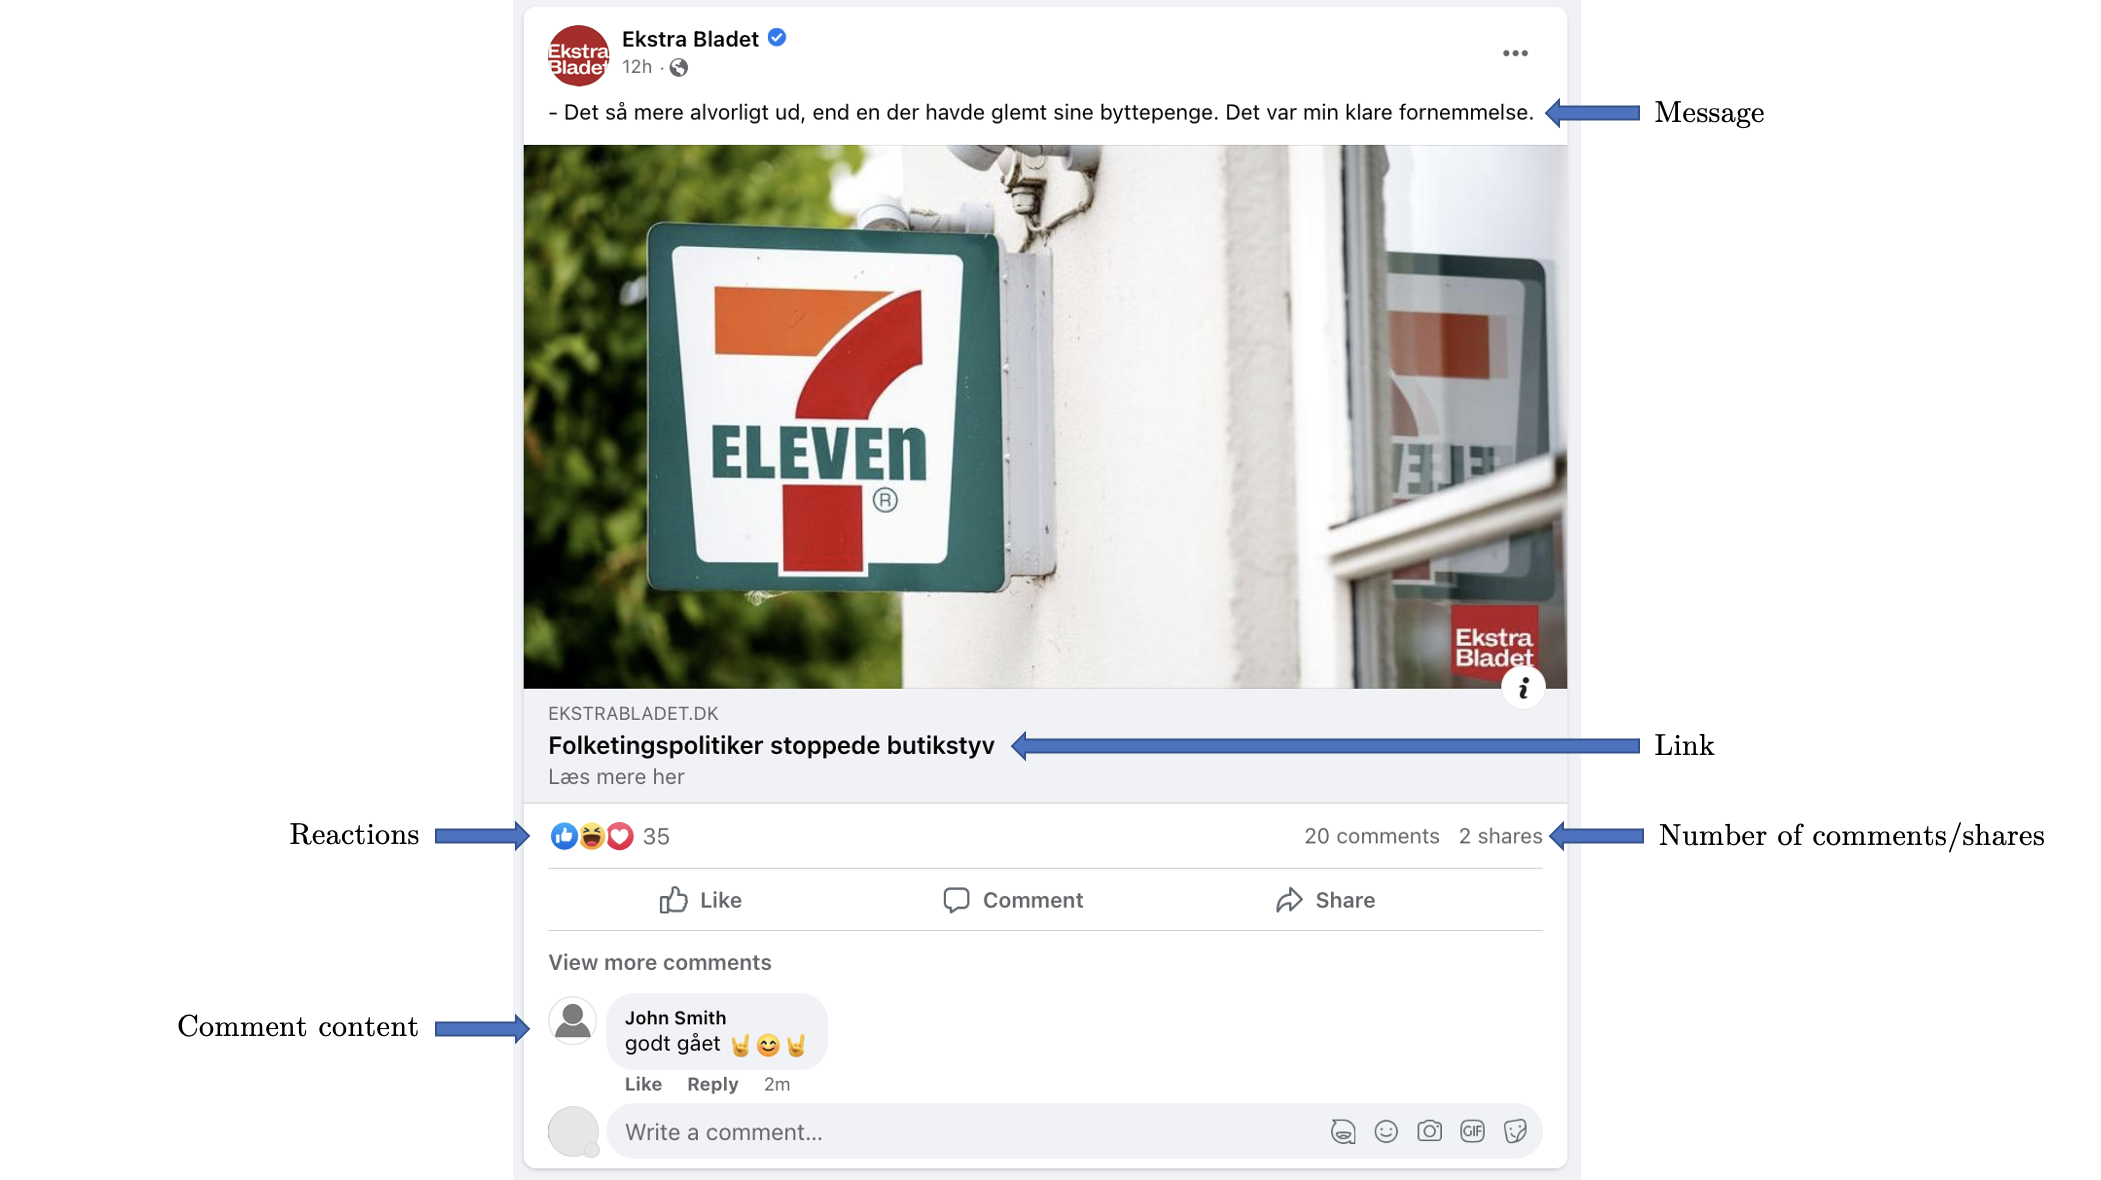
\includegraphics[width=0.8\linewidth]{images/facebook_post} 

}

\caption{Example of Facebook post}\label{fig:post_example}
\end{figure}

Even with our access to Facebook's API, it is not possible to extract
any kind of personal information such as usernames or user-IDs from the
comment section. While this limits some of the possible analysis, this
alleviates ethical concerns when dealing with digital trace data and
lessens the task of complying with the GDPR. However, in terms of data
validity, it is a limitation, since we do not know the number of unique
users commenting on a post, but only the content of the comments
themselves. This limitation is further discussed in Section 5.3.1.

Another concern of using Facebook's API is that we rely on their data
quality. During our process of validating the data quality, we found a
few cases where e.g., the number of reactions from the API did not match
the number of reactions shown on the post in the user interface. We
cannot for sure say what causes this inconsistency, as the API is not
well documented. However, the differences were often small and did not
look systematic, and such noise in data is common in studies of digital
trace data and social media (Salganik 2018:37).

\hypertarget{operationalization}{%
\subsection{Operationalization}\label{operationalization}}

The following sections describe our operationalizations -- how the
theoretical concepts are defined as empirical measurements. The first
section describes how the outcomes, the dimensions of audience
engagement on social media, are measured. The second section describes
how each of the predictors for news content are operationalized.
Finally, we present a range of control variables that we include to
adjust for possible confounding effects of our main predictors on the
outcomes.

\hypertarget{outcomes}{%
\subsubsection{Outcomes}\label{outcomes}}

\noindent In this study, the main concept of interest is audience
engagement on social media. As described in Section 3.1, we seek to
include a broad and multifaceted understanding of audience engagement.
Therefore, we define audience engagement as a number of different
behaviors that are theoretically rooted in different kinds of
motivations based on previous studies and theory. We have identified
four different dimensions of audience engagement: information selection,
emotional responses, sharing, and conversations. In the following, we
describe how these four dimensions are measured using eight different
outcomes.

The outcome variables are measured either as counts or proportions.
Generally, metrics based on the content and structure of the
comment-section are treated as proportions while the rest are counts.
While the proportions may produce outliers in case of posts with very
few comments, the advantage of using proportions rather than counts is
that it allows us to account for the overall volume of engagement, and
as such avoid post popularity to determine too much of the variance.

\hypertarget{information-selection-1}{%
\paragraph*{Information Selection}\label{information-selection-1}}
\addcontentsline{toc}{paragraph}{Information Selection}

\hspace{-2.5em}

\noindent One dimension of audience engagement is the behavior of
information selection. In other words, it is behavior where the audience
actively chooses to read, view, or expose oneself to the news content.
As described in Section 2.3.3., this behavior might be related to a
motivation of wanting to obtain information or knowledge about the news
content. As an empirical measurement of the dimension of information
selection, we use the number of times someone has clicked on the link on
the shared article. All posts on Ekstra Bladet's Facebook page contains
a link to an article on their website, ekstrabladet.dk. By using
meta-tags in the HTML-header on their webpage, Ekstra Bladet defines
which title and picture should be used when sharing a link to the page
on Facebook. In this way, the post is formatted with the correct title
and picture from the article (see Figure 1). To our knowledge, only one
other very recent study has used this kind of data in relation to social
media engagement (Robertson et al.~2023).

\hypertarget{emotional-responses-1}{%
\paragraph*{Emotional Responses}\label{emotional-responses-1}}
\addcontentsline{toc}{paragraph}{Emotional Responses}

\hspace{-2.5em}

\noindent Another dimension of audience engagement is tied to the
emotional responses to the news content. For this engagement, the
underlying motivation might be to interpret or decode the news content
and consequentially a specific emotion or opinion might appear. As
described in Section 2.3.4., emotional responses usually refer to felt
engagement rather than a behavioral engagement. However, Facebook has
enabled the manifestation of the felt engagement into behavioral
engagement by making it possible to react with an emoji to the content.
Therefore, this study uses the total number of reactions on each post as
an empirical measurement of emotional responses. From 2016, several
reactions representing different feelings were introduced in addition to
the traditional like (Meta 2016). Currently, it is possible to react on
Facebook with one of the reactions named: like, love, care, haha, wow,
sad, and angry. Figure 2 below shows the emojis representing the
possible reactions on Facebook. Unfortunately, the care-reaction is not
available in the API, from which we collect the data, and therefore we
cannot use it in our analysis.

\begin{figure}[H]

{\centering 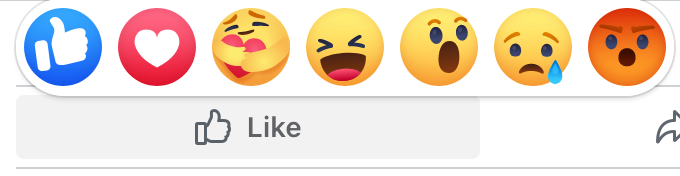
\includegraphics[width=300px]{images/reactions_example} 

}

\caption{Reactions on Facebook}\label{fig:reactions_example}
\end{figure}

\noindent Some studies have examined how different reactions signify and
represent different kind of emotional responses to the content, while
others combine the total count of reactions as a measure of general
valence or emotional arousal (León \& Trilling 2021; Heidenreich et
al.~2022). Although it could have been interesting to examine how
different kinds of emotional responses might differ in their relation to
news content, we chose to only include an aggregated count of all
reactions as a measure of general emotional valence.

\hypertarget{sharing}{%
\paragraph*{Sharing}\label{sharing}}
\addcontentsline{toc}{paragraph}{Sharing}

\hspace{-2.5em}

\noindent Yet another dimension of audience engagement is the behavior
of sharing new content. As described in Section 2.3.5., sharing might be
related to different kinds of motivations. If sharing is directed
towards one's entire social network, it might be related to gaining
social status, while sharing behavior directed at a specific person
might be related to phatic sharing that is a way of maintaining specific
social ties. To capture these two types of sharing, this study includes
two different measurements of sharing behavior: 1) the number of times a
post has been shared onto a user's feed, and 2) the proportion of
mention comments in the comment section.

Sharing a post on Facebook means that the post is shared on your own
profile, and it is likely to appear in your friends' feed. It is not
directed at specific people, but it will be shown to your entire network
of friends. In addition to this, we also introduce a second novel
measurement of the proportion of comments that can be understood as a
mention comment. When writing a comment to a post, it is possible to tag
other users, and they will get a notification that they have been
mentioned in a comment. Some comments do not contain any supplementary
text other than perhaps an emoji or two, and we argue that these
comments are a different type of comment than regular comments -- a
different method for engaging with content in a specific relational
manner. Figure 3 below shows an example of such ``mention.''

\begin{figure}[H]

{\centering 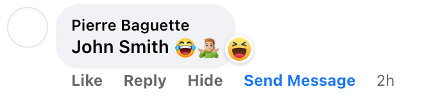
\includegraphics[width=0.8\linewidth]{images/mention_example} 

}

\caption{Example of a mention comment}\label{fig:mention_example}
\end{figure}

\noindent These mention comments represent sharing, but in a different
way than when sharing the post to your own feed. Mention comments are
directed towards a specific person as a way of telling the person that
this content is particularly relevant to the person. In this way, it is
reminiscent of the idea of phatic news sharing described by Duffy \&
Ling (2020), whereas sharing the post to your own timeline might to a
larger degree represent a sharing-behavior directed at self-expression,
social status, or informational sharing (See Section 2.3.5.).

\hypertarget{conversations-volume-reciprocity-and-respect}{%
\paragraph*{Conversations: Volume, Reciprocity, and
Respect}\label{conversations-volume-reciprocity-and-respect}}
\addcontentsline{toc}{paragraph}{Conversations: Volume, Reciprocity, and
Respect}

\hspace{-2.5em}

\noindent The final dimension of audience engagement included in this
study is the behavior of having conversations about news content. As
described in Section 2.3.6., there can be many different motivations
related to the behaviors of discussing news content. First of all, there
might be motivations that are related to the general behavior of
actually having a conversation rather than lurking or keeping opinions
to oneself. However, this motivation relates only to the volume of
conversations and not the content of the comments or the quality of
conversations that is required in the theories of deliberative
democracy. The presence of comments and conversations could signify a
motivation to express opinion, but it is different motivations that
relate to how deep or respectful the conversations are. Furthermore, the
behavior of having conversations might also be motivated by sincerity,
empathy, or respect to engage with each other, or it might be motivated
by disrespect, anger, or strategic motivations. Thus, the dimension of
audience engagement of having conversations is operationalized as four
different empirical outcomes in this study inspired by the study by Esau
et al.~(2017): the volume of conversations, the reciprocity of
conversations, and the disrespect and respect of the conversations.

The volume of conversations is measured empirically using the number of
comments on each post. The count of comments also includes reply
comments (when a comment is a reply to another comment or reply rather
than a comment on the post itself) and mention comments. This outcome is
the measure of the quantity of comments, while the remaining measure
different kinds of qualitative indicators. While the measurement of
volume is not a part of Esau et al.'s original dimensions, we argue that
it is an important prerequisite since it may indicate both that a
broader audience is engaged, and more diverse opinions are shared.

The reciprocity can be understood as the depth of the conversation,
e.g., to which degree the comments address other comments. To measure
reciprocity in this study, we use the proportion of reply-comments out
of all comments. Replies are different from ordinary comments, as they
are a response to another comment or reply, while comments can only be
responses directly to the post. In our analysis, we do not distinguish
between replies that are directed at other replies or replies that are
directed at comments. The share of replies is generally a representation
of how nested the conversation in the comment section is, i.e.~how much
dialogue takes place.

To measure disrespect and respect of conversations in this study, we use
the proportion of comments with offensive language and the proportion of
comments with recognizing language. In previous studies, respect has
only been understood as the absence of offensive or hateful language,
but other studies have argued that positive aspects of respect should
also be included such as comments that contain constructiveness,
empathy, or recognition (See Section 2.3.6.).

To create a measure of how many comments contain offensive or
recognizing language, we use two different models developed by Analyse
\& Tal (2021) to detect these linguistic traits. Multiple models for
detecting offensive language in Danish have been developed
(Sigurbergsson \& Derczynski 2019), while only one model for detecting
recognition in Danish exists. In Analyse \& Tal's work, recognition is
defined as a complex concept comprised of statements of empathy, praise,
or openness, targeted towards another human being (Analyse \& Tal
2021b). They draw on a broad range of literature, including Kierkegaard,
Hegel, and Honneth, highlighting relationships and respect as important
aspects (ibid:14b). As a part of their operationalization, they further
define eight forms of recognition: praise and agreement, empathy,
acknowledgment of other views and arguments, curiosity, openness,
expression of susceptibility or self-doubt, expression of desire for
dialogue, trust, and ritual recognition. On the other hand, offensive
language is defined as any stigmatizing, offending, stereotyping, or
threatening utterances (Analyse \& Tal 2021a).

Both models are based on a Danish pretrained version of the transformer
model architecture, Electra (Højmark-Bertelsen 2021; Clark et al.~2020).
Transformer models are state-of-the-art deep learning architecture for
dealing with text data (Wolf et al.~2020). The Electra model is
pre-trained on a large quantity of text, where the task is to predict
masked words in the text. By doing this, the model gains a numerical
representation of text in general, which can then be used for other
tasks, such as classification. A standard way of evaluating
classification models is by using F1-scores in which zero is the lowest
value and a score of 1 would be a perfect model. In our case the macro
average F1 score is used as a metric to evaluate the performance of a
multi-class classification model. It is calculated by first computing
the F1 score for each class separately and then taking the average of
all the F1 scores. In other words, macro average F1 score gives equal
weight to each class, regardless of its size or distribution. Both
models by Analyse \& Tal have a performance around 0.8 measured with a
macro average-F1-score (Analyse \& Tal 2021). Figure 4 and 5 below show
examples from our data of predictions of both comments with offensive
language and recognizing language.

\begin{figure}[H]

{\centering 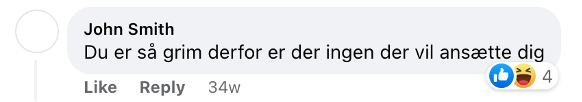
\includegraphics[width=300px]{images/offensive_language} 

}

\caption{Example of a comment with offensive language}\label{fig:offensive_example}
\end{figure}

\begin{center}
\small
\emph{"You are so ugly which is why no one wants to hire you"}
\end{center}
\normalsize

\begin{figure}[H]

{\centering 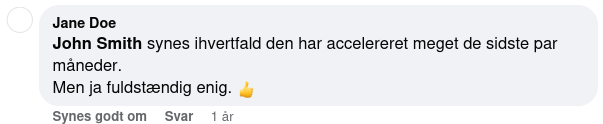
\includegraphics[width=300px]{images/recognizing_language} 

}

\caption{Example of a comment with recognizing language}\label{fig:recognition_example}
\end{figure}

\begin{center}
\small
\emph{"John Smith in any case, it seems to have accelerated a lot in the past few months. But yes, I totally agree."}
\end{center}
\normalsize

\noindent We have manually inspected samples of the predictions from the
models, and there are a few nuances to consider. For one thing, a
comment can contain both offensive language and recognition at the same
time. An explanation of this might be that a comment can contain both
anger towards one person and empathy towards another person in the same
argument. In addition to this, a limitation of these classification
models is that they do not take the context of social relations or the
other comments in the thread into consideration. We discuss this
limitation further in Section 5.3.1.

\hypertarget{subconclusion-outcomes}{%
\paragraph*{Subconclusion: Outcomes}\label{subconclusion-outcomes}}
\addcontentsline{toc}{paragraph}{Subconclusion: Outcomes}

\hspace{-2.5em}

\noindent In this section, we described how our multifaceted
understanding of audience engagement has been operationalized into
empirical measurements. Table 1 below presents an overview of the four
dimensions of audience engagement and their eight empirical
measurements. The second column describes the possible motivations that
we have considered based on previous theory and research. While
extensive, this operationalization should not be seen as a coherent
theory, since developing a unified framework for understanding behavior
and motivations lies beyond the scope of this study. Instead, they
represent possible mechanisms which we will discuss in relation to our
empirical results. In the next section, we present the empirical
measurements of the predictor variables as different measurements of
news content.

\begin{table}[H]
\caption{\label{operationalization-table}Outcomes}
\centering
\resizebox{0.85\textwidth}{!}{%
\begin{tabular}{@{}lll@{}}
\toprule
\textbf{Dimension of Audience Engagement} & \textbf{Possible motivations}                           & \textbf{Empirical Outcome}              \\ \toprule
Information   Selection          & Knowledge   gaining or entertainment           & Number   of link clicks        \\ \midrule
Emotional   Responses            & Interpretation   or opinion-making            & Number   of reactions          \\ \midrule
\multirow{2}{*}{Sharing} & Social   status              & Number   of shares                   \\
                         & Maintenance   of social ties & Proportion   of mention comments     \\ \midrule
\multirow{4}{*}{Conversations}   & Expression   of opinion                       & Number   of comments           \\
                                 & Reciprocity or dialogue & Proportion   of reply comments \\
                         & Disrespect                   & Proportion   of offensive comments   \\
                         & Respect or empathy           & Proportion   of recognizing comments \\ \bottomrule
\end{tabular}%
}
\end{table}

\hypertarget{predictors}{%
\subsubsection{Predictors}\label{predictors}}

\noindent The predictors in the analysis are the news content
characteristics from news value theory and related concepts such as
spreadability and the distinction between hard and soft news (see
Section 2.4.). In most previous studies these news content
characteristics have been manually labelled, but in this study, we take
a different approach, which allows us to create a much more
comprehensive dataset (See Section 3.1). In the following section, we
describe how each news content characteristic is operationalized in our
analysis.

\hypertarget{timeliness-and-unexpectedness}{%
\paragraph*{Timeliness and
Unexpectedness}\label{timeliness-and-unexpectedness}}
\addcontentsline{toc}{paragraph}{Timeliness and Unexpectedness}

\hspace{-2.5em}

\noindent The news content characteristic of timeliness refers to the
article containing something that is new, recent, or ongoing. In the
articles by Ekstra Bladet, it is common to refer to stories that are
ongoing by writing \emph{``LIVE''} in the headline or
\emph{``Opdateres''} (Eng: is updated) in the subtitle or accompanying
message on Facebook.

To construct this measurement, we use regex (regular expressions - a way
of creating structured pattern matching for text content based on a
sequence of characters) to check whether the title, subtitle, or message
(the added description in the Facebook post) contains any of these
words. In the regex-matching, the casing of the letters is ignored. We
do not check the body of the article, as it would return too many false
positives, where the word could be used in different contexts.
Furthermore, the title and subtitle represent a resume of the content,
and it is often also where the framing and relevance of the article is
most clear (Dor 2003).

For the news content characteristic of unexpectedness, we use a similar
approach. Here, we define a regex to check the title, subtitle, or
message for any of the words \emph{``chok''} (Eng: shock),
\emph{``overraskelse''} (Eng: surprise), \emph{``afsløring''} (Eng:
revelation), \emph{``sensation''}, \emph{``usædvanlig''} (Eng: unusual).

\hypertarget{geographical-and-cultural-proximity}{%
\paragraph*{Geographical and Cultural
Proximity}\label{geographical-and-cultural-proximity}}
\addcontentsline{toc}{paragraph}{Geographical and Cultural Proximity}

\hspace{-2.5em}

\noindent Geographical and cultural proximity means that the news
content is relevant or near the audience by using either geographical or
cultural references. In order to measure whether the article content
contains such references, we draw on techniques from natural language
processing and use a machine learning model trained on the task of named
entity recognition (NER). NER is a technique to classify whether each
word in a text represents a predefined label such as persons,
geographical locations, or organizations. Figure 6 below shows two
examples of article titles and subtitles with NER predictions.

\begin{figure}[H]

{\centering 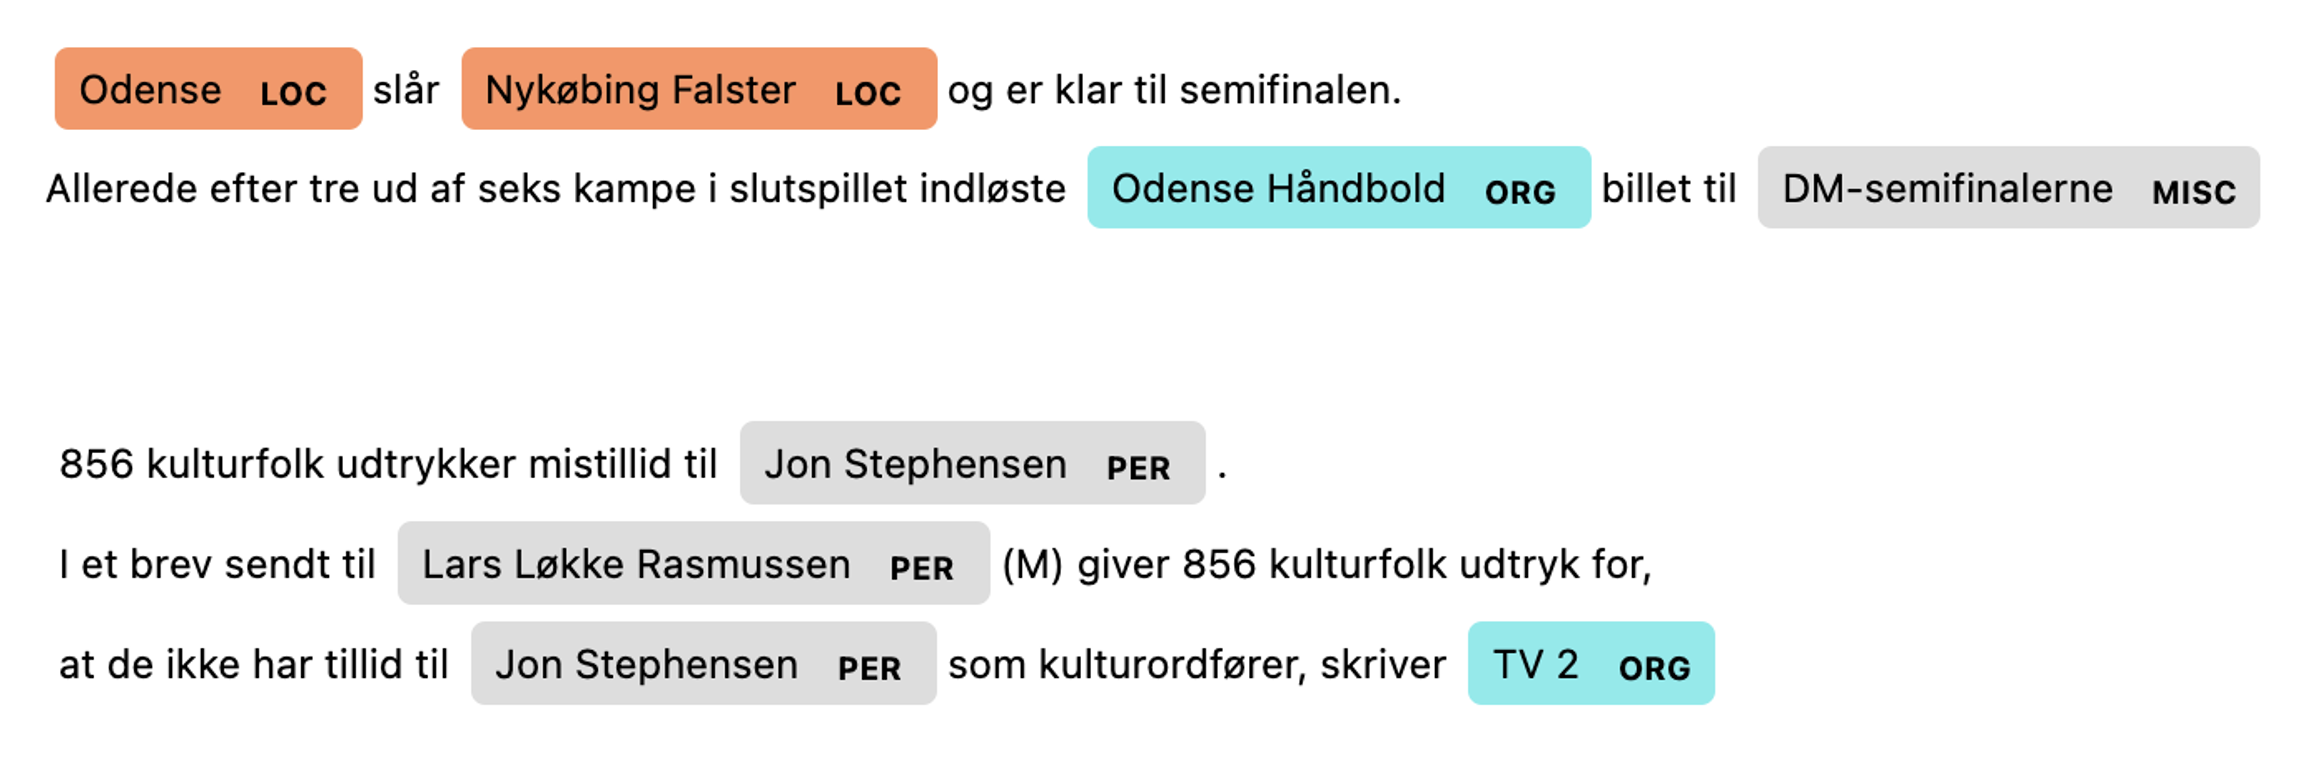
\includegraphics[width=400px]{images/ner_examples} 

}

\caption{Examples of NER classification of title and subtitles}\label{fig:ner_example}
\end{figure}

\begin{center}
{\footnotesize \emph{The label PER is persons, LOC is locations, ORG is organizations, and MISC is miscellaneous.}}
\end{center}

\noindent The specific model we use is a transformer-based model trained
by Ekstra Bladet, which achieves an F1-score of 0.93 on a test-dataset
of articles from Ekstra Bladet. As geographical proximity, we match the
predicted geographical locations with a list of Danish geographical
entities extracted from Danmarks Adressers Web API (DAWA). Thus, we
argue that an article contains content that is geographically near if it
contains a Danish geographical location. For cultural proximity, we
argue that references to organizations could be used as a novel
measurement. Cultural references vary from individuals, and therefore it
might be difficult to determine the general cultural proximity of a news
story based on the entire possible population of readers. However, when
articles reference a specific named organization in the headlines, it
could be the name of a sports club, a company, or an interest
organization, and to do so might invoke a sense of a shared cultural
frame.

The separation of cultural and geographical proximity into two different
measurements is supported by our talks with Ekstra Bladet's social media
team (see Section 3.5.3. for further elaboration). As an example, one of
the social media editors from Ekstra Bladet explained how they would
highlight news stories differently: when referring to a news story about
an incident in a church in a Danish town, Ribe, they argued the
significance of mentioning Ribe to capture geographical proximity. On
the other hand, if something happened in a McDonalds in an American
city, the fact that it happened in a McDonalds would be emphasized,
since this is the cultural reference to which people can relate to. In
this case, the Danish town Ribe would match a Danish geographical
location, while McDonalds would match the entity of an organization and
thus cultural proximity.

\hypertarget{personalization}{%
\paragraph*{Personalization}\label{personalization}}
\addcontentsline{toc}{paragraph}{Personalization}

\hspace{-2.5em}

\noindent The referencing of persons in news content refers to both the
news values of eliteness and non-eliteness. On the one hand, referencing
people that are famous or have high social status might drive relevance
in some contexts, and on the other hand referencing non-elite actors,
who the audience can relate to, might also drive relevance in other
contexts. To measure the references of persons in the article content,
we also use the technique of NER. Examining the frequency counts of the
extracted matches, we see that they can mostly be interpreted as elite
people. Even the persons that only appear once in an article headline or
subtitle are often famous to the general Danish public. Therefore, we
argue that this measure is primarily an operationalization of
personalization (elite). We have tested alternative ways to measure
referencing of non-elite person in the text, but the quality was
unsatisfying. As a consequence, we do not use the news value of
non-elite personalization in this analysis, which is a limitation to the
study. Instead, we only include eliteness, which we will just call
personalization in the remaining sections.

\hypertarget{negativity-and-positivity}{%
\paragraph*{Negativity and Positivity}\label{negativity-and-positivity}}
\addcontentsline{toc}{paragraph}{Negativity and Positivity}

\hspace{-2.5em}

\noindent The news content characteristics of negativity and positivity
can be tricky to operationalize. In previous research, different
concepts such as sentiment, emotionality or valence are used. Whether
content is positive, negative, or neutral can be understood as both
explicit and implicit (Van de Kauter et al.~2015). By explicit, the
content itself contains language that can be interpreted as negative or
positive. On the other hand, implicit implies that the wording itself
can be neutral, but that the content or topic refers to something that
is negative or positive. Therefore, we argue that negativity and
positivity can both be based on the topic or the style of the news
content. For negativity, we are able to construct measures based on both
the topic and style, while we are only able to construct measures based
on the style for positivity.

The measurement of negativity based on the topic is made using a machine
learning model predicting the topics of the article. This model is a
transformer-model trained by Ekstra Bladet, and it predicts the highest
probable topics of the article out of a list of 21 predefined topics. On
a test-dataset of articles, the model achieves an F1-score of 0.81. We
define that the news content contains negativity based on the topic when
the model predicts any of the topics: catastrophe, conflict and war, or
crime. These topics are inherently negative, while we were not able to
define any topics as exclusively positive.

To construct a measurement of negativity and positivity based on the
style, we evaluate multiple different approaches. Sentiment
classification is a large area of research within the field of natural
language processing, although it has mostly been applied to texts with
explicit expressions such as product reviews or social media, but to a
less extent news content (Hamborg \& Donnay 2021). As a consequence, no
available sentiment classification models pretrained on the domain of
news content in Danish, and we therefore choose to use a model
pretrained on a different domain. To evaluate which approach would be
optimal for this specific task, we labelled a sample of 500 articles
from our dataset to use as a test dataset. Previous annotation-schemes
for sentiment have been defined as attitudes towards a specific target.
We argue that this is less relevant in the domain of news content, and
that a more suitable definition is to consider sentiment as the imagined
attitude of the author of the text (Hamborg \& Donnay 2021:1666). We use
this definition for annotating the test dataset. We use only the text
from the title and subtitle of the article, as this headline is
understood to contain the discursive framing of the article (Dor 2003).
First, both authors labelled 100 articles, with an achieved
inter-coder-reliability of 70\%. We then discussed the diverging cases,
and subsequently labelled the 400 remaining articles. The relatively low
inter-code-reliability could possibly have been improved if the coders
had undergone a more extensive training process, but since producing a
high-quality benchmark dataset is not the scope of this study, we found
the reliability acceptable.

On this test set, we evaluated five different models: AFINN which is a
lexical approach to sentiment analysis (Nielsen 2011), SENDA (Platform
Intelligence in News 2022) and BERT Tone (Alexandra Instituttet 2023)
which are transformer-based sentiment classification models, ScandiNLI
which is a natural language inference model (Nielsen 2023), and finally
GPT-3.5-turbo (OpenAI 2023) which is a transformer-based large language
model (LLM) that we prompt-engineered for the sentiment classification
task. These models represent different approaches to sentiment
classification, and therefore we can evaluate which approach is most
useful for our specific task and domain. Section 8.2. in the Appendix
shows the performance of each model on our test set. ScandiNLI has the
highest F1-score (0.70) -- just a slightly better performance than
GPT-3.5-turbo -- and therefore we use this model to predict on our full
dataset for analysis. Although the best performing model does not yield
an astonishing performance, it is at the same level as the manual
labelling of sentiment, and we therefore find it acceptable for the
present study.

\hypertarget{impact}{%
\paragraph*{Impact}\label{impact}}
\addcontentsline{toc}{paragraph}{Impact}

\hspace{-2.5em}

\noindent The news content characteristic of impact refers to content
that has significant consequences or extraordinary relevance. In this
study, we argue that the concept of breaking news is a good measurement
of when content is of significant impact. The concept of breaking news
can be traced back to Associated Press in 1906, who coined the concept
as \emph{``news of transcendent importance''} (Pennington 2021:214). In
the same way, we argue that content labelled as breaking still
represents the most impactful or significant news stories. In our
dataset, it is defined by the editors and journalists of Ekstra Bladet
when an article is considered breaking, and we get that information from
Ekstra Bladet's database. There are no formal guidelines or rules for
when news content should be labelled as breaking news, which falls in
line with the classical idea of breaking news as something that
\emph{``you know when you see it''} (Pennington 2021:214). If an article
is labelled as breaking news, the article is automatically presented
with a yellow background on the website, and users of their app will get
a push-notification. However, there are not any automatic differences on
the shared article on Facebook, but here the framing is made by the
social media editors, who often write ``BREAKING'' in the accompanying
message of the shared link.

A limitation of using breaking news as a measure of impact is that some
also interpret breaking news as related to the news value of timeliness.
The idea of breaking news is not only that it is of significant societal
impact, but also that it has just happened (Pennington 2021:214).
However, we argue that in our case most of the news content on Ekstra
Bladet has relatively just happened, and that the importance is on what
they emphasize when presenting the news content.

\hypertarget{spreadability}{%
\paragraph*{Spreadability}\label{spreadability}}
\addcontentsline{toc}{paragraph}{Spreadability}

\hspace{-2.5em}

\noindent The news content characteristic, spreadability is specifically
used for news content on social media. Spreadability refers to news
content that is optimized for sharing, commenting and remixing in
various ways (Jenkins et al.~2013; Harcup \& O'Neill 2017). News content
with spreadability is content that directly prompts the audience to
interact with each other instead of just seeking individual attention
(Jenkins et al.~2013:4). To measure spreadability, we check whether the
message of the post contains a question mark at the end. Asking a
message in the question have previously been shown to drive to greater
user engagement (Quesnelle \& Montemayor 2020). Furthermore, we argue
that the question framing represents a prompt aimed directly at the
audience to make them engage and interact with the post.

\hypertarget{hard-news}{%
\paragraph*{Hard News}\label{hard-news}}
\addcontentsline{toc}{paragraph}{Hard News}

\hspace{-2.5em}

\noindent The final news content characteristic included in our study is
the difference between hard and soft news. In news value theory, this is
often mentioned as the news value of entertainment. As described in
Section 2.4.3., hard and soft news is an often used, but also
ambiguously defined concept in both media studies and media
organizations. In this study, we define hard and soft news in terms of
the topic of the news content rather than style or framing (Reinemann et
al.~2012:234).

When hard or soft news is defined by topics, it refers to whether the
news content address heavier topics of societal relevance such as
politics, economy, or science on the one hand or topics related to
entertainment such as lifestyle, celebrities or similar on the other. To
measure hard news topic in this study, we use the machine learning model
trained by Ekstra Bladet to predict topics of the article that we also
use for measuring negativity based on the topic. Out of the list of 21
pre-defined topics, we argue that hard news topics are: business,
politics, society, health, science, and economy, while the remaining
topics are more likely to be soft news topics.

\hypertarget{subconclusion-predictors}{%
\paragraph*{Subconclusion: Predictors}\label{subconclusion-predictors}}
\addcontentsline{toc}{paragraph}{Subconclusion: Predictors}

\hspace{-2.5em}

\noindent In this section, we described how the news content
characteristics are operationalized into empirical measurements. In
contrast to previous studies, we do not rely on manual labelling of the
news content but use methods from the field of natural language
processing to label the news content. The strength of this approach is
that it can be used on huge datasets that would not be feasible to label
by hand. Table 2 below summarizes the concrete operationalizations of
each news content characteristic that we use as predictors in our
analysis. All measurements are dummies.

\begin{table}[H]

\caption{\label{tab:predictors_opera}Predictors}
\centering
\begin{tabular}[t]{l>{\raggedright\arraybackslash}p{8cm}}
\toprule
News content characteristic & Empirical measurement\\
\midrule
Timeliness & Contains any of “LIVE”, “opdater” in the message.\\
Unexpectedness & Contains any of “chok”, “overraskelse”, “afsløring”, “sensation”, “usædvanlig”,”mirakuløs”,  “opsigt”, ”vild” in title.\\
Geographical Proximity & Contains a location (LOC) NER-tag matched with a list of Danish locations in either title or subtitle.\\
Cultural Proximity & Contains an organization (ORG) NER-tag in either title or subtitle.\\
Personalization (elite) & Contains a person (PER) NER-tag in either title or subtitle.\\
Negativity (topic) & Has predicted topic of either “konflikt og krig”, “katastrofer”, “kriminalitet”.\\
Negativity (style) & Has predicted “negative” sentiment (ref. neutral)\\
Positivity (style) & Has predicted “positive” sentiment (ref. neutral)\\
Impact & Is “breaking news”\\
Spreadability & Message contains “?”\\
Hard news & Has predicted topic of either “erhverv”, “politik”, “samfund”, “sundhed”, “videnskab”, ”økonomi” (ref. soft)\\
\bottomrule
\end{tabular}
\end{table}

\hypertarget{control-variables}{%
\subsubsection{Control variables}\label{control-variables}}

\noindent In our analysis, we include a few additional measurements that
are important to control for. First of all, we control for the fact that
the article may be behind a paywall. This restrictiveness to the full
content of the article could influence the different levels of
engagement. Furthermore, we include two control variables related to
different time periods. We control for the time of day, i.e., posts
posted PM or AM. We also control for the day of the week, by including a
binary variable for weekends or weekdays. We include these control
variables, since both engagement and the selection of news articles may
vary for both time of day and day of week, which is supported by our
talks with the moderators (see Section 3.5.3.).

Another possible source of bias is the internal rules and strategies for
selecting of what content to post among the social media editors at
Ekstra Bladet. For example, the social media team at Ekstra Bladet
changed their social media strategy from the 1\textsuperscript{st} of
May 2022 deciding to reduce the frequency of sharing posts on their
Facebook page. This can be seen quite drastically in Figure 7 below
showing the number of articles posted on their Facebook page per week
during the period.

\begin{figure}[H]

{\centering 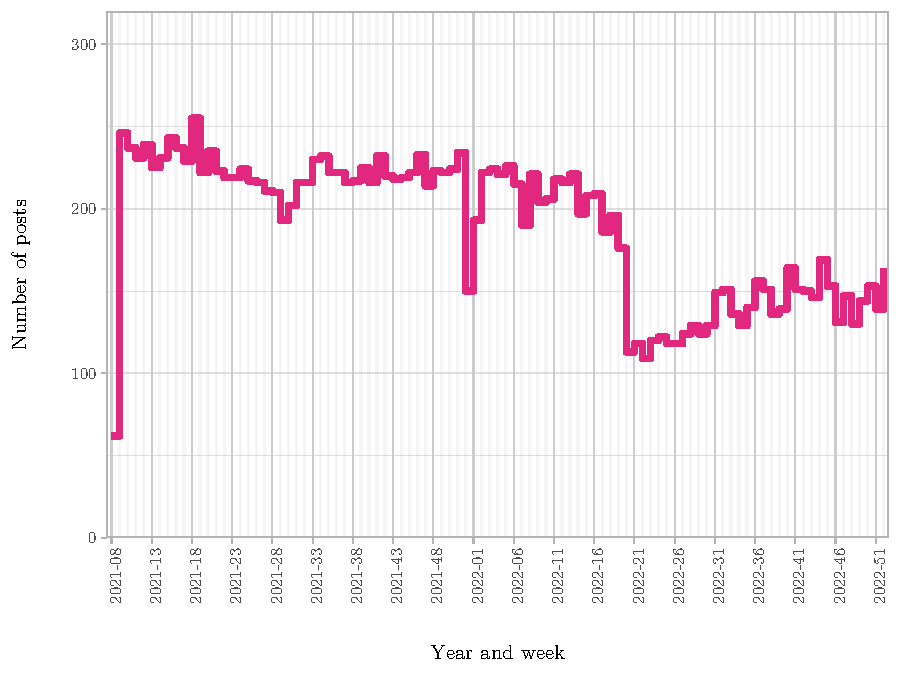
\includegraphics[width=400px,height=200px]{paper_files/figure-latex/posts_per_week-1} 

}

\caption{Number of Facebook posts per week}\label{fig:posts_per_week}
\end{figure}

\noindent Third parties such as researchers are commonly unaware of such
internal, strategic decisions, but nonetheless these decisions might
have a significant impact on the dynamics of the audience engagement.
This is another example of how our collaboration with Ekstra Bladet has
yielded an important background knowledge of our case of study. In order
to control for this change in social media strategy, we include a
control variable capturing whether the article is posted during the
previous or current internal strategy.

In addition to the confounding bias by internal decisions by the media
organization, there might also be macro-level influences that affect the
influence of news content on audience engagement. For example, the act
of holding an election is a significant societal event that has the
potential to change the relation between news content and audience
engagement. During an election, audiences might engage more intensely
with political or societal issues than during other periods (Strömback
\& Johansson 2007). In the period included in our data, there was a
national election, and this event could affect the audience to be more
interested in news content about politics than in average during the
entire period. Therefore, we include a control variable for whether the
article is posted during an election period or not. Table 3 below
summarizes the control variables included in our analysis.

\begin{table}[H]

\caption{\label{tab:controls_opera}Control variables}
\centering
\begin{tabular}[t]{l>{\raggedright\arraybackslash}p{8cm}}
\toprule
Control Variables & Operationalization\\
\midrule
Pay-wall & From Ekstra Bladet’s database\\
Time of day & Is posted from 12.00-00.00 (PM) (ref. posted from 00.00-12.00 (AM))\\
Day of week & Is posted in the weekend (SAT, SUN) (ref. posted on a weekday (MON,TUE,WED,THU,FRI)\\
Strategy Change & Article has been posted after strategy change (from 1st of May or later) (ref. before)\\
Election Period & Article has been posted during a national election period (5th of October 2022 to 1st of November 2022) (ref. outside)\\
\bottomrule
\end{tabular}
\end{table}

\hypertarget{methods}{%
\subsection{Methods}\label{methods}}

In this section, we describe the methods that we use to analyze how news
content influences audience engagement. In the first part, we consider
different distributions and our choice of regression design as proof of
association. In the second part, we describe our methodological approach
of evaluating validity through theory-based data analysis.

\hypertarget{regression-design}{%
\subsubsection{Regression Design}\label{regression-design}}

\noindent In order to analyze the influence of news content on audience
engagement, we employ eight different regressions -- one for each
outcome of audience engagement. For all eight regressions, we use a
multiple linear regression estimated with ordinary least squares (OLS).
To accommodate for heteroscedasticity, we calculate robust standard
errors. Multiple linear regression with OLS is perhaps the most common
regression model, and while it serves as a versatile tool, there are
also a couple of limitations of this regression design. For example,
linear regression assumes that a unit increase of the predictor leads to
a constant change for the outcome. Thus, it is also assumed that the
distribution of the outcomes can be any value from
\(-\infty \rightarrow \infty\). However, that is not the case for any of
our outcomes in the analysis. Instead, four of our outcomes are counts,
i.e., they can range from \(0 \rightarrow \infty\), but only integer
values, and the remaining four outcomes are proportions, i.e., they can
range any value from \(0 \rightarrow 1\). For example, it is not
possible to have a negative number of comments or more than 100\%
offensive comments on a post. In principle, it might be more suitable to
use other kinds of regression models such as Poisson-regression for the
count-distributed outcomes, and a Beta-regression for the
proportion-distributed data.

Considering the distribution of our outcomes, it is also apparent that
all the measurements of audience engagement are far from normally
distributed, and often highly skewed towards zero. The distributions of
the outcomes tend to be power-law-distribution with a small minority of
observations having extremely high values compared to the majority of
observations. A limitation of linear regression is that it can be prone
to outlier observations that might be too influential on the coefficient
estimates (Van der Meer et al.~2010). However, we argue that these
outlier observations do not represent data errors, but rather extreme
values as part of the distribution, and therefore we should not exclude
them from our analysis.

As a consequence of these limitations, the linear model with OLS might
not be able to provide the best possible fit for our data. In our
analysis, this can be seen in the R\textsubscript{2}-values that are
quite low. Assessing alternative regression models to potentially
achieve a more optimal fit for our outcome distributions would have been
valuable. Nonetheless, such an exploration is beyond the scope of the
present study. Furthermore, we argue that the linear regression also has
an advantage in terms of explainability, as we are able to express the
coefficient estimates in absolute values rather than relative values.

As described, our dataset contains all articles shared during the period
of analysis, and therefore the analysis is based on the complete
population. Usually, this would imply that there is no need to infer
from a sample to a population, and statistical significance would be
irrelevant. However, we are still interested in generalizing from the
population to a superpopulation, i.e., articles shared on Facebook
before and after our period of study (see Section 5.4.). Therefore, the
analysis will still use measures of statistical significance to evaluate
the associations.

\hypertarget{theory-based-data-analysis}{%
\subsubsection{Theory-based Data
Analysis}\label{theory-based-data-analysis}}

\noindent While the empirical research design of this study is
correlational, the objective of the study is explanatory -- meaning that
we want to examine whether news content characteristics can causally
explain the audience engagement of the shared articles. However, the
causal mechanism cannot be fully confirmed based on our empirical setup,
and the causal validity of our results should be evaluated based on
synergy between theory and empirical results (Aneshensel 2013:20-21;
Agresti \& Finlay 1997).

Drawing on the approach of theory-based data analysis by Aneshensel
(2013), we understand our empirical results as the correlation of
measured variables that we use to make probable the underlying
mechanisms of the theoretical constructs (Aneshensel 2013:5). Studies
using big data and new methods from the field computational social
science have been criticized for being too inductive, too correlational,
and having a vague theoretical foundation (Cowls \& Schroeder 2015). To
address these concerns, our study prioritizes a solid and comprehensive
theoretical foundation to base our empirical results on more than just
correlational estimates. Following Agresti and Finlay (1997), empirical
association is only the first of three conditions that must be fulfilled
in order to claim a causal relationship. To validate a causal effect,
one must also consider a correct theoretical temporal sequence of the
phenomena and the elimination of alternative explanations of the
association (Agresti \& Finlay 1997:302-303). In Section 5.2., we
discuss our empirical results in relation to the theoretical temporal
sequence, and in Section 5.3. we consider any alternative explanations
of the findings.

\hypertarget{background-1}{%
\subsection{Background}\label{background-1}}

In this section, we examine the background of the case and empirical
analysis. While not directly related to our research question, we argue
that this descriptive information about the media and audience context
is important for the validity of our main analytical findings. First, we
consider the demographic distribution of Ekstra Bladet's audience on
Facebook. Secondly, we examine a potential selection bias by comparing
the characteristics of the articles shared on Facebook with all articles
published by Ekstra Bladet. Thirdly, we describe Ekstra Bladet's
strategies for engaging with their audiences on Facebook, and finally,
we consider how much of the Facebook engagement with Ekstra Bladet's
content we capture through their own Facebook page.

\hypertarget{ekstra-bladets-audience-on-facebook}{%
\subsubsection{Ekstra Bladet's Audience on
Facebook}\label{ekstra-bladets-audience-on-facebook}}

\noindent Our specific case of study is the relation between the Danish
media, Ekstra Bladet and their audiences on Facebook. In order to
interpret the analytical findings and possibly generalize or transfer
the findings to other cases, it is important to characterize the
specific audience of Ekstra Bladet.

The Facebook page of Ekstra Bladet has a little over 400,000 followers
(as per the 1\textsuperscript{st} of April 2023). 48\% of the followers
are men, while 52\% are women. Figure 8 below shows the distribution of
age and gender for both followers of the Facebook page and followers
actively engaging with content on the page from a sample of four weeks
from 1\textsuperscript{st}-28\textsuperscript{th} of February. As we
only have access to this aggregated demographic data, and since
Facebook's API documentation is inadequate, it is unknown to us how
Facebook specifically defines active engagement in this context.
However, it is likely that their definition overlaps with the
measurements included in our definition of audience engagement.

\begin{figure}[H]

{\centering 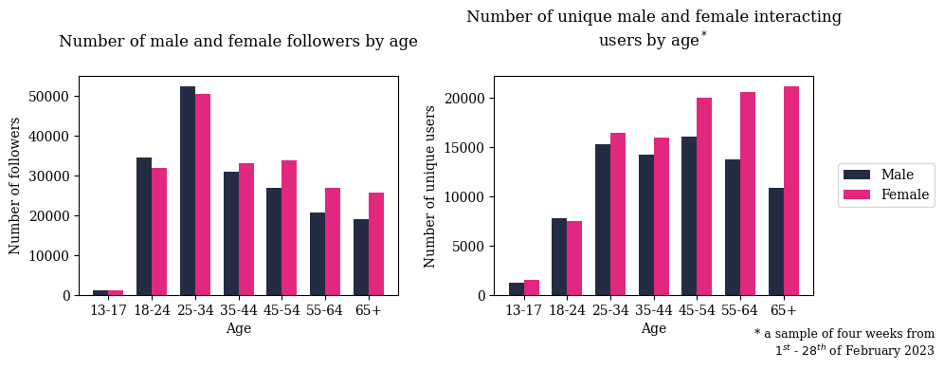
\includegraphics[width=0.8\linewidth]{images/fb_audience} 

}

\caption{Ekstra Bladet's Facebook audience demographics}\label{fig:fb_audience}
\end{figure}

\noindent As Figure 8 shows, Ekstra Bladet has very few followers, who
are younger than 18 years old, while the most frequent age group is
audiences between 25-34 years old consisting of about 25\% of all
followers. Fewer and fewer followers are found among older age groups,
especially for men. There are noticeable different demographic
characteristics when considering audiences, who just follow the page and
audiences, who actively engage with the content. When it comes to
audience, who actively engage with the news content, 43\% were males,
and 57\% were females. Especially for the ages 45 to 65+, there is a
large overrepresentation of women compared to men. An explanation of the
demographic difference between audiences, who follow Ekstra Bladet, and
audiences, who actively engage with the news content, might be that
Ekstra Bladet's content might cater more to this specific part of the
audiences. However, it might also be a result of different social media
usage patterns. For example, younger audiences are increasingly present
on different social media than Facebook - especially new social media
such as TikTok and Snapchat are increasingly popular -- while older
audiences still primarily use Facebook as their main platform (DR
Medieforskning 2022:14; Slots- og Kulturstyrelsen 2020:26). Furthermore,
studies on Facebook behavior have been shown that women generally tend
to be more active than men (McAndrew \& Jeong 2012).

\hypertarget{the-sample-of-articles-posted-on-facebook}{%
\subsubsection{The Sample of Articles posted on
Facebook}\label{the-sample-of-articles-posted-on-facebook}}

\noindent In the period of study, Ekstra Bladet published 80,285
articles on their website, but our dataset only contains the 18,350
articles that have also been shared on Facebook. Thus, out of all
articles published on the website of Ekstra Bladet, approx. 20\% are
shared on their Facebook page. As the responsibility for selecting
articles to share on Facebook is held by the social media editors, it is
possible that there are certain kinds of articles that are more likely
to be shared on Facebook, which might represent a potential selection
bias. However, it is important to note that the articles shared on
Facebook are our population of interest, as the study examines audience
engagement on social media specifically. In Table 4 below, we present
summary statistics of the presence of news content characteristics that
we use as predictors in the analysis while comparing the full sample
with the articles posted on Facebook.

\begin{table}[H]

\caption{\label{tab:bortfaldstabel}Descriptive statistics for all articles and only articles shared on Facebook}
\centering
\begin{tabular}[t]{l>{\raggedright\arraybackslash}p{3cm}>{\raggedright\arraybackslash}p{3cm}l}
\toprule
Variable & Article published on website & Articles shared on Facebook & X2-test\\
\midrule
Timeliness &  &  & X2=60.168***\\
... 0 & 91\% & 89\% & \\
... 1 & 9\% & 11\% & \\
Unexpectedness &  &  & X2=104.722***\\
... 0 & 95\% & 94\% & \\
... 1 & 5\% & 6\% & \\
Geographical proximity &  &  & X2=28.691***\\
... 0 & 88\% & 87\% & \\
... 1 & 12\% & 13\% & \\
Cultural proximity &  &  & X2=6.118**\\
... 0 & 99\% & 99\% \vphantom{1} & \\
... 1 & 1\% & 1\% \vphantom{1} & \\
Personalization &  &  & X2=0.19\\
... 0 & 99\% & 99\% & \\
... 1 & 1\% & 1\% & \\
Hard News &  &  & X2=786.276***\\
... 0 & 58\% & 47\% & \\
... 1 & 42\% & 53\% & \\
Negativity (topic) &  &  & X2=54.648***\\
... 0 & 75\% & 72\% & \\
... 1 & 25\% & 28\% & \\
Negativity (style) &  &  & X2=212.298***\\
... 0 & 78\% & 73\% & \\
... 1 & 22\% & 27\% & \\
Positivity (style) &  &  & X2=61.917***\\
... 0 & 91\% & 93\% & \\
... 1 & 9\% & 7\% & \\
Impact &  &  & X2=1402.972***\\
... 0 & 97\% & 90\% & \\
... 1 & 3\% & 10\% & \\
\bottomrule
\multicolumn{4}{l}{\rule{0pt}{1em}Statistical significance markers: * p<0.1; ** p<0.05; *** p<0.01}\\
\end{tabular}
\end{table}

\noindent As seen in Table 4, most of the news content characteristics
have a larger proportion among the articles shared on Facebook. For
example, 9.9\% of articles shared on Facebook contain the news value of
impact - defined as news articles that are breaking news - compared to
only 3.4\% among all articles published. For the distinction between
hard and soft news, 53.2\% of articles shared on Facebook are around
hard news topics such as politics, economy, health and more, while for
all articles from Ekstra Bladet only 41.7\% of articles are hard news
topics.

From Table 4, it is also apparent that some of the news content
characteristics are quite sparse. For example, it is less than 1\% of
the news content than contains cultural proximity or personalization.
Thus, there are only around 110 out of 18350 articles in our dataset
that contains cultural proximity.

For most of the news content characteristics except positivity,
personalization, and cultural proximity, we see that the articles shared
on Facebook contains more of every article trait. While there is a
selection process in the journalistic production phase before articles
are published, these differences show that there is also a selection
process when considering which articles to share on Facebook. Only the
most relevant stories become news articles, and only the most relevant
news articles are shared on their Facebook page. Furthermore, it seems
that the selection criteria are likely to also be based on the news
content features that we include in this study.

\hypertarget{social-media-strategy}{%
\subsubsection{Social Media Strategy}\label{social-media-strategy}}

\noindent As part of the collaboration of the study, we have had access
to talk with the people at Ekstra Bladet, who are responsible for
posting and moderating content of their Facebook page. The strategies
and norms for administering their Facebook page are also relevant to our
empirical study as they influence the selection and framing of news
content.

Based on our conversation with Ekstra Bladet, the strategy for what
articles is posted on Facebook is mostly based on the intuition of the
responsible social media editor. According to the editor, the intuition
or feeling for what content will be engaged with, is has been developed
through experience of posting content for a long time, and they only
sporadically use different analytics platforms to gain an understanding
of what performs well. Furthermore, there is no written or formal
strategy for posting content.

The social media editors describe that they think a lot about what kind
of content to post at specific times. According to them, certain content
is more favorably received during morning or evening hours, whereas
other content is more suitable to post on the weekend rather than a
weekday. In terms of determining criteria for selecting articles to
share on Facebook, the editors often mention traits that are reminiscent
of news value theory such as geographical, cultural proximity, or hard
news. They also describe that they often consider when to share articles
that are hidden behind a paywall -- those that can only be read with a
subscription. The descriptions of the social media strategy provided by
the social media editors at Ekstra Bladet further emphasize the
importance of controlling for variables such as the time of day and week
when the article is posted, as well as whether it is hidden behind a
paywall (See Section 3.3.3.).

In addition to the social media editors, we have also talked with one of
the Facebook moderators who review and delete comments that do not
adhere to the rules of communication according to Ekstra Bladet.
According to the written description on Ekstra Bladet's Facebook page,
they do not accept comments that are spam or that have a commercial
nature. As described by the moderator, there is also a great focus on
comments that are hateful. There is a rule of thumb that the debate is
allowed to be heated, but comments are not allowed to be personal
attacks. Comments that do not adhere to these guidelines will be deleted
without a warning. On Facebook, it is also possible for moderators to
hide comments, so that one the writer can see the comments, but this
feature is not consistently used among the moderators. The moderator
states that the type of shared articles that require moderation can vary
significantly based on what kind of news content that the article
contains. The unique insights gained from engaging with the social media
editors and the moderator have served as useful background knowledge for
our case of study as well as strengthening our choices of empirical
measurements.

\hypertarget{audience-engagement-on-other-parts-of-facebook}{%
\subsubsection{Audience Engagement on Other Parts of
Facebook}\label{audience-engagement-on-other-parts-of-facebook}}

\noindent Another question about the coverage of our dataset is whether
it captures all parts of the audience engagement on Facebook. The news
articles are not only engaged with on Ekstra Bladet's Facebook page but
may also be engaged with through the shared posts or direct link sharing
in private messages. In our data, we are not able to include those kinds
of audience engagement on social media. However, by using supplementary
data from Ekstra Bladet, we are able to briefly examine how much
audience engagement with the news articles exists on their Facebook page
in comparison with other parts of Facebook.

When visiting an article on Ekstra Bladet's website, the referrer (the
URL of the previous website from which the link was clicked) is tracked,
enabling us to calculate the number of pageviews from persons, who have
clicked to the article page from facebook.com. By comparing the number
of pageviews from all of Facebook with the number of link clicks on the
shared article, we find out that \textasciitilde88\% of all clicks from
Facebook to these articles are from the posts on Ekstra Bladet's
Facebook page. In Figure 9 below, we show the number of link clicks on
the posts compared to the number of pageviews from Facebook to each
article.

\begin{figure}[H]

{\centering 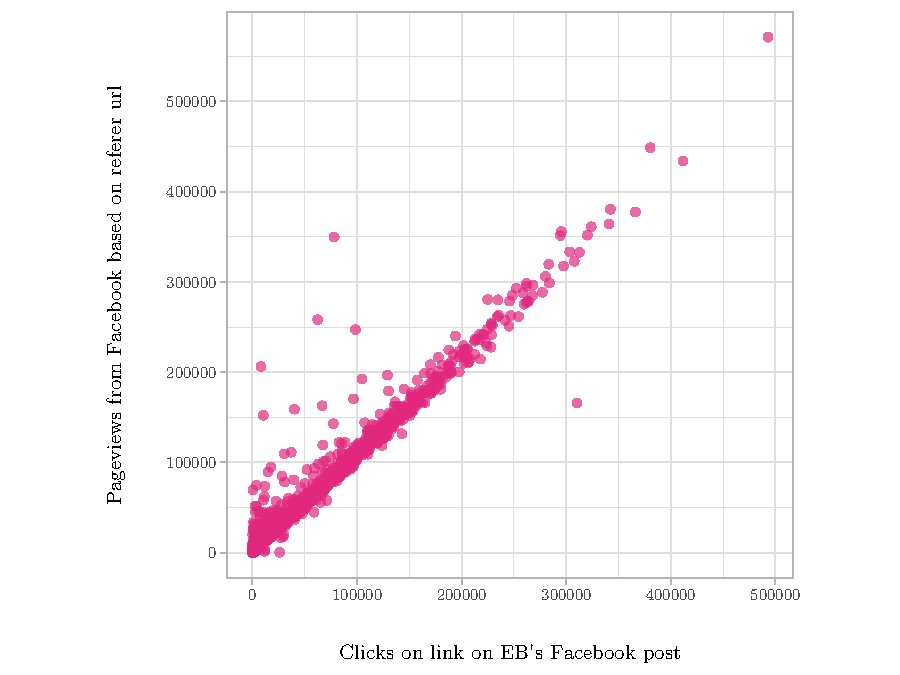
\includegraphics[width=300px,height=300px]{paper_files/figure-latex/sidneyplot-1} 

}

\caption{Scatterplot of Facebook pageviews and clicks on shared link}\label{fig:sidneyplot}
\end{figure}

\noindent As seen in Figure 9, only a few articles have a larger
proportion of pageviews to the article that does not come from the
shared link on Ekstra Bladet's Facebook page. There are also a few
articles that have more link clicks than pageviews of the article. The
reason for this is likely that users might click on the shared link, but
because of internet connection or server issues the request to the
article doesn't load -- thus not being registered on Ekstra Bladet's
website. There are a few articles that have almost twice the number of
link clicks than article pageviews. During the period, a few events have
caused quick, but massive spikes in pageviews on Ekstra Bladet's
website, which in a few cases has caused the website to be unable to
load correctly. These few outliers represent these cases - for example
the death of reality star Sidney Lee, and the heart attack of football
player Christian Eriksen.

Based on this measurement, we argue that most of the audience engagement
with the articles happens with and on the posts from Ekstra Bladet's own
Facebook page. There is of course also the question whether the observed
audience engagement can be generalized onto other audiences or other
social media than Facebook. However, this is a question of discussion
that we will return to in Section 5.4.

\hypertarget{conclusion-data-and-methods}{%
\subsection{Conclusion: Data and
Methods}\label{conclusion-data-and-methods}}

In this section, we describe the data and methods we employ in the study
to answer our research question. To bridge the two empirical limitations
from previous studies, this study uses a comprehensive dataset that we
were able to collect by collaborating with Ekstra Bladet -- the largest
Danish tabloid media. The dataset has two primary qualities
corresponding to each of the previously described limitations of
previous research. Instead of only relying on a sample of news content
that could suffer from unknown biases or missing representativity, we
are able to include the entire population of articles shared on Ekstra
Bladet's Facebook in almost a period of two years. The ability to
include the entire population of 18,350 shared articles is also
possible, because we utilize machine learning techniques rather than
manual hand-coding to label the news content characteristics. The second
quality of the dataset is that we are able to access a multitude of
features of audience engagement on Facebook by collaborating with Ekstra
Bladet. In this way, audience engagement is operationalized as a
multifaceted phenomenon with eight different empirical measurements of
four different dimensions of audience engagement on social media. To
analyze our research question, we employ eight multiple linear
regressions estimated with OLS and robust standard errors. In each of
the regression, our 11 predictors of news content characteristics are
included as well as five control variables mitigating confounding
effects of time, paywall access, and relevant consequential events such
as an election and an internal strategic change at Ekstra Bladet.
Finally, we consider some different important background factors,
including information about the demographic distribution, potential
selection bias, and Ekstra Bladet's strategies for engaging with
followers and moderating content.

\pagebreak

\hypertarget{analysis}{%
\section{Analysis}\label{analysis}}

In the following section, we present the answers to our research
question: \emph{``How does the content of news articles influence
audience engagement on social media?''}. As we discuss, there is a gap
within studies trying to answer this question, as most studies have
relied on small samples of shared news content which might suffer from
bias or non-representativity. Our study bridges this gap by including
all articles shared on Ekstra Bladet's Facebook page for one year and 10
months. In addition, very few studies have treated audience engagement
as a multifaceted phenomenon. Our study does not just operationalize
engagement as simple popularity cues, but incorporates several
dimensions of audience engagement including measures of informational
selection, emotional responses, sharing, and conversations around news
content. In this way, this study extends previous research by also
examining how different kinds of news content might result in different
kinds of audience engagement on social media. In the next sections, we
describe the results for each of the measures of audience engagement,
while discussing its theoretical implications.

\hypertarget{clicking-on-the-shared-link}{%
\subsection{Clicking on the Shared
Link}\label{clicking-on-the-shared-link}}

As described in Section 2.3.3., one dimension of audience engagement is
information selection, which we measure through the choice of clicking
on the news article shared in the post. In the Facebook post, the
audience is exposed to a snapshot of the article content in form of the
title, a picture, and an accompanying caption written specifically for
the Facebook post. In this way, clicking on the link to read the article
on the website of Ekstra Bladet might represent a selection by the user
of relevance based on the immediate exposure. Table 5 below shows
descriptive statistics for the number of link clicks on each post.

\begin{table}[H]

\caption{\label{tab:click_describe}Descriptive statistics}
\centering
\begin{tabular}[t]{llllllll}
\toprule
Variable & N & Mean & Std. Dev. & Min & Pctl. 25 & Pctl. 75 & Max\\
\midrule
Link clicks & 18,350 & 11,840 & 27,002 & 0 & 1,024 & 9,829 & 492,849\\
\bottomrule
\end{tabular}
\end{table}

\noindent As seen in Table 5, a link to the shared article on average
gets approximately 11,800 clicks. However, there is a very large
variance between the posts with the most and least clicks. The number of
clicks on the shared link ranges from zero to almost half a million
clicks, and the standard deviation is more than double as large as the
mean. The distribution is heavily skewed with the majority of posts
having a relatively small number of link clicks, while a minority of
posts get a very high number of link clicks. Table 6 below shows the
results of a regression of our predictors of news content on the number
of link clicks as the outcome.

\begin{table}[H]
\begin{center}
\begin{tabular}{l D{)}{)}{11)3}}
\toprule
 & \multicolumn{1}{c}{Link clicks} \\
\midrule
\textbf{Intercept}                         &                           \\
\quad Intercept                            & 13535 \;  (471)^{***}     \\
\textbf{Predictors}                        &                           \\
\quad Timeliness                           & 456 \;  (627)             \\
\quad Unexpectedness                       & 3957 \;  (806)^{***}      \\
\quad Geographical proximity               & -392 \;  (587)            \\
\quad Cultural proximity                   & -3281 \; (2528)           \\
\quad Personalization                      & -188 \; (2087)            \\
\quad Negativity (topic, ref. neutral)     & 374 \;  (471)             \\
\quad Negativity (style, ref. neutral)     & 1313 \;  (455)^{**}       \\
\quad Positivity (style, ref. neutral)     & -2340 \;  (786)^{**}      \\
\quad Impact                               & -2544 \;  (675)^{***}     \\
\quad Spreadability                        & -4353 \;  (590)^{***}     \\
\quad Hard News (ref. soft news)           & -5286 \;  (426)^{***}     \\
\textbf{Control variables}                 &                           \\
\quad Posted time PM (ref. AM)             & 245 \;  (399)             \\
\quad Posted time, weekend, (ref. weekday) & -346 \;  (450)            \\
\quad Pay-wall article                     & 4277 \; (3312)            \\
\quad Strategy Change                      & 5724 \;  (471)^{***}      \\
\quad Election Period                      & -4680 \; (1155)^{***}     \\
\midrule
Num. obs                                   & \multicolumn{1}{c}{18350} \\
R$^2$                                      & \multicolumn{1}{c}{0.02}  \\
Adj. R$^2$                                 & \multicolumn{1}{c}{0.02}  \\
\bottomrule
\multicolumn{2}{l}{\scriptsize{***p < 0.001; **p < 0.01; *p < 0.05}}
\end{tabular}
\caption{Linear regression model}
\label{table:coefficients}
\end{center}
\end{table}

\noindent As Table 6 shows, several news content characteristics
significantly influence the number of link clicks. The results show that
unexpectedness and negativity based on the style have a positive
influence on the number of link clicks, while positivity, impact,
spreadability, and hard news have a negative influence on the number of
link clicks.

The strongest positive influence on the behavior of clicking on the link
is if news content contains unexpectedness. These articles receive on
average almost \textasciitilde3,900 more likes than other articles. This
finding emphasizes that the audience information selection is highly
driven by curiosity -- when news content is framed as surprising or
sensational, audiences are stimulated by a need to know. To some extent,
this is in line with concepts such as ``click-bait''-style headings used
by many news organizations, but in particular tabloid news (Bazaco et
al.~2019).

The strongest negative influence on the behavior of link clicks is news
content that contains hard news rather than soft news. Articles about
hard news topics such as politics, economy, etc. receive on average
\textasciitilde5,300 fewer link clicks than articles with soft news
topics such as entertainment or lifestyle. Similarly, news content that
contains high impact -- identified as breaking news content -- is
associated with \textasciitilde2,500 fewer link clicks. This finding
suggests audiences more often choose to read lighter news content.

We also see that positivity of the article content is negatively related
to link clicks, indicating that news content with positivity on average
receives \textasciitilde2,300 fewer link clicks compared to neutral news
content. On the other hand, a negative framing seems to be associated
with a higher number of link clicks, but here the effect size is smaller
at \textasciitilde1,300 more clicks. This finding is in line with
previous research, providing further evidence for a form of negativity
bias, where more attention is paid towards content that has a negative
nature (Robertson et al.~2023). However, quite interesting and in
contrast to the framing of the articles, the content pertaining to
negative topics seem to have no significant impact on the number of link
clicks.

Finally, if the post contains spreadability, meaning that the
accompanying caption is framed as a question, it is negatively related
to link clicks, on average receiving \textasciitilde4,400 fewer clicks
on the article. This result falls in line with the argument of Jenkins
et al.~(2013) that content related to spreadability is perhaps not
directed at gaining attention from individuals, but rather to invoke
interpersonal behaviors.

The results are interesting in relation to previous literature on
seeking, selecting and obtaining knowledge from news content (See
Section 2.3.3.). Many previous studies have emphasized the importance of
news content in learning and gaining factual information in order to
have an informed democracy. As our results suggests that the audience
more often choose to read news content with soft news topics and news
content that is not breaking news, one might consider, if it is
problematic that the public prefers entertainment instead of reading
about heavier and important societal issues. Based on our results, the
behavior of selecting to read content might be more related to
entertainment or curiosity than gaining factual knowledge or learning
about societal conditions. This motivation of entertainment and
curiosity may be particularly tied to the media's tabloid style and
their audience. However, it is also important to note that we cannot
know from this empirical basis if the audience obtain the same knowledge
from softer or heavier topics, but we can only see that the softer
topics are more popular when controlling for the other types of news
content characteristics.

\hypertarget{emotional-responses-2}{%
\subsection{Emotional Responses}\label{emotional-responses-2}}

As described in Section 2.3.4., a behavior of audience engagement might
also be reacting to news content. While there may be different reasons
for reacting to a post, we argue that it could be seen as an emotional
response by the user. While an emotional reaction usually exists as a
feeling within the individual, it may be digital manifested as actual
behavior on Facebook, where it is possible to indicate your emotional
response to a post. We measure emotional responses as the sum of all
types of reactions, which might represent a general emotional valence.
Table 7 below shows descriptive statistics for this outcome of the
number of reactions.

\begin{table}[H]

\caption{\label{tab:react_describe}Descriptive statistics}
\centering
\begin{tabular}[t]{llllllll}
\toprule
Variable & N & Mean & Std. Dev. & Min & Pctl. 25 & Pctl. 75 & Max\\
\midrule
Number of reactions & 18,350 & 588 & 1,329 & 0 & 69 & 562 & 41,961\\
\bottomrule
\end{tabular}
\end{table}

\noindent A post receives on average 588 reactions. However, there is
also a large variation as the standard deviation is 1329, and the number
of reactions ranges from 0 to a maximum of 41961 reactions. This
indicates that the variable follows a power law distribution, where a
lot of the observations are distributed at the lower end, while a few
observations are far to the right creating a long tail to the right. The
75\%-percentile is 562 reactions, which interestingly enough is lower
than the mean of 588. Thus, 75\% of the posts have fewer than 562
reactions, while the remaining top 25\% has a much larger number of
reactions. Table 8 below shows the results of the regression of news
content on number of reactions as the outcome.

\begin{table}[H]
\begin{center}
\begin{tabular}{l D{)}{)}{9)3}}
\toprule
 & \multicolumn{1}{c}{Number of reactions} \\
\midrule
\textbf{Intercept}                         &                           \\
\quad Intercept                            & 470 \;  (23)^{***}        \\
\textbf{Predictors}                        &                           \\
\quad Timeliness                           & -2 \;  (31)               \\
\quad Unexpectedness                       & -54 \;  (40)              \\
\quad Geographical proximity               & 20 \;  (29)               \\
\quad Cultural proximity                   & -28 \; (124)              \\
\quad Personalization                      & 77 \; (103)               \\
\quad Negativity (topic, ref. neutral)     & -53 \;  (23)^{*}          \\
\quad Negativity (style, ref. neutral)     & -33 \;  (22)              \\
\quad Positivity (style, ref. neutral)     & 198 \;  (39)^{***}        \\
\quad Impact                               & 524 \;  (33)^{***}        \\
\quad Spreadability                        & -59 \;  (29)^{*}          \\
\quad Hard News (ref. soft news)           & 5 \;  (21)                \\
\textbf{Control variables}                 &                           \\
\quad Posted time PM (ref. AM)             & 36 \;  (20)               \\
\quad Posted time, weekend, (ref. weekday) & 10 \;  (22)               \\
\quad Pay-wall article                     & -343 \; (163)^{*}         \\
\quad Strategy Change                      & 246 \;  (23)^{***}        \\
\quad Election Period                      & -174 \;  (57)^{**}        \\
\midrule
Num. obs                                   & \multicolumn{1}{c}{18350} \\
R$^2$                                      & \multicolumn{1}{c}{0.02}  \\
Adj. R$^2$                                 & \multicolumn{1}{c}{0.02}  \\
\bottomrule
\multicolumn{2}{l}{\scriptsize{***p < 0.001; **p < 0.01; *p < 0.05}}
\end{tabular}
\caption{Linear regression model}
\label{table:coefficients}
\end{center}
\end{table}

\noindent As seen in Table 8, several news contents characteristics have
a significant influence on the number of reactions. The news content
characteristic of impact has the largest coefficient size, which shows
that impactful news content -- measured as breaking news -- receives
\textasciitilde500 more reactions than regular news content. Thus, news
content with high impact drives a higher emotional response. While
impact is negatively related to the behavior of clicking on the link
(see previous section), it is related to an increase in reactions. While
news content with high impact, such as breaking news, has a negative
influence on the number of people reading an article, it has a positive
influence on the number of emotional responses. From the perspective of
media's important role in an informed democracy, it might be problematic
that the audiences would rather read about soft news and low impact news
content, but as this result show, news content with high societal impact
on the other hand drives more emotional responses. The audience might
often choose to read news content for entertainment purposes, but high
impact content might still leave a stronger emotional impression on the
audience than other types of content.

In addition, Table 8 also shows that articles containing positivity
receive \textasciitilde200 more reactions than those with neutral
sentiment. On the other hand, articles with negativity defined by the
style receive 53 fewer reactions than neutral news content. In this way,
our results suggest that news content with positivity influences
audience reactions more than news content with negativity. In line with
the idea of emotional contagion, the emotional framing of the article
seems to influence the emotional response of the audience. However, the
results here are in contrast to the previous literature, as emotional
contagiousness can be seen for content containing a positive framing but
not for content containing a negative framing. Yet, it is important to
bear in mind that our aggregated measure of reactions captures the
general valence of the emotional response, and that more fine-grained
associations might be found for particular emotions such as negative
news leading to more negative reactions.

The results also show that news content characterized by spreadability
receives 59 fewer reactions. While having a smaller negative influence
than for link clicks, reacting may be seen as an individual form of
engagement and is as such not increased by the spreadability. None of
the remaining characteristics of news content have an influence on the
number of reactions.

The number of reactions, which has been used more commonly as a measure
of audience engagement, is not influenced by news content in the same
way as the number of link clicks was. Comparing the relation between the
news content characteristics and these two outcomes, it is clear that
the news content does not have a universal effect on audience engagement
on social media. In this way, these results emphasize that audience
engagement is a multifaceted phenomenon.

\hypertarget{sharing-1}{%
\subsection{Sharing}\label{sharing-1}}

In this section, we consider the dimension of audience engagement on
social media related to the behavior of sharing. As mentioned, we differ
between two different forms of sharing behaviors. The first is seen as a
way of sharing information through the implemented share button, which
allows a user to share the post to their own feed with the possibility
of adding their own accompanying text. The other is a more
interpersonal, targeted way of sharing measured through mention
comments. Where the first kind of sharing might relate to sharing for
social status or spreading information to one's entire network, the
latter is a way of sharing which is directed to a specific other person
that might be related to the idea of phatic news sharing. In Table 9
below, we show descriptive statistics for the two outcomes: number of
shares and proportion of mention comments.

\begin{table}[H]

\caption{\label{tab:share_describe}Descriptive statistics}
\centering
\begin{tabular}[t]{llllllll}
\toprule
Variable & N & Mean & Std. Dev. & Min & Pctl. 25 & Pctl. 75 & Max\\
\midrule
Number of shares & 18,350 & 25 & 61 & 0 & 2 & 23 & 1,879\\
Prop. of mention comments & 18,350 & 0.065 & 0.097 & 0 & 0.0067 & 0.081 & 1\\
\bottomrule
\end{tabular}
\end{table}

\noindent From Table 9, we see that a post is shared on average
\textasciitilde25 times. However, there is also a large variation among
the posts, where the standard deviation is \textasciitilde61 ranging
from a post being shared between 0 times and a maximum of 1879 times. In
the comment sections of the posts, there is 6.5\% mention comments on
average. For the proportion of mention comments, there is also a large
standard deviation of 9.7\%-points. While some posts do not have any
mention comments, other posts have only mention comments. Table 10 below
shows the result of news content on the two outcomes of sharing.

\begin{table}[H]
\begin{center}
\begin{tabular}{l D{)}{)}{11)3} D{)}{)}{11)3}}
\toprule
 & \multicolumn{1}{c}{Number of shares} & \multicolumn{1}{c}{Prop. of mention comments} \\
\midrule
\textbf{Intercept}                         &                           &                           \\
\quad Intercept                            & 16 \; (1.059)^{***}   & 0.068 \; (0.002)^{***}    \\
\textbf{Predictors}                        &                           &                           \\
\quad Timeliness                           & 2 \; (1.411)          & 0.008 \; (0.002)^{***}    \\
\quad Unexpectedness                       & -1 \; (1.813)         & 0.001 \; (0.003)          \\
\quad Geographical proximity               & 2 \; (1.320)          & 0.011 \; (0.002)^{***}    \\
\quad Cultural proximity                   & -4 \; (5.687)         & -0.009 \; (0.009)         \\
\quad Personalization                      & -7 \; (4.694)         & -0.033 \; (0.008)^{***}   \\
\quad Negativity (topic, ref. neutral)     & -7 \; (1.059)^{***}   & 0.008 \; (0.002)^{***}    \\
\quad Negativity (style, ref. neutral)     & -1 \; (1.024)         & -0.017 \; (0.002)^{***}   \\
\quad Positivity (style, ref. neutral)     & -7 \; (1.767)^{***}   & 0.008 \; (0.003)^{**}     \\
\quad Impact                               & 6 \; (1.517)^{***}    & -0.013 \; (0.002)^{***}   \\
\quad Spreadability                        & -1 \; (1.326)         & -0.001 \; (0.002)         \\
\quad Hard News (ref. soft news)           & 19 \; (0.957)^{***}   & -0.003 \; (0.002)^{*}     \\
\textbf{Control variables}                 &                           &                           \\
\quad Posted time PM (ref. AM)             & 0 \; (0.897)          & -0.001 \; (0.001)         \\
\quad Posted time, weekend, (ref. weekday) & -3 \; (1.012)^{**}    & -0.005 \; (0.002)^{**}    \\
\quad Pay-wall article                     & -7 \; (7.450)         & 0.014 \; (0.012)          \\
\quad Strategy Change                      & 4 \; (1.060)^{***}    & 0.006 \; (0.002)^{***}    \\
\quad Election Period                      & -4 \; (2.597)         & -0.000 \; (0.004)         \\
\midrule
Num. obs                                   & \multicolumn{1}{c}{18350} & \multicolumn{1}{c}{18350} \\
R$^2$                                      & \multicolumn{1}{c}{0.03}  & \multicolumn{1}{c}{0.01}  \\
Adj. R$^2$                                 & \multicolumn{1}{c}{0.03}  & \multicolumn{1}{c}{0.01}  \\
\bottomrule
\multicolumn{3}{l}{\scriptsize{***p < 0.001; **p < 0.01; *p < 0.05}}
\end{tabular}
\caption{Linear regression models}
\label{table:coefficients}
\end{center}
\end{table}

\noindent As Table 10 shows, two different news content characteristics,
hard news and impact, have a positive impact on the number of shares --
measured as sharing to your entire social network. News content with
hard news topics has the largest influence on the number of shares.
Those articles on average receive \textasciitilde19 more shares than
articles with soft news. Furthermore, news content with high impact
measured as breaking news is on average shared \textasciitilde6 more
times. These findings indicate that sharing to your entire social
network might be important for your social status, and that the
audiences find societal relevance important when considering what kind
of news content, they want to be associated with (Thompson et al.~2020;
See also Section 2.3.5). It is possible that users who share news
content to their entire social network see themselves as a kind of
opinion leaders that distribute and curate the most important news to
their network (See Section 2.1.2). However, we do not know the specific
motivations for the users who share, but only that they tend to share
more news content with impact and hard news topics.

On the other hand, some types of news content have a negative influence
on the number of shares. News content with negativity based on topic
gains \textasciitilde7 fewer shares, while news content with positivity
based on style also receives \textasciitilde7 fewer shares, compared to
news content with neutral sentiment. Interestingly, news content with
negativity based on the style is not significantly different than those
with neutral sentiment in regard to the number of shares. Nonetheless,
this kind of sharing seems to be negatively influenced by emotionally
laden news content. Following the idea that this type of engagement is
related to social status, an explanation might be that those who spread
news content do not wish to be associated with emotionally laden
content.

The rest of the news content characteristics (timeliness,
unexpectedness, geographical and cultural proximity, personalization,
and spreadability) have no significant impact on the number of shares.
The fact that spreadability -- identified as news content framed as a
question -- is not associated with a higher number of shares may be
because of the way people wish to associate and engage with the specific
content. Here people are perhaps looking to spread a specific piece of
information, pose their own questions, or frame it in their own way, all
actions which may be less relevant if the original post is already
framed with a specific question. This finding goes against the argument
by Jenkins et al.~(2013) about spreadability leading to more sharing of
the content.

\hspace{-2.5em}

\noindent For the other outcome of sharing -- the proportion of mention
comments -- Table 10 shows quite different results than for the number
of shares. The coefficients for the proportions represent differences in
percentage points and are all rather low, and as such we are not able to
explain much of the present variance. However, looking at the news
content characteristics, the highest positive influence on the
proportion of mention comments is geographical proximity. On average,
news content with geographic proximity has a 1.1\%-points larger
proportion of mention comments. Individuals residing in the same
geographic area as the news story -- here identified as any location
within Denmark -- may possess more familiarity and understanding of the
local context, making them more likely to activate social ties through
mention comments. Geographical closeness is often common between friends
-- people tend to live near their social network -- and this might
explain that geographical markers influence this directed, interpersonal
kind of sharing (Almquist 2016). The news content characteristics of
timeliness and negativity based on the topic also have a significant
positive influence on the proportion of mention comments, but the effect
sizes only show a 0.8\%-points larger proportion of mention comments.

As Table 10 shows, there are also several news content characteristics
that have a negative influence on the proportion of mention comments.
News content with personalization has the largest negative influence on
the proportion of mention comments. On average, news content with
personalization -- measured if the title or subtitle of the article
contains a named person -- receives -3.3\%-points smaller proportion of
mention comments. As outlined in Section 3.3.1., our measure of
personalization mostly captures names of famous people such as
politicians, professional athletes, or other celebrities. Thus, having a
focus on elite persons in the article seems to be something that is not
used to activate or maintain social ties to a larger degree.

The news content characteristic of impact also has a significant
negative influence on the proportion of mention comments. This kind of
news content receives -1.3\%-points smaller proportion of mention
comments. Compared with the other kind of sharing, news content with
impact influences a higher number of shares to your entire social
network, but a lower proportion of mentions comments. An explanation of
this could be that news content with high societal impact might drive a
need for sharing with your entire social network rather than just one
specific social tie.

News content with positivity and negativity based on the topic on
average gain 0.8\%-points more mentions comments, which is a rather
small difference. News content with negativity based on the style gain
-1.7\%-points smaller proportion than the neutral ones. As the effect
size for positivity and negativity based on the topic is smaller than
1\%-points, the results suggest that emotionally laden news content,
both positive and negative, generally seems to decrease or not really
influence sharing behavior. Here, the results show some similarity to
the first kind of sharing, where emotional valence of the news content
also has a negative influence. In this way, the positivity and
negativity of the news content seems to decrease both sharing towards
your entire social network and directed, interpersonal sharing.

\hspace{-2.5em}

\noindent In conclusion, there are noticeable differences between the
two outcomes of sharing behavior included in the analysis. News content
with impact increases sharing with your entire social network, while
having a negative influence on the interpersonal sharing. Geographical
proximity increases the latter but does not have an influence on the
former. Furthermore, emotionally laden news content, both positive and
negative, seems to have a negative or no influence of both types of
sharing.

\hypertarget{conversations}{%
\subsection{Conversations}\label{conversations}}

As described in Section 3.3.1., the dimension of audience engagement
related to having conversations about news content is measured by four
different outcomes representing the volume, reciprocity, respect, and
disrespect of the conversations. The following section consists of two
parts. The first part analyzes the volume and reciprocity of the
conversation, while the second part analyzes the respect and disrespect
measured by recognizing and offensive language.

\hypertarget{volume-and-reciprocity}{%
\subsubsection{Volume and Reciprocity}\label{volume-and-reciprocity}}

\noindent In this section, we examine the results for two outcomes of
how the audience engages in conversations about the news content: the
volume of conversation measured by the number of comments, and the
reciprocity of the conversation measured by the proportion of reply
comments out of all comments. The first represent a general volume of
comments and conversations, while the second relates to the depth of the
conversations -- whether audiences enter in dialogue rather than one-way
utterances. Table 11 below shows descriptive statistics for these two
outcomes.

\begin{table}[H]

\caption{\label{tab:comment_describe}Descriptive statistics}
\centering
\begin{tabular}[t]{llllllll}
\toprule
Variable & N & Mean & Std. Dev. & Min & Pctl. 25 & Pctl. 75 & Max\\
\midrule
Number of comments & 18,350 & 289 & 589 & 1 & 31 & 313 & 17,327\\
Prop. of reply comments & 18,350 & 0.43 & 0.19 & 0 & 0.31 & 0.57 & 0.97\\
\bottomrule
\end{tabular}
\end{table}

\noindent As seen in Table 11, both of these outcomes have a large
variance as number of comments ranges from 1 comment to 17,327 comments
on a post, and the proportion of reply comments ranges from 0\% to 97\%.
On average, the posts in our dataset receive 289 comments, where approx.
43\% are reply comments, i.e., comments on another comment. In Table 12
below, we present the results of the regressions of news content on each
of these two outcomes.

\begin{table}[H]
\begin{center}
\begin{tabular}{l D{)}{)}{14)3} D{)}{)}{11)3}}
\toprule
 & \multicolumn{1}{c}{Number of comments} & \multicolumn{1}{c}{Prop. of reply comments} \\
\midrule
\textbf{Intercept}                         &                            &                           \\
\quad Intercept                            & 209 \; (10.183)^{***}  & 0.379 \; (0.003)^{***}    \\
\textbf{Predictors}                        &                            &                           \\
\quad Timeliness                           & 22 \; (13.568)         & 0.003 \; (0.004)          \\
\quad Unexpectedness                       & -33 \; (17.436)        & -0.015 \; (0.006)^{**}    \\
\quad Geographical proximity               & -1 \; (12.699)         & -0.005 \; (0.004)         \\
\quad Cultural proximity                   & -28 \; (54.696)        & -0.008 \; (0.018)         \\
\quad Personalization                      & -9 \; (45.148)         & 0.014 \; (0.015)          \\
\quad Negativity (topic, ref. neutral)     & -133 \; (10.183)^{***} & 0.018 \; (0.003)^{***}    \\
\quad Negativity (style, ref. neutral)     & 28 \;  (9.844)^{**}    & 0.005 \; (0.003)          \\
\quad Positivity (style, ref. neutral)     & -61 \; (16.995)^{***}  & -0.034 \; (0.005)^{***}   \\
\quad Impact                               & 106 \; (14.591)^{***}  & 0.005 \; (0.005)          \\
\quad Spreadability                        & 138 \; (12.756)^{***}  & -0.027 \; (0.004)^{***}   \\
\quad Hard News (ref. soft news)           & 134 \;  (9.209)^{***}  & 0.089 \; (0.003)^{***}    \\
\textbf{Control variables}                 &                            &                           \\
\quad Posted time PM (ref. AM)             & -7 \;  (8.629)         & -0.003 \; (0.003)         \\
\quad Posted time, weekend, (ref. weekday) & -58 \;  (9.734)^{***}  & -0.007 \; (0.003)^{*}     \\
\quad Pay-wall article                     & -12 \; (71.649)        & 0.012 \; (0.023)          \\
\quad Strategy Change                      & 127 \; (10.194)^{***}  & 0.036 \; (0.003)^{***}    \\
\quad Election Period                      & -34 \; (24.978)        & 0.009 \; (0.008)          \\
\midrule
Num. obs                                   & \multicolumn{1}{c}{18350}  & \multicolumn{1}{c}{18350} \\
R$^2$                                      & \multicolumn{1}{c}{0.04}   & \multicolumn{1}{c}{0.08}  \\
Adj. R$^2$                                 & \multicolumn{1}{c}{0.04}   & \multicolumn{1}{c}{0.08}  \\
\bottomrule
\multicolumn{3}{l}{\scriptsize{***p < 0.001; **p < 0.01; *p < 0.05}}
\end{tabular}
\caption{Linear regression models}
\label{table:coefficients}
\end{center}
\end{table}

\noindent As Table 12 shows, there are several of the news content
characteristics that have a significant influence on the two outcomes.
For the first outcome, number of comments, both negativity based on
style, impact measured as breaking news, spreadability, and hard news
content seems to have a positive relationship with the number of
comments. Moreover, unexpectedness, negativity based on the topic, and
positivity have a significant negative influence on the number of
comments. For the second outcome, the proportion of reply comments, both
negativity based on the topic, hard news topic seems to have a positive
influence, while unexpectedness, positivity, and spreadability has a
negative influence.

Specifically, news content about hard news topics such as politics and
economy on average receives \textasciitilde130 more comments compared to
soft news topics. Furthermore, news content about hard news topics also
has on average 8.8\%-points larger proportion of reply comments than
news content with soft news topics. Interestingly, the audience
engagement of commenting on the post seems to be very differently
related to the news content characteristics compared to the behavior of
clicking on the link to read the article (See Section 4.1.). While the
news content characteristics of hard news topics and impact were
negatively related to link clicks, they were positively related to
number of shares, and also positively related to number of comments.
This result might indicate that the behaviors of link clicking and
commenting are related to different kinds of motivations for audience
engagement. News content with soft topics and with less societal impact
might drive more link clicks as they serve purposes of entertainment and
individual information selection, while news content with hard news
topics and with high societal impact drive an urge to express opinions
and have dialogues with other members of the audience. Related to the
idea of deliberative democracy, we argue that it is valuable that news
content with high societal relevance also seems to stimulate more public
conversations and fosters more reciprocity, which are important forms of
participation in an informed public sphere.

In addition, the results for news content with negativity and positivity
show that the volume and reciprocity of conversations might be related
to different kind of motivations for the specific behavior. Negativity
based on the topic -- e.g., if the article is about war, disasters, or
crime -- is negatively related to the volume of comments, but positively
related to the proportion of reply comments. Thus, news content with
negative topics influences less conversations, but a higher degree of
reciprocity and dialogue between the audiences engaging in the
conversation. On the other hand, news content with positivity drives
both less volume of conversations, and less reciprocity in the
conversations. The results also show a difference between negativity
based on the topic and negativity based on the style of the content, as
the latter is only slightly or not related to volume and reciprocity of
conversations.

Another interesting result is that spreadability is positively related
to the number of comments, but negatively related to the proportion of
reply comments. Particularly, a post with the accompanying caption
framed as a question on average receives 138 more comments, but
2.7\%-points smaller proportion of reply comments than other captions.
While the spreadability is not related to either link clicks, number of
shares, or proportion of mention comments, it seems to drive more
comments to the post. However, while spreadability drives a larger
volume of comments directly to the posts, it decreases the behavior of
engaging in dialogue, as it is negatively related to the proportion of
reply comments. The idea of spreadability has been emphasized especially
by Jenkins et al.~(2013), who argued that news content should be
designed to optimize spreadability. However, our results indicate that
spreadability only drives the volume of comments and less reciprocity of
comments, and therefore spreadability might not be a universally
effective way of optimizing the framing of news content.

\hypertarget{respect-and-disrespect}{%
\subsubsection{Respect and Disrespect}\label{respect-and-disrespect}}

\noindent In this section, we analyze the results for the next two
outcomes of how audiences engage in conversations: the disrespect
measured by the proportion of comments with offensive language and
respect measured by the proportion of comments with recognizing
language. Both of these engagement characteristics are important, as
they particularly relate to the quality of conversations. As described
in Section 2.3.6., the theoretical idea of deliberative democracy highly
emphasizes respect as a prerequisite for a good democratic debate around
news content. Table 13 below shows descriptive statistics for both of
these outcomes.

\begin{table}[H]

\caption{\label{tab:hate_describe}Descriptive statistics}
\centering
\begin{tabular}[t]{llllllll}
\toprule
Variable & N & Mean & Std. Dev. & Min & Pctl. 25 & Pctl. 75 & Max\\
\midrule
Prop. of offensive comments & 18,350 & 0.064 & 0.069 & 0 & 0.014 & 0.095 & 1\\
Prop. of recognizing comments & 18,350 & 0.12 & 0.12 & 0 & 0.061 & 0.14 & 1\\
\bottomrule
\end{tabular}
\end{table}

\noindent As Table 13 shows, the average proportion of offensive
comments in a comment section is at 6.4\%, with a standard deviation of
6.9\%-points, a min of 0\% and a max of 1\%. The average proportion of
comments containing recognizing language is 12.1\%, with a standard
deviation of 12.3\%-points and a min of 0\% and a max of 1\%. Compared
to the average of other nation-wide Danish media, Ekstra Bladet on
average has a lower proportion of recognizing comments (12.1\% compared
to 13-15\%) and a slightly higher proportion of offensive comments
(6.4\% compared to 5\%) (Analyse \& Tal 2021a; Analyse \& Tal 2021b).
Table 14 below presents the results of the regression of news content
characteristics on the outcomes representing disrespect and respect.

\begin{table}[H]
\begin{center}
\begin{tabular}{l D{)}{)}{11)3} D{)}{)}{11)3}}
\toprule
 & \multicolumn{1}{c}{Prop. of offensive comments} & \multicolumn{1}{c}{Prop. of recognizing comments} \\
\midrule
\textbf{Intercept}                         &                           &                           \\
\quad Intercept                            & 0.044 \; (0.001)^{***}    & 0.149 \; (0.002)^{***}    \\
\textbf{Predictors}                        &                           &                           \\
\quad Timeliness                           & -0.003 \; (0.002)^{*}     & 0.003 \; (0.003)          \\
\quad Unexpectedness                       & 0.003 \; (0.002)          & -0.003 \; (0.004)         \\
\quad Geographical proximity               & -0.005 \; (0.001)^{**}    & 0.002 \; (0.003)          \\
\quad Cultural proximity                   & -0.004 \; (0.006)         & -0.008 \; (0.011)         \\
\quad Personalization                      & 0.023 \; (0.005)^{***}    & 0.017 \; (0.009)          \\
\quad Negativity (topic, ref. neutral)     & 0.030 \; (0.001)^{***}    & -0.007 \; (0.002)^{***}   \\
\quad Negativity (style, ref. neutral)     & 0.016 \; (0.001)^{***}    & -0.014 \; (0.002)^{***}   \\
\quad Positivity (style, ref. neutral)     & -0.013 \; (0.002)^{***}   & 0.040 \; (0.003)^{***}    \\
\quad Impact                               & 0.008 \; (0.002)^{***}    & 0.040 \; (0.003)^{***}    \\
\quad Spreadability                        & -0.009 \; (0.001)^{***}   & -0.032 \; (0.003)^{***}   \\
\quad Hard News (ref. soft news)           & 0.021 \; (0.001)^{***}    & -0.051 \; (0.002)^{***}   \\
\textbf{Control variables}                 &                           &                           \\
\quad Posted time PM (ref. AM)             & 0.001 \; (0.001)          & 0.000 \; (0.002)          \\
\quad Posted time, weekend, (ref. weekday) & -0.004 \; (0.001)^{***}   & 0.013 \; (0.002)^{***}    \\
\quad Pay-wall article                     & 0.012 \; (0.008)          & -0.022 \; (0.015)         \\
\quad Strategy Change                      & -0.003 \; (0.001)^{*}     & -0.003 \; (0.002)         \\
\quad Election Period                      & 0.002 \; (0.003)          & -0.005 \; (0.005)         \\
\midrule
Num. obs                                   & \multicolumn{1}{c}{18350} & \multicolumn{1}{c}{18350} \\
R$^2$                                      & \multicolumn{1}{c}{0.11}  & \multicolumn{1}{c}{0.08}  \\
Adj. R$^2$                                 & \multicolumn{1}{c}{0.11}  & \multicolumn{1}{c}{0.07}  \\
\bottomrule
\multicolumn{3}{l}{\scriptsize{***p < 0.001; **p < 0.01; *p < 0.05}}
\end{tabular}
\caption{Linear regression models}
\label{table:coefficients}
\end{center}
\end{table}

\noindent As Table 14 shows, almost all news content characteristics -
except unexpectedness and cultural proximity - have an either positive
or negative influence on the proportion of comments containing offensive
language. For the proportion of comments with recognizing language, news
content with negativity, spreadability, and hard news topic have a
negative influence, while news content with positivity or high impact
such as breaking news have a positive influence.

As the results in Table 14 show, news content with hard news topics on
average has 2.1\%-points larger proportions of comments containing
offensive language. This is similar to the findings for previous
research such as Coe et al.~(2014) (See Section 2.3.6.). However, we are
also able to add to this, as our results also show that news content
with hard news topic has a 5.1\%-points lower proportion of recognizing
comments than soft news topics. The theoretical explanation may be that
when the topic of discussion is of high societal importance, the
discussion might also be more passionate and heated, which may have
people turn to both offensive language and recognizing language rather
than neutral language. Considering the topics constituting hard news,
those articles may be more about political sensitive subjects such as
immigration, religion, or ideology, which may have a negative impact on
the tone (Coe et al.~2014).

In addition, the results in Table 14 show that news content with
negativity based on the topic receives 3\%-points larger proportion of
comments with offensive language. Similarly, news content with
negativity based on the style of the content receives 1.6\%-points
larger proportion of comments with offensive language. Furthermore, news
content with positivity receives -1.3\%-points smaller proportion of
offensive comments. The exact reverse relationship is found for the
proportion of comments with recognizing language. Here, news content
with negativity receives -0.7\%- and -1.4\%-points smaller proportion of
comments containing recognizing language, while news content with
positivity receives 4\%-points more comments with recognizing language.
While some of these coefficients are quite small, they do indicate the
presence of emotional contagion, i.e., that the emotional responses
among the audiences tend to be similar to the emotions encoded in the
news content (See Section 2.3.4.). In this way, the results also
reinforce the importance of the media in shaping the public debate, as
negativity or positivity compared to more neutral framings of the news
content seems to drive more or less respectful conversations about the
news content. This question is further discussed in Section 5.1.

Another characteristic of news content that influences more comments
with offensive language is personalization. When news content contains
personalization -- i.e., that there is a distinct focus on named persons
-- the conversation contains on average 2.3\%-points larger proportion
of comments with offensive language. As Coe et al.~(2014:673) have
suggested, an explanation of this mechanism could be that
personalization creates partisan cues. In other words, the focus on
elite actors in the news content might drive a division between
proponents and opponents of said person, and that these dynamics
increase incivility and disrespectful language.

The results also show that news content with impact influences a larger
proportion of offensive comments. News content with high impact measured
as breaking news in average receives a 0.8\%-points larger proportion of
comments with offensive language. However, the same kind of news content
also receives a 4\%-points larger proportion of comments with
recognizing language. Thus, independently of other news content
characteristics, news content with high societal relevance and impact
influences both a more disrespectful and respectful conversation. While
at first, this may seem paradoxical, it is important to note that the
two characteristics are not mutually exclusive, but the reference
category is a neutral conversation. An example to explain such as case
from our data is three breaking news articles about the kidnapping and
murder of a 22-year-old woman in the beginning of February 2022 . This
story exemplifies news content that is both tragic and infuriating, and
thus might influence the audience to both express empathy as well as
anger towards the news content. Other kinds of such examples from our
data include articles about the death of famous persons and victories or
losses in sports events, which might influence both kinds of audience
engagement.

Finally, news content containing spreadability drives a -0.9\%-points
smaller proportion of comments with offensive language as well as a
-3.2\%-points smaller proportion of comments with recognizing language.
Recalling the results from Section 4.4., spreadability leads to a higher
volume of conversations, but less reciprocity and also less offensive
and recognizing language. This further supports the interpretation that
spreadability only drives more conversations, but not necessarily more
elaborate conversations or emotionally laden responses.

\hypertarget{conclusion-analysis}{%
\subsection{Conclusion: Analysis}\label{conclusion-analysis}}

In the previous sections, we present the results of our analysis. As our
analysis entails eight different outcomes and 11 predictors, we focus on
the significant coefficients, since a full review of all coefficients
and control variables is too extensive for the scope of this study.
Figure 10 below, shows all significant coefficients, color-scaled to
show the most impactful coefficients.

\begin{figure}[H]

{\centering 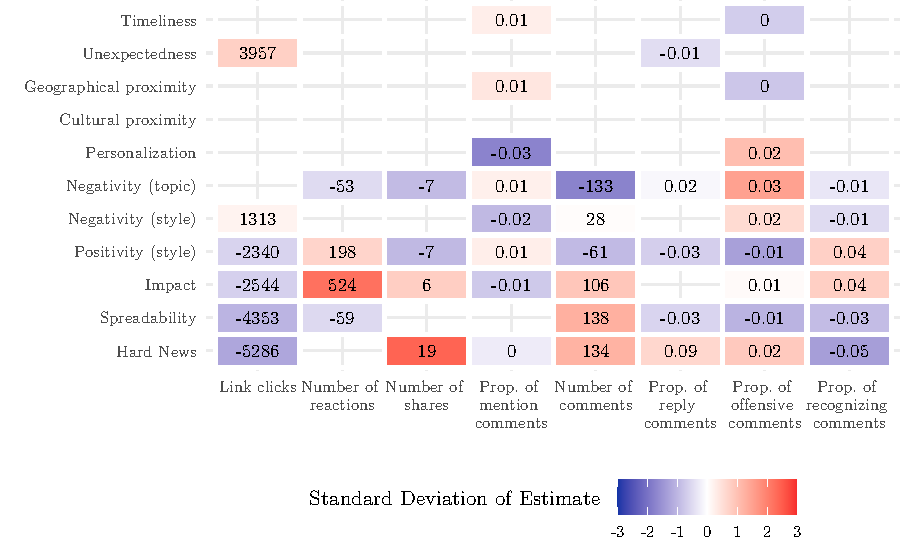
\includegraphics[width=0.8\linewidth]{paper_files/figure-latex/coef_matrix-1} 

}

\caption{Summary of regression models}\label{fig:coef_matrix}
\end{figure}

\begin{center}
\small
Each column represents a regression model. Only coefficients with a p-value < 0.05 are shown. For each model, the color corresponds to how many standard deviations the coefficient is from zero.
\end{center}
\normalsize

\noindent The analysis seeks to answer the research question:
\emph{``How does the content of news articles influence audience
engagement on social media?''}. As our results have shown, the content
of news articles does indeed impact the audience engagement on Facebook.
However, it is also clear that the effect of news content varies greatly
across different kinds of audience engagement behavior. News content
might drive more of a certain behavior, while driving less of another
behavior. Summarizing across the results from the regressions, we argue
that there are three main findings of our analysis: 1) soft news and
unexpectedness drive individualistic behavior, while news content with
larger societal relevance drives more social behavior, and 2) the
sentiment of the news content drives a similar sentiment in audience
discussions, and 3) timeliness and proximity have no or only small
effects on any kind of audience engagement.

First of all, news content with unexpectedness and soft news topics
influences individualistic audience engagement such as clicking on the
link to read the article, whereas news content that holds greater
societal relevance encourages more social audience engagement such as
sharing or having conversations around the news content. The news
content characteristics with the largest positive influence on the
behavior of clicking on the link is unexpectedness, while the largest
negative influences are hard news topic, spreadability and impact. On
the contrary, news content with impact or hard news topics generally
gains more comments and a larger proportion of reply comments compared
with soft news or not breaking news content. In conclusion, these
results suggest that articles about soft news or unexpectedness lead to
more individualistic audience engagement in form of link clicks, which
might represent a motivation for curiosity or entertainment rather than
a motivation of having deeper social interactions and deliberations
among the audience members. On the other hand, the results also suggest
that articles of larger societal relevance such as impact or hard news
topics are associated with more social audience engagement such as
sharing and discussions on the comment section.

Secondly, the results show that the negativity or positivity also
influences the negativity or positivity in the audience engagement in
the comment sections. Thus, a negative sentiment in the article drives a
larger proportion of comments with offensive language and a smaller
proportion of comments with recognizing language, while a positive
sentiment in the article drives a smaller proportion of comments with
offensive language and a larger proportion of comment with recognizing
language. While hard news leads to more conversation volume and
reciprocity, the results also show that hard news are associated with a
larger proportion of comments with offensive language, and a smaller
proportion of comments containing recognizing language. As such, the
presence of substantial and political issues often comes with the price
of increased incivility. We also find that positive news content and
especially impactful news content increase the volume of emotional
valence as measured by aggregated reactions, however the association is
not found for negative news content. Nonetheless, we argue that the
findings about negativity and positivity can generally be tied to the
idea of emotional contagion; the emotional framing and content of an
article may influence the emotional responses of the audience.

Finally, across all outcomes of audience engagement, the results show
mostly small or no effects of timeliness and proximity (both cultural
and geographical). These predictors are only significantly associated
with the proportion of mention comments and proportion of offensive
comments, but the effect sizes are rather small. At first, the
conclusion of this might be that these news content characteristics do
not have an effect on the audience engagement when controlled for other
news content characteristics. However, there might also be
methodological limitations behind these findings, which we discuss
further in Section 5.3.1 for proximity and in Section 5.4. for
timeliness.

Concluding on these results, our most essential finding is that the
characteristics of news content do not have a universal influence on
audience engagement. Based on news value theory, previous studies and
literature have primarily expected an increase in audience engagement
for any of the news content characteristics. Nonetheless, our findings
show that news content characteristics might not have an effect on all
dimensions of audience engagement, and they might even decrease specific
kinds of audience engagement. This contributes to an understanding of
audience engagement as a multifaceted phenomenon, which may be affected
in heterogeneous ways by different kinds of news content.

\pagebreak

\hypertarget{discussion}{%
\section{Discussion}\label{discussion}}

In the previous section, we presented our results in order to answer our
research question. In this section, we discuss the implications that
these findings may entail, the limitations of the analysis, as well as
future directions. First of all, we discuss societal implications in
terms of the pivotal democratic role of news media facilitating public,
political discussions. Secondly, we argue that the findings point
towards a further theorization about what causal mechanisms that drive
the heterogenous effects of news content on audience engagement that we
identified in our empirical analysis. Subsequently, the reliability of
the measured effects is discussed, especially in relation to the
concerns of granularity, context, and algorithmic confounding. Finally,
we also consider how our findings might generalize to other contexts.

\hypertarget{societal-implications}{%
\subsection{Societal Implications}\label{societal-implications}}

As mentioned in Section 1.1., the Facebook pages and comment sections of
Danish news media have been extensively discussed in recent years.
Social media like Facebook have been praised for providing the audience
with more agency, as they facilitate new possibilities for discussing
and deliberating news content. On the other hand, the comment sections
on social media like Facebook have also been notorious for uncivil
language and possessing qualities opposite of constructive deliberation
as imagined by sociologists like Habermas (See Section 2.3.6.).
Recently, the solution to poor conversation quality around news content
on social media have been to shut down the ability to comment (Reimer et
al.~2021:4). At first sight, the shutdown of comment sections might be
an effective and cheap solution, as it removes the possibility for
negative content while also removing the otherwise necessary expenses
for content moderators. On the other hand, removing the public debate in
itself may be damaging from a societal and democratic perspective. If
news media do not provide a public space for citizens to engage and
discuss important societal issues, it might erode the potential for all
voices to be heard and damage the legitimacy of democratic processes.
Furthermore, removing the ability to comment may limit the exposure of
news content -- thus neglecting the obligation of news media in an
informed democracy. Therefore, it is crucial to find ways of promoting
sustainable public conversations around news content on social media
rather than just removing the possibility for discussion entirely.

The results of this study indicate how certain types of news content
might yield a more constructive deliberation than other types of news
content. Our analysis found that news content with hard news topics and
high impact sparked a higher volume and reciprocity of conversations
among the audience, but it also resulted in more offensive language.
Furthermore, the emotional framing of the news content also resulted in
more emotional responses among the audience, and thus negativity also
sparked more offensive language in the comment sections. In this way,
the journalistic framing of the news content seems to influence how the
deliberation unfolds in Facebook's comment sections. To promote better
deliberation, it is worth considering whether news content can be framed
in a way that encourages more volume and reciprocity without incivility
in online conversations. For example, our results suggest that it might
be good to avoid negative framings of news content, as negativity drives
uncivil conversations in the Facebook comment sections. For the hard
news topic that also yields a higher volume and reciprocity of
conversations, increased focus on moderation may be a necessity.

A challenge here might be that media organizations also have an economic
motivation for their journalistic framing of news content. The source of
revenue for all media companies -- whether their economic model is
ad-based or subscription-based -- is to generate link clicks in order to
move audiences from Facebook to the media's own website (Martin 2019).
At a societal level, not only the quantity but also the quality of
engagement may be important for providing a space for public political
deliberation. As an example, studies have shown that uncivil comments
may decrease the perceived legitimacy of the news content and media
(Houston 2011; Kümpel \& Springer 2016; Gearhart et al.~2022).
Furthermore, our results indicate that the types of news content that
influences more link clicks is not the same news content that influences
more social behavior among the audience such as sharing and commenting.
Therefore, media organizations might have to strike a balance between
optimizing their content for engagement quantity to increase revenue and
engagement quality to increase deliberation and social behavior.

\hypertarget{theoretical-future-directions}{%
\subsection{Theoretical Future
Directions}\label{theoretical-future-directions}}

From the results of our empirical analysis, a central finding is that
news content does not have a universal effect on audience engagement.
Instead, news content has varying effects on different dimensions of
audience engagement behavior. Following this finding, the question
follows: what then is the theoretical explanation of how a specific news
content characteristic drives either more or less of a specific
dimension of audience engagement? The present study is only based on
correlational evidence, so in order to determine the validity of the
study it is important to have a strong theoretical argument about the
mechanism that drives the identified correlations (See Section 3.4.2.).

Many of the studies reviewed provided only vague descriptions about the
underlying causal mechanisms, while others mainly draw on psychological
concepts. In many studies, the objective seems to be simply to explain
the digital traces on Facebook as an outcome in itself, instead of
considering the digital trace behavior as a manifestation of underlying
social mechanisms. We argue that our approach of supplementing with
sociological theories may help gain a more comprehensive understanding
of what drives the influence of news content on audience engagement.
This includes both grand theories of deliberation and communicative
action (i.e., Habermas), but also more micro level theories about
reciprocity and social cohesion (e.g., Mauss). However, the inquiry of
our study has been mainly empirical, and therefore we have not tried to
actively develop the theories of audience engagement and news content.
To do this properly would require more empirical studies and a
combination of translating older theories into new contexts, while also
developing new theoretical concepts that better explain the phenomenon.

As outlined in Section 2.4, the theoretical understanding of news
content for previous studies has primarily relied on the idea of news
values. However, it is worth questioning whether the idea of news values
is the most appropriate categorization of news content when considering
how audiences choose to engage or not engage. As an example, our results
show different effects of whether negativity was measured based on the
topic or style of the news content. In other words, the results differed
whether the negativity existed in terms of the content or the framing of
the content. The fact that the same theoretical concept measured in two
different ways yields different results, may point towards the theory
being underspecified or unprecise. To some extent, the theoretical
difference between content and journalistic framing might exist for all
of the news values. As other studies have argued, news value theory also
often mixes news values related to the production and reception of the
news content (Bednarek \& Caple 2012:50). In general, news values are
quite ambiguous, and it is rarely a coherent and well-defined theory.
Therefore, a future endeavor could be to reformulate the idea of news
value theory that includes a broader understanding of engagement and the
mechanisms that connects them to the news content.

\hspace{-2.5em}

\noindent Another theoretical consideration is how the temporal process
of audience engagement might look like. As Levy \& Windahl (1984)
argued, different kinds of audience engagement behavior are related to
different phases that are either pre-, during, and post-exposure of the
news content (See Section 2.3.2.). In the same way, the predictors in
our analysis are related to these different phases. Clicking on the link
might be related to the selection-phase before reading the article,
while commenting or sharing the article would be related to the
post-exposure phase. However, the point of exposure on social media is
not always as clear cut as for TV-watching for which Levy \& Windahl
developed the theory. On social media, the chronology may not be as
linear, since the audience might read the title and preview of the
article, and subsequently, they might choose to click to read to the
article, but they could also just go directly to commenting, sharing or
other kinds of behavior. In this way, other people's previous engagement
with the post - such as the reactions or comments - may also influence
current engagement. As audiences on social media interacts in a
many-to-many relationship rather than a one-to-many relationship as for
mass-media, the different dimensions of audience engagement might also
interact, mediate, or amplify the effect from news content
characteristics. On social media, news content is almost always
encapsulated with other audience engagement behavior, and interpersonal
influence through the imitation or contagion of previous audience
engagement to the news content might be unavoidable when new audiences
are exposed to the news content (Katz 2006:7). It might be relevant to
consider how the temporal and interacting dynamics of news content
exposure might be different for social media compared to traditional
sources of news consumption.

\hypertarget{methodological-limitations}{%
\subsection{Methodological
Limitations}\label{methodological-limitations}}

In this section, we discuss limitations and future directions in terms
of our methodological approach. The concerns here are related to the
reliability and robustness of the measurements and empirical findings
presented in the study. First, we discuss the granularity of our
observations, and how more contextual information might improve our
measurements. Second, we discuss how platform algorithms in Facebook
might have a confounding effect on the audience engagement.

\hypertarget{granularity-and-context}{%
\subsubsection{Granularity and Context}\label{granularity-and-context}}

\noindent In this study, the unit of observation is on the level of the
news article, which means that we use the aggregated measurements of
audience engagement for each shared news article on Facebook. As a
consequence of data availability from Facebook, we do not have access to
personal data of the audience. This is a limitation for our study;
mainly because we are not able to connect the identities across
engagement traces, e.g., the users writing comments. As such, we do not
know how many unique users have contributed to the comments on a post.
Without user identification, we are unable to tell if the conversations
consist of the same two users arguing back and forth or many different
users are engaged. For American news audiences, a study found that 80\%
often click on shared news content on social media, while only around
6\% often share or discuss news content on social media (Mitchell et
al.~2016). Similarly, other studies have emphasized that it might be a
minority of the audience, who produces a majority of the audience
engagement (Papacharissi 2002:13; Richardson \& Stanyer 2011:985).
However, the literature is inconclusive as to whether the minority of
highly engaging users is problematic or whether they might serve as
digital opinion leaders spreading the news content in their social
networks (Katz \& Lazarsfeld 1955:32; Nisbet \& Kotcher 2009:340).

The lack of user information also means that we cannot examine
interpersonal relations or subcommunities among the users engaging with
Ekstra Bladet's content, but we are limited to examining the audience of
Ekstra Bladet as an aggregation. We know from the work of Katz \&
Lazarsfeld (1955) and Livingstone (2005) that audiences consist of
multiple communities or social networks that might differ in their
engagement with the news content. An example of this might be the
measurements of geographical and cultural proximity. Both of these
measurements show small or no effects on the dimensions of audience
engagement in our analysis, which calls into question whether the lack
of effects might be a result of too broad measurements. While we measure
geographical proximity as national or international content, proximity
might also create relevance on a more granular level, e.g., on a
regional or city-level. Similarly, cultural proximity might also be
quite subjective, and there might be large differences in the cultural
references for the 400.000 followers of Ekstra Bladet on Facebook. For
these reasons, this present study could very well be elaborated by
having a more granular user-perspective.

\hspace{-2.5em}

\noindent Another consideration about our methodology is that our
measurements might be dependent on their context. This applies to all
engagement metrics, as they may be influenced not only by the news
content itself but also by previous engagements. To properly capture
this relationship would require timestamped data for all the different
types of engagement, which is unfortunately not possible with Facebook's
current API. In our case, this potential dependency is especially
interesting for the comment sections. The measurement of whether a
comment contains offensive language or not can be very dependent on the
context. The task of determining if language is offensive can be quite
difficult for both humans and computers as it is often ambiguous and
subjective (Davidson 2022). Certain comments can easily be defined as
offensive language -- they might contain a slur or threat -- while other
comments might require an interpretation of the underlying intention and
full context. Language only becomes meaningful in social and cultural
embeddedness -- some slurs have even become reclaimed by certain ethnic
or LBGTQ+ communities (Davidson 2022; Sap et al.~2019). Thus, an
appropriate prediction of offensive language might also require
background information about the individual, who made the comment and
the potential target of their utterance, e.g., their age, gender,
ethnicity, or social class. The interpersonal relationships of the
audience might also be relevant in determining the offensiveness of a
comment -- insults and offensive language is usually more acceptable
among friends, where it may be considered as banter rather than an
offensive comment. Furthermore, offensive language is also a politized
issue that relates to questions of the boundaries of the freedom of
speech, especially in relation to moderating or deleting offensive
comments on social media (Davidson 2022; Mchangama 2022:349). In terms
of reliability, the ambiguity and subjectivity of determining offensive
language may as such especially be a challenge in relation to the
machine learning models that we use to predict offensive and recognizing
language. While the models applied have an acceptable performance
compared to human annotation, they still do not achieve perfect scores
(See Section 3.3.1.). The significance of these misclassifications might
be more problematic, if there are systematic errors or particular biases
embedded within them (Sap et al.~2019). To achieve higher accuracy,
reliability, and fairness of these models, it might be relevant to
include additional context including the post itself, the other
comments, and the interpersonal relationships as input besides the
single comment in question.

\hypertarget{algorithmic-confounding}{%
\subsubsection{Algorithmic Confounding}\label{algorithmic-confounding}}

\noindent An important limitation of using digital trace data from
social media and digital platforms is the algorithmic confounding
(Salganik 2018:35). On Facebook and most other social media, the
algorithms of the platform are black boxes. This implies that only
Facebook has direct access to the algorithm, leaving researchers to rely
on qualified guesses about the consequences for social behavior on the
platform. Facebook's algorithmic design could potentially have a
significant influence on determining the content users encounter on
their news feed. The algorithm is optimized to predict what kind of
content that users would like to see and engage with based on real-time
and historical data (Gillespie 2014). One of the metrics that the
algorithm considers when determining relevance might be audience
engagement measurements such as link clicks, reactions, shares, and
comments. A study by Bakshy et al.~(2015) shows that users' previous
engagement with news content is heavily prioritized in Facebook's
sorting algorithm. A similar finding was found for news content in
Google search, where the most import aspect of present engagement is
found to be the users' previous engagement (Robertson et al.~2023).

However, when the algorithm mainly relies on audience engagement, it
might lead to a feedback-loop in which audience engagement in itself
becomes self-reinforcing (Salganik et al.~2006). In this way, the
algorithmic enhancement might lead to a so-called Matthew-effect in
which news content with a lot of engagement receives even more
engagement (Merton 1968). This amplification and diminishment might
result in unequally distributions of news content exposure, and thus
also audience engagement. This effect might explain some of the
skewedness of our empirical measures of audience engagement.

The algorithmic prioritization of previous audience engagement might
also yield increased inequality among the users within the audience. For
example, users that often engage with news content will be shown more
news content, while less engagement users might be shown less news
content (Kümpel 2020:1084). In this way, the algorithmic confounding
might also contribute to the disproportionate audience engagement with
news content (See Section 5.3.1.).

The algorithmic bias on Facebook does not just impact our measurements
of audience engagement, but it also has societal consequences. As DeVito
(2017) has shown, Facebook's selection of news content is optimized
primarily towards social interaction or personal preferences, which
considerably differentiates from the news values that journalists and
editors often use to prioritize news content (DeVito 2017:766-767).
Especially, the news values representing news content of high societal
relevance such as breaking news or politics might not be directly
prioritized by the Facebook algorithm.

In light of these findings, it becomes evident that the lack of
transparency surrounding social media algorithms presents a significant
challenge for researchers seeking to understand the relation between
news content and audience engagement. While we can make informed
assumptions about the potential impact of these algorithms based on
existing literature and empirical observations, there is a further need
for understanding the inner workings of these platforms. Future studies
could very well analyze how Facebook's algorithm operates, what signals
it prioritizes, and how it determines which content is shown to users --
especially in the context of news media.

\hypertarget{generalization-of-the-case}{%
\subsection{Generalization of the
Case}\label{generalization-of-the-case}}

Our study is based on an extensive dataset for a single media, Ekstra
Bladet, and their audience engagement on a particular social media,
Facebook. As described in Section 3.1.2., Ekstra Bladet is a particular
case, and it is therefore relevant to discuss how our results generalize
to other cases, both in terms of kind of news media, other social media,
and other countries than Denmark.

Ekstra Bladet is a tabloid media, and as such they have a particular
journalistic style and cater to a specific audience (See Section
3.5.1.). Undoubtedly, our results reflect that we use a single news
media such as Ekstra Bladet as our case of study. Collaborating with a
larger and more diverse range of media organizations might lead to other
results for the different kinds of news media. Here, the main difference
may be that news media often vary in terms of their news content
characteristics. At Ekstra Bladet, timeliness is an especially important
news value, while other media might give more priority to background
articles that do not rely on timeliness at all. There are also large
differences in the topics that news media cover -- e.g., business media
like Børsen might almost exclusively cover topics considered as hard
news. Furthermore, there might also be significant differences in terms
of writing style. For example, Ekstra Bladet describes themselves as
anti-elite with a short and understandable writing, while a media like
Weekendavisen uses a much more formal style to address their audience.
These examples suggest that our findings might primarily generalize to
other tabloid news media, who represent the same way of reporting news
and cater to similar audiences. However, several studies have argued
that the broader media landscape has shifted towards a more tabloid
content and style, especially since the introduction of online based
news reporting (Bird 2009). This tendency has been formulated as the
notion of tabloidization. The process of tabloidization is exemplified
by the introduction of click-bait headlines, a focus on visual
presentation including large pictures as dominating eye-catcher for
almost all online news stories, as well as a larger focus on soft news.
In this way, Ekstra Bladet might be a more typical case of online news
media, who are more and more similar to the classic tabloid media, than
first anticipated. We argue that the examination of differences between
news media is an important direction for further research.

In addition to the type of media, it is also important to consider the
type of social media platform. Our case of study revolves around the
audience engagement on Facebook, because it is the largest and most
significant social media (See Section 2.2.2.). However, the influence of
news content on audience engagement might be different on other social
media platforms. Social media differ greatly both in their user
populations, their technological and algorithmic affordances, as well as
the internal norms -- all of which may influence the dynamics of
audience engagement and news content. In terms of technological
affordances, the different ways of reacting and commenting are
especially relevant. Comparing Facebook with a social media like
Twitter, there are significant differences in possible audience
engagement behaviors. On Facebook, there is a range of different
reactions, while Twitter just has the ability to like. In Facebook's
comment sections, the deepest level of reply is limited to second level
replies. In contrast, Twitter's reply system allows for infinite nesting
of replies. On Twitter, there is a limit on the length of a comment, but
there is no such limit on Facebook. Based on these considerations, we
argue that our findings might not generalize to other kinds of social
media. However, we also argue that the size and importance of Facebook
makes it a relevant case of study in itself.

Finally, there is also a question of whether our findings generalize to
other contexts than Denmark. As shown in previous research on media
systems, the Danish media system is generally similar to other Northern
European media systems (Brüggemann et al.~2014). These media systems are
characteristic especially in that they have a high level of press
subsidies, and generally a low political slant (Black-Ørsten \&
Kristensen 2016:33; Brüggemann et al.~2014). In other countries such as
Great Britain, Italy, or the United States, the political orientation of
journalists is more pronounced, and the boundary between news reporting
and political commentary is more blurry (Brüggemann et al.~2014).
Especially relevant for audience engagement on social media, there is
also great differences in how much social media are used for engagement
with news content. In Denmark, social media is widely used for engaging
with news content, while it is less common in other countries such as
Germany, France, or Japan (Nielsen \& Schrøder 2014). All of these
country differences show that media and audiences are highly embedded in
cultural and societal practices, and therefore we do not assume that our
findings will generalize to all cultures around the world (Humprecht et
al.~2020). However, we argue that such universal statements are also
rarely fruitful as research goals -- instead comparative empirical
studies should examine how the influence of news content on audience
engagement on social media might differ between cultural and societal
contexts.

\pagebreak

\hypertarget{conclusion}{%
\section{Conclusion}\label{conclusion}}

The relation between the media, their content and the engagement of the
audiences is important to understand for both media studies and media
organizations. The idea of audience engagement is even more emphasized
and discussed with the invention of new, digital media, as they contain
increased possibilities for feedback, participation, and engagement with
news content. Audience engagement on social media might be influenced by
many different factors -- one of which might be the characteristics of
the news content itself. Previous studies have primarily used
characteristics derived from news value theory related to the framing,
style and topic of the content. In this light, the present study seeks
to answer the question of how the content of news articles influences
audience engagement on social media.

The relevance of our study is based on two empirical gaps, which we have
identified from on a review of previous studies. Firstly, previous
studies of news content and audience engagement on social media have
relied on smaller samples of news content that might suffer from bias or
lack of representativity. Secondly, previous studies have had a narrow
definition of audience engagement relying for example on simple
popularity cues - rather than examining audience engagement as a
multifaceted phenomenon.

Our study bridges both empirical gaps by collecting an extensive dataset
in collaboration with Ekstra Bladet -- the largest Danish tabloid media.
Our empirical approach has two important qualities. Firstly, by using
computational techniques from machine learning and natural language
processing rather than relying on manual hand-labelling to create our
measurements, we can include the entire population of shared news
content on Facebook over a period of almost two years. Secondly, we
conceptualize audience engagement as a multidimensional phenomenon
encompassing information selection, emotional responses, sharing, and
conversations. By collaborating with Ekstra Bladet and gaining access to
data from their Facebook page, we are able to operationalize these four
dimensions into eight different empirical measures. Following these two
improvements, our study elaborates on the empirical foundation of news
content and audience engagement on social media in two directions, by
including a more complete population of observations and a more
comprehensive definition of audience engagement.

\hypertarget{findings}{%
\subsection{Findings}\label{findings}}

In the empirical analysis, we examine the influence of 11 news content
characteristics inspired by news value theory on eight different
outcomes related to multiple dimensions of audience engagement on social
media. Across the results from our eight different regression models, we
identify three main findings. Firstly, our results show that news
content with unexpectedness and soft news topic drive individualistic
behaviors such as selecting to click on the link to the article. On the
other hand, news content with a larger societal relevance such as
breaking news and hard news topics drives more social behavior such as
sharing and having conversations about news content. We argue that these
differences may stem from different motivations, where soft news and
unexpectedness drives a motivation to satisfy curiosity or
entertainment, while societal relevance drives an urge to deliberate and
interact with others. Secondly, we find that the emotional framing of
the news content influences similar emotional responses among the
audience. Positivity and negativity within the news content drives more
reactions, negativity drives more comments with offensive language, and
positivity drives more comments with recognizing language. We argue that
this represents the idea of emotional contagion -- i.e., that the
emotional valence of the news content may spread to the audience and
influence their engagement. Finally, our results also show that news
content containing timeliness and proximity, both geographical and
cultural, has no or very limited effects on any kind of audience
engagement. The lack of association for these news content
characteristics might suggest that they are generally irrelevant in the
case of audience engagement on social media, but it might also be caused
by methodological constraints. In conclusion, our results confirm that
news content does not have a universal effect on audience engagement.
Certain characteristics of news content might have a positive influence
on one dimension of audience engagement, while it may have negative or
no influence on other dimensions of audience engagement. Our findings
underscore the multifaceted nature of audience engagement, highlighting
how specific features of news content can elicit varying responses.

\hypertarget{limitations-and-future-directions}{%
\subsection{Limitations and Future
Directions}\label{limitations-and-future-directions}}

In addition to our findings, it is important to consider the limitations
of the study both in regard to data and theory, but also how future
research may bridge these gaps and build on our results. We discuss
three different concerns related to reliability, validity, and
generalizability. First of all, there are important constraints imposed
by the availability of data. As with many other studies examining social
media, our study suffers from a lack of user-level data. For example, we
cannot know the unique number of users commenting on a post.
Furthermore, having user-level data could shed further light on
especially social and conversational relationships and how these
relationships may serve as a motivator or mediator of audience
engagement. Additionally, timestamped data could potentially provide a
more elaborate understanding of how the engagement with news content
evolves over time. Another limitation related to our data stems from our
use of digital trace data. On the one hand, digital trace data has
benefits in terms of being available in a large amount and representing
actual behavioral data. On the other hand, digital trace data also has
disadvantages, especially in relation to algorithmic confounding.
Secondly, on a theoretical level, our study might also suffer from a
theoretical foundation that is rather fragmented and sometimes
ambiguously defined, both in regard to news value theory and audience
engagement. We argue that a more coherent and elaborate theoretical
framework is needed to better understand what characteristics of news
content is relevant to explain audience engagement on social media and
which underlying causal mechanisms are at play. Thirdly, we argue that
our findings may generalize to similar tabloid media on Facebook, but
that future studies could examine whether our findings may hold true for
other kinds of news media, other social media platforms, or cultural
contexts.

\hypertarget{contribution}{%
\subsection{Contribution}\label{contribution}}

Our study contributes to the research of media and audiences on social
media by elaborating on two central limitations regarding the reliance
on smaller samples and the simplistic definition of audience engagement.
However, our findings also direct attention to larger societal issues
about the evolving relationship between media organizations, audiences,
and social media like Facebook. In the current digital age, the
conceptualization and importance of audiences has never been more
debated within media studies. Simultaneously, audience behaviors are
constantly analyzed within the newsroom in order to optimize news
content. At the same time, media organizations are seriously
reconsidering their presence on social media like Facebook, as they seek
to find a balance between gaining traffic to their websites and reducing
uncivil conversations around their news content. Based on our findings,
a possible solution might be to pay attention to how specific kinds of
news content influences certain kinds of audience engagement. Rather
than forfeiting digital audience engagement, we argue that a better
understanding of how to stimulate a higher quality of audience
engagement on social media will be beneficial for both media and society
at large.

\pagebreak

\hypertarget{references}{%
\section{References}\label{references}}

\hypertarget{refs}{}
\begin{CSLReferences}{1}{0}
\leavevmode\vadjust pre{\hypertarget{ref-aalberg_how_2012}{}}%
Aalberg, Toril, and James Curran. 2012. \emph{How {Media} {Inform}
{Democracy}: {A} {Comparative} {Approach}}. Routledge.

\leavevmode\vadjust pre{\hypertarget{ref-adorno_culture_1991}{}}%
Adorno, Theodor W. 1991. \emph{The {Culture} {Industry}: {Selected}
{Essays} on {Mass} {Culture}}. Routledge.

\leavevmode\vadjust pre{\hypertarget{ref-agresti_statistical_1997}{}}%
Agresti, Alan, and Barbara Finlay. 1997. \emph{Statistical {Methods} for
the {Social} {Sciences}}. Prentice Hall.

\leavevmode\vadjust pre{\hypertarget{ref-aichner_twenty-five_2021}{}}%
Aichner, Thomas, Matthias Grünfelder, Oswin Maurer, and Deni Jegeni.
2021. {``Twenty-{Five} {Years} of {Social} {Media}: {A} {Review} of
{Social} {Media} {Applications} and {Definitions} from 1994 to 2019.''}
\emph{Cyberpsychology, Behavior, and Social Networking} 24 (4): 215--22.
\url{https://doi.org/10.1089/cyber.2020.0134}.

\leavevmode\vadjust pre{\hypertarget{ref-albrecht_dr_2022}{}}%
Albrecht, Jakob. 2022. {``{DR} {Nyheder} Er Parat Til at Tabe ''Masser
Af Trafik'' På at Lukke for Kommentarer På {Facebook}.''}
\emph{Journalisten}.
\url{https://journalisten.dk/dr-nyheder-er-parat-til-at-tabe-masser-af-trafik-paa-at-lukke-for-kommentarer-paa-facebook/}.

\leavevmode\vadjust pre{\hypertarget{ref-almoqbel_understanding_2019}{}}%
Almoqbel, Mashael Y., Donghee Yvette Wohn, Rebecca A. Hayes, and
Meeyoung Cha. 2019. {``Understanding {Facebook} News Post Comment
Reading and Reacting Behavior Through Political Extremism and Cultural
Orientation.''} \emph{Computers in Human Behavior} 100 (November):
118--26. \url{https://doi.org/10.1016/j.chb.2019.06.006}.

\leavevmode\vadjust pre{\hypertarget{ref-almquist_persistence_2016}{}}%
Almquist, Zack W. 2016. {``The {Persistence} of {Division}: {Geography},
{Institutions}, and {Online} {Friendship} {Ties}.''} \emph{Socius:
Sociological Research for a Dynamic World}, December, 1--15.
\url{https://doi.org/10.1177/2378023116634340}.

\leavevmode\vadjust pre{\hypertarget{ref-aneshensel_theory-based_2013}{}}%
Aneshensel, Carol S. 2013. \emph{Theory-{Based} {Data} {Analysis} for
the {Social} {Sciences}}. SAGE.

\leavevmode\vadjust pre{\hypertarget{ref-auxier_social_2021}{}}%
Auxier, Brooke, and Monica Anderson. 2021. {``Social {Media} {Use} in
2021,''} April.
\url{https://policycommons.net/artifacts/1468995/social-media-use-in-2021/2119892/}.

\leavevmode\vadjust pre{\hypertarget{ref-bail_breaking_2021}{}}%
Bail, Christopher A. 2021. \emph{Breaking the {Social} {Media} {Prism}}.
\url{https://press.princeton.edu/books/hardcover/9780691203423/breaking-the-social-media-prism}.

\leavevmode\vadjust pre{\hypertarget{ref-bail_exposure_2018}{}}%
Bail, Christopher A., Lisa P. Argyle, Taylor W. Brown, John P. Bumpus,
Haohan Chen, M. B. Fallin Hunzaker, Jaemin Lee, Marcus Mann, Friedolin
Merhout, and Alexander Volfovsky. 2018. {``Exposure to Opposing Views on
Social Media Can Increase Political Polarization.''} \emph{Proceedings
of the National Academy of Sciences} 115 (37): 9216--21.
\url{https://doi.org/10.1073/pnas.1804840115}.

\leavevmode\vadjust pre{\hypertarget{ref-bakshy_exposure_2015}{}}%
Bakshy, Eytan, Solomon Messing, and Lada A. Adamic. 2015. {``Exposure to
Ideologically Diverse News and Opinion on {Facebook}.''} \emph{Science}
348 (6239): 1130--32. \url{https://doi.org/10.1126/science.aaa1160}.

\leavevmode\vadjust pre{\hypertarget{ref-barcelos_influence_2022}{}}%
Barcelos, Renato Hübner, and Ana Cristina Munaro. 2022. {``The
{Influence} of {Linguistic} {Style} on {Consumer} {Engagement}: {A}
{Study} from {Top} {Global} {Brands}' {Posts} on {Facebook}.''} In
\emph{Advances in {Digital} {Marketing} and {eCommerce}}, edited by
Francisco J. Martínez-López and Luis F. Martinez, 122--30. Springer
{Proceedings} in {Business} and {Economics}. Cham: Springer
International Publishing.
\url{https://doi.org/10.1007/978-3-031-05728-1_15}.

\leavevmode\vadjust pre{\hypertarget{ref-bazaco_clickbait_2019}{}}%
Bazaco, Ngela, Marta Redondo, and Pilar Sánchez-García. 2019.
{``Clickbait as a Strategy of Viral Journalism: Conceptualisation and
Methods.''} \emph{Revista Latina de Comunicacion Social}, no. 74
(January): 94--116.
\url{https://go.gale.com/ps/i.do?p=IFME\&sw=w\&issn=11385820\&v=2.1\&it=r\&id=GALE\%7CA673977753\&sid=googleScholar\&linkaccess=abs}.

\leavevmode\vadjust pre{\hypertarget{ref-bednarek_language_2019}{}}%
Bednarek, Monika. 2019. {``The {Language} and {News} {Values} of
{`{Most} {Highly} {Shared}'} {News}.''} In \emph{Sharing {News}
{Online}: {Commendary} {Cultures} and {Social} {Media} {News}
{Ecologies}}, edited by Fiona Martin and Tim Dwyer, 157--88. Cham:
Springer International Publishing.
\url{https://doi.org/10.1007/978-3-030-17906-9_6}.

\leavevmode\vadjust pre{\hypertarget{ref-bednarek_news_2012}{}}%
Bednarek, Monika, and Helen Caple. 2012. \emph{News {Discourse}}.
Bloomsbury Publishing.

\leavevmode\vadjust pre{\hypertarget{ref-bird_tabloidization_2009}{}}%
Bird, S. Elizabeth. 2009. {``Tabloidization: {What} Is It, and {Does} It
{Really} {Matter}?''} In \emph{The {Changing} {Faces} of {Journalism}}.
Routledge.

\leavevmode\vadjust pre{\hypertarget{ref-blach-orsten_think_2016}{}}%
Blach-Ørsten, Mark, and Nete Nørgaard Kristensen. 2016. {``Think Tanks
in {Denmark} -- {Media} Visibility and {Network} {Relations}.''}
\emph{Politik} 19 (1).
\url{https://doi.org/10.7146/politik.v19i1.27399}.

\leavevmode\vadjust pre{\hypertarget{ref-bosch_emotional_2018}{}}%
Bösch, Kevin, Oliver Müller, and Johannes Schneider. 2018. {``Emotional
{Contagion} {Through} {Online} {Newspapers}.''} \emph{Research Papers},
November. \url{https://aisel.aisnet.org/ecis2018_rp/171}.

\leavevmode\vadjust pre{\hypertarget{ref-brighton_news_2007}{}}%
Brighton, Paul, and Dennis Foy. 2007. \emph{News {Values}}. London.
\url{https://doi.org/10.4135/9781446216026}.

\leavevmode\vadjust pre{\hypertarget{ref-broersma_audience_2019}{}}%
Broersma, Marcel. 2019. {``Audience {Engagement}.''} In \emph{The
{International} {Encyclopedia} of {Journalism} {Studies}}, 1--6. John
Wiley \& Sons, Ltd.
\url{https://doi.org/10.1002/9781118841570.iejs0060}.

\leavevmode\vadjust pre{\hypertarget{ref-bruggemann_hallin_2014}{}}%
Brüggemann, Michael, Sven Engesser, Florin Büchel, Edda Humprecht, and
Laia Castro. 2014. {``Hallin and {Mancini} {Revisited}: {Four}
{Empirical} {Types} of {Western} {Media} {Systems}.''} \emph{Journal of
Communication} 64 (6): 1037--65.
\url{https://doi.org/10.1111/jcom.12127}.

\leavevmode\vadjust pre{\hypertarget{ref-caers_facebook_2013}{}}%
Caers, Ralf, Tim De Feyter, Marijke De Couck, Talia Stough, Claudia
Vigna, and Cind Du Bois. 2013. {``Facebook: {A} Literature Review.''}
\emph{New Media \& Society} 15 (6).
\url{https://doi.org/10.1177/1461444813488061}.

\leavevmode\vadjust pre{\hypertarget{ref-chen_you_2020}{}}%
Chen, Gina Masullo, Paromita Pain, Victoria Y Chen, Madlin Mekelburg,
Nina Springer, and Franziska Troger. 2020. {``{`{You} Really Have to
Have a Thick Skin'}: {A} Cross-Cultural Perspective on How Online
Harassment Influences Female Journalists.''} \emph{Journalism} 21 (7):
877--95. \url{https://doi.org/10.1177/1464884918768500}.

\leavevmode\vadjust pre{\hypertarget{ref-christin_counting_2018}{}}%
Christin, Angèle. 2018. {``Counting {Clicks}: {Quantification} and
{Variation} in {Web} {Journalism} in the {United} {States} and
{France}.''} \emph{American Journal of Sociology} 123 (5): 1382--1415.
\url{https://doi.org/10.1086/696137}.

\leavevmode\vadjust pre{\hypertarget{ref-cioffi-revilla_introduction_2017}{}}%
Cioffi-Revilla, Claudio. 2017. \emph{Introduction to {Computational}
{Social} {Science}: {Principles} and {Applications}}. 2nd ed. 2017.
Texts in {Computer} {Science}. Cham: Springer International Publishing :
Imprint: Springer. \url{https://doi.org/10.1007/978-3-319-50131-4}.

\leavevmode\vadjust pre{\hypertarget{ref-clark_electra_2020}{}}%
Clark, Kevin, Minh-Thang Luong, Quoc V. Le, and Christopher D. Manning.
2020. {``{ELECTRA}: {Pre}-Training {Text} {Encoders} as {Discriminators}
{Rather} {Than} {Generators}.''} arXiv.
\url{https://doi.org/10.48550/arXiv.2003.10555}.

\leavevmode\vadjust pre{\hypertarget{ref-coe_online_2014}{}}%
Coe, Kevin, Kate Kenski, and Stephen A. Rains. 2014. {``Online and
{Uncivil}? {Patterns} and {Determinants} of {Incivility} in {Newspaper}
{Website} {Comments}.''} \emph{Journal of Communication} 64 (4):
658--79. \url{https://doi.org/10.1111/jcom.12104}.

\leavevmode\vadjust pre{\hypertarget{ref-dafonte_gomez_audience_2018}{}}%
Dafonte Gómez, Alberto. 2018. {``Audience as Medium : Motivations and
Emotions in News Sharing.''} \emph{International Journal Of
Communication}.
\url{http://www.preinvestigo.biblioteca.uvigo.es/xmlui/handle/11093/1062}.

\leavevmode\vadjust pre{\hypertarget{ref-davidson_machine_2022}{}}%
Davidson, Thomas. 2022. {``Machine Learning and the Sociology of
Automated Hate Speech Detection.''} SocArXiv.
\url{https://doi.org/10.31235/osf.io/23z78}.

\leavevmode\vadjust pre{\hypertarget{ref-deuze_what_2005}{}}%
Deuze, Mark. 2005. {``What Is Journalism?: {Professional} Identity and
Ideology of Journalists Reconsidered.''} \emph{Journalism} 6 (4):
442--64. \url{https://doi.org/10.1177/1464884905056815}.

\leavevmode\vadjust pre{\hypertarget{ref-devito_editors_2017}{}}%
DeVito, Michael A. 2017. {``From {Editors} to {Algorithms}.''}
\emph{Digital Journalism} 5 (6): 753--73.
\url{https://doi.org/10.1080/21670811.2016.1178592}.

\leavevmode\vadjust pre{\hypertarget{ref-diakopoulos_towards_2011}{}}%
Diakopoulos, Nicholas, and Mor Naaman. 2011. {``Towards Quality
Discourse in Online News Comments.''} In \emph{Proceedings of the {ACM}
2011 Conference on {Computer} Supported Cooperative Work - {CSCW} '11},
133. Hangzhou, China: ACM Press.
\url{https://doi.org/10.1145/1958824.1958844}.

\leavevmode\vadjust pre{\hypertarget{ref-do_augmented_2022}{}}%
Do, Salomé, Étienne Ollion, and Rubing Shen. 2022. {``The {Augmented}
{Social} {Scientist}: {Using} {Sequential} {Transfer} {Learning} to
{Annotate} {Millions} of {Texts} with {Human}-{Level} {Accuracy}.''}
\emph{Sociological Methods \& Research}, December, 00491241221134526.
\url{https://doi.org/10.1177/00491241221134526}.

\leavevmode\vadjust pre{\hypertarget{ref-dor_newspaper_2003}{}}%
Dor, Daniel. 2003. {``On Newspaper Headlines as Relevance Optimizers.''}
\emph{Journal of Pragmatics} 35 (5): 695--721.
\url{https://doi.org/10.1016/S0378-2166(02)00134-0}.

\leavevmode\vadjust pre{\hypertarget{ref-duffy_gift_2020}{}}%
Duffy, Andrew, and Rich Ling. 2020. {``The {Gift} of {News}: {Phatic}
{News} {Sharing} on {Social} {Media} for {Social} {Cohesion}.''}
\emph{Journalism Studies} 21 (1): 72--87.
\url{https://doi.org/10.1080/1461670X.2019.1627900}.

\leavevmode\vadjust pre{\hypertarget{ref-eilders_news_2006}{}}%
Eilders, Christiane. 2006. {``News {Factors} and {News} {Decisions}.
{Theoretical} and {Methodological} {Advances} in {Germany}.''}
\emph{Communications} 31 (1): 5--24.
\url{https://doi.org/10.1515/commun.2006.002}.

\leavevmode\vadjust pre{\hypertarget{ref-esau_design_2017}{}}%
Esau, Katharina, Dennis Friess, and Christiane Eilders. 2017. {``Design
{Matters}! {An} {Empirical} {Analysis} of {Online} {Deliberation} on
{Different} {News} {Platforms}: {Design} of {Online} {Deliberation}
{Platforms}.''} \emph{Policy \& Internet} 9 (3): 321--42.
\url{https://doi.org/10.1002/poi3.154}.

\leavevmode\vadjust pre{\hypertarget{ref-espeland_rankings_2007}{}}%
Espeland, Wendy Nelson, and Michael Sauder. 2007. {``Rankings and
{Reactivity}: {How} {Public} {Measures} {Recreate} {Social} {Worlds}.''}
\emph{American Journal of Sociology} 113 (1): 1--40.
\url{https://doi.org/10.1086/517897}.

\leavevmode\vadjust pre{\hypertarget{ref-eveland_cognitive_2001}{}}%
Eveland, William P. 2001. {``The Cognitive Mediation Model of Learning
from the News: {Evidence} from Nonelection, Off-Year Election, and
Presidential Election Contests.''} \emph{Communication Research} 28:
571--601. \url{https://doi.org/10.1177/009365001028005001}.

\leavevmode\vadjust pre{\hypertarget{ref-eveland_connecting_2000}{}}%
Eveland, William P., and Dietram A. Scheufele. 2000. {``Connecting
{News} {Media} {Use} with {Gaps} in {Knowledge} and {Participation}.''}
\emph{Political Communication} 17 (3): 215--37.
\url{https://doi.org/10.1080/105846000414250}.

\leavevmode\vadjust pre{\hypertarget{ref-ferrer-conill_audience-oriented_2018}{}}%
Ferrer-Conill, Raul, and Edson C. Tandoc. 2018. {``The
{Audience}-{Oriented} {Editor}.''} \emph{Digital Journalism} 6 (4):
436--53. \url{https://doi.org/10.1080/21670811.2018.1440972}.

\leavevmode\vadjust pre{\hypertarget{ref-fort_amazon_2011}{}}%
Fort, Karën, Gilles Adda, and K. Bretonnel Cohen. 2011. {``Amazon
{Mechanical} {Turk}: {Gold} {Mine} or {Coal} {Mine}?''}
\emph{Computational Linguistics} 37 (2): 413--20.
\url{https://doi.org/10.1162/COLI_a_00057}.

\leavevmode\vadjust pre{\hypertarget{ref-fredheim_anonymity_2015}{}}%
Fredheim, Rolf, Alfred Moore, and John Naughton. 2015. {``Anonymity and
{Online} {Commenting}: {The} {Broken} {Windows} {Effect} and the {End}
of {Drive}-by {Commenting}.''} In \emph{Proceedings of the {ACM} {Web}
{Science} {Conference}}, 1--8. {WebSci} '15. New York, NY, USA:
Association for Computing Machinery.
\url{https://doi.org/10.1145/2786451.2786459}.

\leavevmode\vadjust pre{\hypertarget{ref-freelon_computational_2018}{}}%
Freelon, Deen. 2018. {``Computational {Research} in the {Post}-{API}
{Age}.''} \emph{Political Communication} 35 (4): 665--68.
\url{https://doi.org/10.1080/10584609.2018.1477506}.

\leavevmode\vadjust pre{\hypertarget{ref-gajardo_how_2022}{}}%
Gajardo, Constanza, and Irene Costera Meijer. 2022. {``How to Tackle the
Conceptual Inconsistency of Audience Engagement? {The} Introduction of
the {Dynamic} {Model} of {Audience} {Engagement}.''} \emph{Journalism},
April, 14648849221080356.
\url{https://doi.org/10.1177/14648849221080356}.

\leavevmode\vadjust pre{\hypertarget{ref-galtung_structure_1965}{}}%
Galtung, Johan, and Mari Holmboe Ruge. 1965. {``The {Structure} of
{Foreign} {News}: {The} {Presentation} of the {Congo}, {Cuba} and
{Cyprus} {Crises} in {Four} {Norwegian} {Newspapers}.''} \emph{Journal
of Peace Research} 2 (1): 64--90.
\url{https://doi.org/10.1177/002234336500200104}.

\leavevmode\vadjust pre{\hypertarget{ref-garcia-perdomo_share_2018}{}}%
García-Perdomo, Víctor, Ramón Salaverría, Danielle K. Brown, and Summer
Harlow. 2018. {``To {Share} or {Not} to {Share}.''} \emph{Journalism
Studies} 19 (8): 1180--1201.
\url{https://doi.org/10.1080/1461670X.2016.1265896}.

\leavevmode\vadjust pre{\hypertarget{ref-gardiner_its_2018}{}}%
Gardiner, Becky. 2018. {``{`{It}'s a Terrible Way to Go to Work:'} What
70 Million Readers' Comments on the {Guardian} Revealed about Hostility
to Women and Minorities Online.''} \emph{Feminist Media Studies} 18 (4):
592--608. \url{https://doi.org/10.1080/14680777.2018.1447334}.

\leavevmode\vadjust pre{\hypertarget{ref-gearhart_facebook_2022}{}}%
Gearhart, Sherice, Ioana A. Coman, Alexander Moe, and Sydney Brammer.
2022. {``Facebook {Comments} {Influence} {Perceptions} of {Journalistic}
{Bias}: {Testing} {Hostile} {Media} {Bias} in the {COVID}-19 {Social}
{Media} {Environment}.''} \emph{Electronic News}, May, 193124312211031.
\url{https://doi.org/10.1177/19312431221103127}.

\leavevmode\vadjust pre{\hypertarget{ref-gentzkow_ideological_2011}{}}%
Gentzkow, Matthew, and Jesse M. Shapiro. 2011. {``Ideological
{Segregation} {Online} and {Offline} *.''} \emph{The Quarterly Journal
of Economics} 126 (4): 1799--839.
\url{https://doi.org/10.1093/qje/qjr044}.

\leavevmode\vadjust pre{\hypertarget{ref-gillespie_relevance_2014}{}}%
Gillespie, Tarleton. 2014. {``The {Relevance} of {Algorithms}.''} In
\emph{Media {Technologies}}, edited by Tarleton Gillespie, Pablo J.
Boczkowski, and Kirsten A. Foot, 167--94. The MIT Press.
\url{https://doi.org/10.7551/mitpress/9780262525374.003.0009}.

\leavevmode\vadjust pre{\hypertarget{ref-golding_making_1979}{}}%
Golding, Peter, and Philip Elliott. 1979. \emph{Making the {News}}.
Longman.

\leavevmode\vadjust pre{\hypertarget{ref-habermas_structural_1999}{}}%
Habermas, Jürgen. 1999. \emph{The {Structural} Transformation of the
Public Sphere: An Inquiry into a Category of Bourgeois Society}. 10.
print. Studies in Contemporary {German} Social Thought. Cambridge, Mass:
MIT Press.

\leavevmode\vadjust pre{\hypertarget{ref-habermas_between_2001}{}}%
---------. 2001. \emph{Between Facts and Norms: Contributions to a
Discourse Theory of Law and Democracy}. 1 MIT Press paperback ed., 4.
printing. Studies in Contemporary {German} Social Thought. Cambridge,
Mass.: MIT Press.

\leavevmode\vadjust pre{\hypertarget{ref-habermas_political_2006}{}}%
---------. 2006. {``Political {Communication} in {Media} {Society}:
{Does} {Democracy} {Still} {Enjoy} an {Epistemic} {Dimension}? {The}
{Impact} of {Normative} {Theory} on {Empirical} {Research}.''}
\emph{Communication Theory} 16 (4): 411--26.
\url{https://doi.org/10.1111/j.1468-2885.2006.00280.x}.

\leavevmode\vadjust pre{\hypertarget{ref-habermas_reflections_2022}{}}%
---------. 2022. {``Reflections and {Hypotheses} on a {Further}
{Structural} {Transformation} of the {Political} {Public} {Sphere}.''}
\emph{Theory, Culture \& Society} 39 (4): 145--71.
\url{https://doi.org/10.1177/02632764221112341}.

\leavevmode\vadjust pre{\hypertarget{ref-hall_encoding_1973}{}}%
Hall, Stuart. 1973. {``Encoding and {Decoding} in the Television
Discourse.''} Monograph. \url{http://epapers.bham.ac.uk/2962/}.

\leavevmode\vadjust pre{\hypertarget{ref-hamborg_newsmtsc_2021}{}}%
Hamborg, Felix, and Karsten Donnay. 2021. {``{NewsMTSC}: A Dataset for
(Multi-)Target-Dependent Sentiment Classification in Political News
Articles.''} In \emph{Hamborg, {Felix}; {Donnay}, {Karsten} (2021).
{NewsMTSC}: A Dataset for (Multi-)Target-Dependent Sentiment
Classification in Political News Articles. {In}: {Merlo}, {Paola};
{Association} for {Computational} {Linguistics}, {ACL}. {Proceedings} of
the 16th {Conference} of the {European} {Chapter} of the {Association}
for {Computational} {Linguistics}. {Stroudsburg}, {PA}: {Association}
for {Computational} {Linguistics} ({ACL}), 1663-1675.}, edited by Paola
Merlo and A. C. L. Association for Computational Linguistics, 1663--75.
Stroudsburg, PA: Association for Computational Linguistics (ACL).
\url{https://doi.org/10.5167/uzh-207183}.

\leavevmode\vadjust pre{\hypertarget{ref-harcup_what_2017}{}}%
Harcup, Tony, and Deirdre O'Neill. 2017. {``What Is {News}?''}
\emph{Journalism Studies} 18 (12): 1470--88.
\url{https://doi.org/10.1080/1461670X.2016.1150193}.

\leavevmode\vadjust pre{\hypertarget{ref-harcup_what_2001}{}}%
Harcup, Tony, and Deirdre A. O'Neill. 2001. {``What Is News? {Galtung}
and {Ruge} {Revisited} (2001).''} \emph{Journalism Studies 2 (2) Pp.
261-280}, January.
\url{https://www.academia.edu/19644462/What_is_news_Galtung_and_Ruge_Revisited_2001_}.

\leavevmode\vadjust pre{\hypertarget{ref-hatfield_emotional_2014}{}}%
Hatfield, Elaine, Megan Carpenter, and Richard L. Rapson. 2014.
{``Emotional Contagion as a Precursor to Collective Emotions.''} In
\emph{Collective Emotions: {Perspectives} from Psychology, Philosophy,
and Sociology}, 108--22. Series in Affective Science. New York, NY, US:
Oxford University Press.
\url{https://doi.org/10.1093/acprof:oso/9780199659180.003.0008}.

\leavevmode\vadjust pre{\hypertarget{ref-heidenreich_exploring_2022}{}}%
Heidenreich, Tobias, Olga Eisele, Kohei Watanabe, and Hajo G.
Boomgaarden. 2022. {``Exploring {Engagement} {With} {EU} {News} on
{Facebook}: {The} {Influence} of {Content} {Characteristics}.''}
\emph{Politics and Governance} 10 (1): 121--32.
\url{https://doi.org/10.17645/pag.v10i1.4775}.

\leavevmode\vadjust pre{\hypertarget{ref-helmond_facebooks_2019}{}}%
Helmond, Anne, David B. Nieborg, and Fernando N. van der Vlist. 2019.
{``Facebook's Evolution: Development of a Platform-as-Infrastructure.''}
\emph{Internet Histories} 3 (2): 123--46.
\url{https://doi.org/10.1080/24701475.2019.1593667}.

\leavevmode\vadjust pre{\hypertarget{ref-herman_manufacturing_1988}{}}%
Herman, Edward S., and Noam Chomsky. 1988. \emph{Manufacturing
{Consent}: {The} {Political} {Economy} of the {Mass} {Media}}. Pantheon
Books.

\leavevmode\vadjust pre{\hypertarget{ref-hojmark-bertelsen_aelaectra_2021}{}}%
Højmark-Bertelsen, Malte. 2021. {``Ælæctra - {A} {Step} {Towards} {More}
{Efficient} {Danish} {Natural} {Language} {Processing}.''} In.
\url{https://github.com/MalteHB/-l-ctra/}.

\leavevmode\vadjust pre{\hypertarget{ref-horkheimer_dialectic_2002}{}}%
Horkheimer, Max, and Theodor W. Adorno. 2002. \emph{Dialectic of
{Enlightenment}}. Stanford University Press.

\leavevmode\vadjust pre{\hypertarget{ref-houston_influence_2011}{}}%
Houston, J. Brian, Glenn J. Hansen, and Gwendelyn S. Nisbett. 2011.
{``Influence of {User} {Comments} on {Perceptions} of {Media} {Bias} and
{Third}-{Person} {Effect} in {Online} {News}.''} \emph{Electronic News}
5 (2): 79--92. \url{https://doi.org/10.1177/1931243111407618}.

\leavevmode\vadjust pre{\hypertarget{ref-ihm_hidden_2018}{}}%
Ihm, Jennifer, and Eun-mee Kim. 2018. {``The Hidden Side of News
Diffusion: {Understanding} Online News Sharing as an Interpersonal
Behavior.''} \emph{New Media \& Society} 20 (11): 4346--65.
\url{https://doi.org/10.1177/1461444818772847}.

\leavevmode\vadjust pre{\hypertarget{ref-alexandra_instituttet_alexandrainstda-sentiment-base_2023}{}}%
Instituttet, Alexandra. 2023. {``Alexandrainst/Da-Sentiment-Base ·
{Hugging} {Face}.''}
\url{https://huggingface.co/alexandrainst/da-sentiment-base}.

\leavevmode\vadjust pre{\hypertarget{ref-jenkins_spreadable_2013}{}}%
Jenkins, Henry, Sam Ford, and Joshua Green. 2013. \emph{Spreadable
{Media}: {Creating} {Value} and {Meaning} in a {Networked} {Culture}}.
NYU Press. \url{https://www.jstor.org/stable/j.ctt9qfk6w}.

\leavevmode\vadjust pre{\hypertarget{ref-journalistforbundet_cavlingprisvindere_2023}{}}%
Journalistforbundet. 2023. {``Cavlingprisvindere.''}
\url{https://journalistforbundet.dk/tidligere-cavlingprisvindere}.

\leavevmode\vadjust pre{\hypertarget{ref-kalsnes_understanding_2018}{}}%
Kalsnes, Bente, and Anders Olof Larsson. 2018. {``Understanding {News}
{Sharing} {Across} {Social} {Media}.''} \emph{Journalism Studies} 19
(11): 1669--88. \url{https://doi.org/10.1080/1461670X.2017.1297686}.

\leavevmode\vadjust pre{\hypertarget{ref-katz_rediscovering_2006}{}}%
Katz, Elihu. 2006. {``Rediscovering {Gabriel} {Tarde}.''}
\emph{Political Communication} 23 (3): 263--70.
\url{https://doi.org/10.1080/10584600600808711}.

\leavevmode\vadjust pre{\hypertarget{ref-katz_personal_1955}{}}%
Katz, Elihu, and Paul F. Lazarsfeld. 1955. \emph{Personal Influence: The
Part Played by People in the Flow of Mass Communications}. Personal
Influence: The Part Played by People in the Flow of Mass Communications.
New York, NY, US: Free Press.

\leavevmode\vadjust pre{\hypertarget{ref-kim_like_2017}{}}%
Kim, Cheonsoo, and Sung-Un Yang. 2017. {``Like, Comment, and Share on
{Facebook}: {How} Each Behavior Differs from the Other.''} \emph{Public
Relations Review} 43 (2): 441--49.
\url{https://doi.org/10.1016/j.pubrev.2017.02.006}.

\leavevmode\vadjust pre{\hypertarget{ref-kormelink_what_2018}{}}%
Kormelink, Tim Groot, and Irene Costera Meijer. 2018. {``What Clicks
Actually Mean: {Exploring} Digital News User Practices.''}
\emph{Journalism} 19 (5): 668--83.
\url{https://doi.org/10.1177/1464884916688290}.

\leavevmode\vadjust pre{\hypertarget{ref-kovach_elements_2014}{}}%
Kovach, Bill, and Tom Rosenstiel. 2014. \emph{The Elements of
Journalism: What Newspeople Should Know and the Public Should Expect}.
Revised and updated third edition. New York: Three Rivers Press.

\leavevmode\vadjust pre{\hypertarget{ref-slots-_og_kulturstyrelsen_nyheder_2020}{}}%
Kulturstyrelsen, Slots-og. 2020. {``{NYHEDER}, {BAGGRUND} {OG}
{BREAKING} {NEWS} 2020 {HVILKEN} {ROLLE} {SPILLER} {DE} {SOCIALE}
{MEDIER} {I} {DANSKERNES} {NYHEDSFORBRUG}?''}
\url{https://kum.dk/fileadmin/_mediernesudvikling/2020/Nyheder__baggrund_og_breaking_news_2020.pdf}.

\leavevmode\vadjust pre{\hypertarget{ref-kumpel_news_2015}{}}%
Kümpel, Anna Sophie, Veronika Karnowski, and Till Keyling. 2015. {``News
{Sharing} in {Social} {Media}: {A} {Review} of {Current} {Research} on
{News} {Sharing} {Users}, {Content}, and {Networks}.''} \emph{Social
Media + Society} 1 (2): 205630511561014.
\url{https://doi.org/10.1177/2056305115610141}.

\leavevmode\vadjust pre{\hypertarget{ref-lasswell_structure_2007}{}}%
Lasswell, Harold D. 2007. {``The Structure and Function of Communication
in Society,''} January. \url{https://www.scinapse.io/papers/2290526371}.

\leavevmode\vadjust pre{\hypertarget{ref-lawrence_practicing_2018}{}}%
Lawrence, Regina G., Damian Radcliffe, and Thomas R. Schmidt. 2018.
{``Practicing {Engagement}.''} \emph{Journalism Practice} 12 (10):
1220--40. \url{https://doi.org/10.1080/17512786.2017.1391712}.

\leavevmode\vadjust pre{\hypertarget{ref-lazer_computational_2009}{}}%
Lazer, David, Alex Pentland, Lada Adamic, Sinan Aral, Albert-László
Barabási, Devon Brewer, Nicholas Christakis, et al. 2009.
{``Computational {Social} {Science}.''} \emph{Science} 323 (5915):
721--23. \url{https://doi.org/10.1126/science.1167742}.

\leavevmode\vadjust pre{\hypertarget{ref-leaver_going_2021}{}}%
Leaver, Tama. 2021. {``Going {Dark}: {How} {Google} and {Facebook}
{Fought} the {Australian} {News} {Media} and {Digital} {Platforms}
{Mandatory} {Bargaining} {Code}.''} \emph{M/C Journal} 24 (2).
\url{https://doi.org/10.5204/mcj.2774}.

\leavevmode\vadjust pre{\hypertarget{ref-de_leon_sadness_2021}{}}%
León, Ernesto de, and Damian Trilling. 2021. {``A {Sadness} {Bias} in
{Political} {News} {Sharing}? {The} {Role} of {Discrete} {Emotions} in
the {Engagement} and {Dissemination} of {Political} {News} on
{Facebook}.''} \emph{Social Media + Society} 7 (4): 20563051211059710.
\url{https://doi.org/10.1177/20563051211059710}.

\leavevmode\vadjust pre{\hypertarget{ref-levy_audience_1984}{}}%
Levy, Mark R., and Sven Windahl. 1984. {``{AUDIENCE} {ACTIVITY} {AND}
{GRATIFICATIONS}: {A} {Conceptual} {Clarification} and {Exploration}.''}
\emph{Communication Research} 11 (1): 51--78.
\url{https://doi.org/10.1177/009365084011001003}.

\leavevmode\vadjust pre{\hypertarget{ref-lippmann_public_1922}{}}%
Lippmann, W. 1922. \emph{Public Opinion}. Public Opinion. Oxford,
England: Harcourt, Brace.

\leavevmode\vadjust pre{\hypertarget{ref-livingstone_influence_2006}{}}%
Livingstone, Sonia. 2006. {``The {Influence} of {Personal} {Influence}
on the {Study} of {Audiences}.''} \emph{The ANNALS of the American
Academy of Political and Social Science} 608 (1): 233--50.
\url{https://doi.org/10.1177/0002716206292325}.

\leavevmode\vadjust pre{\hypertarget{ref-livingstone_challenge_2016}{}}%
---------. 2016. {``The {Challenge} of {Changing} {Audiences}.''}
\emph{European Journal of Communication}, July.
\url{https://doi.org/10.1177/0267323104040695}.

\leavevmode\vadjust pre{\hypertarget{ref-luo_detecting_2020}{}}%
Luo, Yiwei, Dallas Card, and Dan Jurafsky. 2020. {``Detecting {Stance}
in {Media} {On} {Global} {Warming}.''} In \emph{Findings of the
{Association} for {Computational} {Linguistics}: {EMNLP} 2020},
3296--3315. Online: Association for Computational Linguistics.
\url{https://doi.org/10.18653/v1/2020.findings-emnlp.296}.

\leavevmode\vadjust pre{\hypertarget{ref-martin_commendary_2019}{}}%
Martin, Fiona. 2019. {``Commendary {Cultures}.''} In \emph{Sharing
{News} {Online}: {Commendary} {Cultures} and {Social} {Media} {News}
{Ecologies}}, edited by Fiona Martin and Tim Dwyer, 21--60. Cham:
Springer International Publishing.
\url{https://doi.org/10.1007/978-3-030-17906-9_2}.

\leavevmode\vadjust pre{\hypertarget{ref-mauss_gift_2004}{}}%
Mauss, Marcel. 2004. \emph{The Gift: The Form and Reason for Exchange in
Archaic Societies}. Repr. Routledge Classics. London: Routledge.

\leavevmode\vadjust pre{\hypertarget{ref-mcandrew_who_2012}{}}%
McAndrew, Francis T., and Hye Sun Jeong. 2012. {``Who Does What on
{Facebook}? {Age}, Sex, and Relationship Status as Predictors of
{Facebook} Use.''} \emph{Computers in Human Behavior} 28 (6): 2359--65.
\url{https://doi.org/10.1016/j.chb.2012.07.007}.

\leavevmode\vadjust pre{\hypertarget{ref-mchangama_free_2022}{}}%
Mchangama, Jacob. 2022. \emph{Free {Speech}: {A} {Global} {History} from
{Socrates} to {Social} {Media}}. Hachette UK.

\leavevmode\vadjust pre{\hypertarget{ref-dr_medieforskning_medieudviklingen_2018}{}}%
Medieforskning, DR. 2018. {``Medieudviklingen 2018.''} DR
Medieforskning.
\url{https://www.dr.dk/static/documents/2019/01/23/medieudviklingen_2018_45abcb3d.pdf}.

\leavevmode\vadjust pre{\hypertarget{ref-dr_medieforskning_medieudviklingen_2022}{}}%
---------. 2022. {``Medieudviklingen 2022.''} DR Medieforskning.
\url{https://www.dr.dk/om-dr/fakta-om-dr/medieforskning/medieudviklingen/2022}.

\leavevmode\vadjust pre{\hypertarget{ref-mendelsohn_modeling_2021}{}}%
Mendelsohn, Julia, Ceren Budak, and David Jurgens. 2021. {``Modeling
{Framing} in {Immigration} {Discourse} on {Social} {Media}.''} In
\emph{Proceedings of the 2021 {Conference} of the {North} {American}
{Chapter} of the {Association} for {Computational} {Linguistics}:
{Human} {Language} {Technologies}}, 2219--63. Online: Association for
Computational Linguistics.
\url{https://doi.org/10.18653/v1/2021.naacl-main.179}.

\leavevmode\vadjust pre{\hypertarget{ref-merrin_media_2014}{}}%
Merrin, William. 2014. \emph{Media {Studies} 2.0}. Routledge.

\leavevmode\vadjust pre{\hypertarget{ref-merton_matthew_1968}{}}%
Merton, Robert K. 1968. {``The {Matthew} {Effect} in {Science}.''}
\url{http://www.jstor.org/stable/1723414}.

\leavevmode\vadjust pre{\hypertarget{ref-meta_reactions_2016}{}}%
Meta. 2016. {``Reactions {Now} {Available} {Globally}.''} \emph{Meta}.
\url{https://about.fb.com/news/2016/02/reactions-now-available-globally/}.

\leavevmode\vadjust pre{\hypertarget{ref-meta_meta_2022}{}}%
---------. 2022. {``Meta {Reports} {Second} {Quarter} 2022 {Results}.''}
\url{https://investor.fb.com/investor-news/press-release-details/2022/Meta-Reports-Second-Quarter-2022-Results/default.aspx}.

\leavevmode\vadjust pre{\hypertarget{ref-meta_company_2023}{}}%
---------. 2023. {``Company {Info}.''}
\url{https://about.meta.com/company-info/}.

\leavevmode\vadjust pre{\hypertarget{ref-mitchell_4_2016}{}}%
Mitchell, Amy, Jeffrey Gottfried, Michael Barthel, and Elisa Shearer.
2016. {``4. {Social} Engagement.''} \emph{Pew Research Center's
Journalism Project}.
\url{https://www.pewresearch.org/journalism/2016/07/07/social-engagement/}.

\leavevmode\vadjust pre{\hypertarget{ref-muhammed_t_disaster_2022}{}}%
Muhammed T, Sadiq, and Saji K. Mathew. 2022. {``The Disaster of
Misinformation: A Review of Research in Social Media.''}
\emph{International Journal of Data Science and Analytics} 13 (4):
271--85. \url{https://doi.org/10.1007/s41060-022-00311-6}.

\leavevmode\vadjust pre{\hypertarget{ref-nechushtai_more_2023}{}}%
Nechushtai, Efrat, Rodrigo Zamith, and Seth C. Lewis. 2023. {``More of
the {Same}? {Homogenization} in {News} {Recommendations} {When} {Users}
{Search} on {Google}, {YouTube}, {Facebook}, and {Twitter}.''}
\emph{Mass Communication and Society} 0 (0): 1--27.
\url{https://doi.org/10.1080/15205436.2023.2173609}.

\leavevmode\vadjust pre{\hypertarget{ref-nelson_next_2021}{}}%
Nelson, Jacob L. 2021. {``The Next Media Regime: {The} Pursuit of
{`Audience Engagement'} in Journalism.''} \emph{Journalism} 22 (9):
2350--67. \url{https://doi.org/10.1177/1464884919862375}.

\leavevmode\vadjust pre{\hypertarget{ref-platform_intelligence_in_news_pin_senda_2022}{}}%
News (PIN), Platform Intelligence in. 2022. {``Senda.''} Ekstra Bladet.
\url{https://github.com/ebanalyse/senda}.

\leavevmode\vadjust pre{\hypertarget{ref-nielsen_scandinli_2023}{}}%
Nielsen, Dan Saattrup. 2023. {``{ScandiNLI}.''} Alexandra Institute.
\url{https://github.com/alexandrainst/ScandiNLI}.

\leavevmode\vadjust pre{\hypertarget{ref-nielsen_new_2011}{}}%
Nielsen, Finn Årup. 2011. {``A New {ANEW}: {Evaluation} of a Word List
for Sentiment Analysis in Microblogs.''} arXiv.
\url{https://doi.org/10.48550/arXiv.1103.2903}.

\leavevmode\vadjust pre{\hypertarget{ref-nielsen_relative_2014}{}}%
Nielsen, Rasmus Kleis, and Kim Christian Schrøder. 2014. {``The
{Relative} {Importance} of {Social} {Media} for {Accessing}, {Finding},
and {Engaging} with {News}.''} \emph{Digital Journalism} 2 (4): 472--89.
\url{https://doi.org/10.1080/21670811.2013.872420}.

\leavevmode\vadjust pre{\hypertarget{ref-nisbet_two-step_2009}{}}%
Nisbet, Matthew C., and John E. Kotcher. 2009. {``A {Two}-{Step} {Flow}
of {Influence}?: {Opinion}-{Leader} {Campaigns} on {Climate}
{Change}.''} \emph{Science Communication} 30 (3): 328--54.
\url{https://doi.org/10.1177/1075547008328797}.

\leavevmode\vadjust pre{\hypertarget{ref-nyhan_when_2010}{}}%
Nyhan, Brendan, and Jason Reifler. 2010. {``When {Corrections} {Fail}:
{The} {Persistence} of {Political} {Misperceptions}.''} \emph{Political
Behavior} 32 (2): 303--30.
\url{https://doi.org/10.1007/s11109-010-9112-2}.

\leavevmode\vadjust pre{\hypertarget{ref-oeldorf-hirsch_role_2018}{}}%
Oeldorf-Hirsch, Anne. 2018. {``The {Role} of {Engagement} in {Learning}
{From} {Active} and {Incidental} {News} {Exposure} on {Social}
{Media}.''} \emph{Mass Communication and Society} 21 (2): 225--47.
\url{https://doi.org/10.1080/15205436.2017.1384022}.

\leavevmode\vadjust pre{\hypertarget{ref-ohme_mobile_2020}{}}%
Ohme, Jakob. 2020. {``Mobile but {Not} {Mobilized}? {Differential}
{Gains} from {Mobile} {News} {Consumption} for {Citizens}' {Political}
{Knowledge} and {Campaign} {Participation}.''} \emph{Digital Journalism}
8 (1): 103--25. \url{https://doi.org/10.1080/21670811.2019.1697625}.

\leavevmode\vadjust pre{\hypertarget{ref-openai_openai_2023}{}}%
OpenAI. 2023. {``{OpenAI} {API}.''} \url{https://platform.openai.com}.

\leavevmode\vadjust pre{\hypertarget{ref-ortiz-ospina_rise_2019}{}}%
Ortiz-Ospina, Esteban. 2019. {``The Rise of Social Media.''} \emph{Our
World in Data}. \url{https://ourworldindata.org/rise-of-social-media}.

\leavevmode\vadjust pre{\hypertarget{ref-papacharissi_virtual_2002}{}}%
Papacharissi, Zizi. 2002. {``The {Virtual} {Sphere}. {The} {Internet} as
a {Public} {Sphere}.''} \emph{New Media and Society} 4 (February):
9--27. \url{https://doi.org/10.1177/14614440222226244}.

\leavevmode\vadjust pre{\hypertarget{ref-pennington_teaching_2021}{}}%
Pennington, Rosemary. 2021. {``Teaching {Breaking} {News}.''}
\emph{Radical History Review} 2021 (141): 213--20.
\url{https://doi.org/10.1215/01636545-9170808}.

\leavevmode\vadjust pre{\hypertarget{ref-pentina_information_2014}{}}%
Pentina, Iryna, and Monideepa Tarafdar. 2014. {``From {`Information'} to
{`Knowing'}: {Exploring} the Role of Social Media in Contemporary News
Consumption.''} \emph{Computers in Human Behavior} 35 (June): 211--23.
\url{https://doi.org/10.1016/j.chb.2014.02.045}.

\leavevmode\vadjust pre{\hypertarget{ref-philo_sociology_2015}{}}%
Philo, Greg, David Miller, and Catherine Happer. 2015. {``The Sociology
of the Mass Media: {Circuits} of Communication and Structures of
Power.''} In \emph{Contemporary {Sociology}}, edited by Martin Holborn,
444--71. Polity Press. \url{http://www.polity.co.uk}.

\leavevmode\vadjust pre{\hypertarget{ref-quesnelle_multi-institutional_2020}{}}%
Quesnelle, Kelly M., and Jennifer R. Montemayor. 2020. {``A
{Multi}-{Institutional} {Study} {Demonstrating} {Undergraduate}
{Medical} {Student} {Engagement} with {Question}-{Type} {Facebook}
{Posts}.''} \emph{Medical Science Educator} 30 (1): 111--15.
\url{https://doi.org/10.1007/s40670-019-00910-2}.

\leavevmode\vadjust pre{\hypertarget{ref-reimer_content_2021}{}}%
Reimer, Julius, Marlo Häring, Wiebke Loosen, Walid Maalej, and Lisa
Merten. 2021. {``Content {Analyses} of {User} {Comments} in
{Journalism}: {A} {Systematic} {Literature} {Review} {Spanning}
{Communication} {Studies} and {Computer} {Science}.''} \emph{Digital
Journalism}, March, 1--25.
\url{https://doi.org/10.1080/21670811.2021.1882868}.

\leavevmode\vadjust pre{\hypertarget{ref-reinemann_hard_2012}{}}%
Reinemann, Carsten, James Stanyer, Sebastian Scherr, and Guido Legnante.
2012. {``Hard and Soft News: {A} Review of Concepts, Operationalizations
and Key Findings.''} \emph{Journalism} 13 (2): 221--39.
\url{https://doi.org/10.1177/1464884911427803}.

\leavevmode\vadjust pre{\hypertarget{ref-richardson_reader_2011}{}}%
Richardson, John E., and James Stanyer. 2011. {``Reader Opinion in the
Digital Age: {Tabloid} and Broadsheet Newspaper Websites and the
Exercise of Political Voice.''} \emph{Journalism} 12 (8): 983--1003.
\url{https://doi.org/10.1177/1464884911415974}.

\leavevmode\vadjust pre{\hypertarget{ref-robertson_negativity_2023}{}}%
Robertson, Claire E., Nicolas Pröllochs, Kaoru Schwarzenegger, Philip
Pärnamets, Jay J. Van Bavel, and Stefan Feuerriegel. 2023. {``Negativity
Drives Online News Consumption.''} \emph{Nature Human Behaviour}, March,
1--11. \url{https://doi.org/10.1038/s41562-023-01538-4}.

\leavevmode\vadjust pre{\hypertarget{ref-robertson_users_2023}{}}%
Robertson, Ronald E., Jon Green, Damian J. Ruck, Katherine Ognyanova,
Christo Wilson, and David Lazer. 2023. {``Users Choose to Engage with
More Partisan News Than They Are Exposed to on {Google} {Search}.''}
\emph{Nature}, May, 1--7.
\url{https://doi.org/10.1038/s41586-023-06078-5}.

\leavevmode\vadjust pre{\hypertarget{ref-ruggiero_uses_2000}{}}%
Ruggiero, Thomas E. 2000. {``Uses and {Gratifications} {Theory} in the
21st {Century}.''} \emph{Mass Communication and Society} 3 (1): 3--37.
\url{https://doi.org/10.1207/S15327825MCS0301_02}.

\leavevmode\vadjust pre{\hypertarget{ref-ruiz_public_2011}{}}%
Ruiz, Carlos, David Domingo, Josep Lluís Micó, Javier Díaz-Noci, Koldo
Meso, and Pere Masip. 2011. {``Public {Sphere} 2.0? {The} {Democratic}
{Qualities} of {Citizen} {Debates} in {Online} {Newspapers}.''}
\emph{The International Journal of Press/Politics} 16 (4): 463--87.
\url{https://doi.org/10.1177/1940161211415849}.

\leavevmode\vadjust pre{\hypertarget{ref-saetnan_politics_2018}{}}%
Sætnan, Ann Rudinow, Ingrid Schneider, and Nicola Green, eds. 2018.
\emph{The Politics of Big Data: Big Data, Big Brother?} Routledge
Research in Information Technology and Society 21. London ; New York:
Routledge, Taylor \& Francis Group.

\leavevmode\vadjust pre{\hypertarget{ref-salgado_news_2019}{}}%
Salgado, Susana, and Giuliano Bobba. 2019. {``News on {Events} and
{Social} {Media}: {A} {Comparative} {Analysis} of {Facebook} {Users}'
{Reactions}.''} \emph{Journalism Studies} 20 (15): 2258--76.
\url{https://doi.org/10.1080/1461670X.2019.1586566}.

\leavevmode\vadjust pre{\hypertarget{ref-salganik_bit_2018}{}}%
Salganik, Matthew J. 2018. \emph{Bit by {Bit}: {Social} {Research} in
the {Digital} {Age}}. Princeton University Press.

\leavevmode\vadjust pre{\hypertarget{ref-salganik_experimental_2006}{}}%
Salganik, Matthew J., Peter Sheridan Dodds, and Duncan J. Watts. 2006.
{``Experimental {Study} of {Inequality} and {Unpredictability} in an
{Artificial} {Cultural} {Market}.''} \emph{Science} 311 (5762): 854--56.
\url{https://doi.org/10.1126/science.1121066}.

\leavevmode\vadjust pre{\hypertarget{ref-santana_virtuous_2014}{}}%
Santana, Arthur D. 2014. {``Virtuous or {Vitriolic}.''} \emph{Journalism
Practice} 8 (1): 18--33.
\url{https://doi.org/10.1080/17512786.2013.813194}.

\leavevmode\vadjust pre{\hypertarget{ref-sap_risk_2019}{}}%
Sap, Maarten, Dallas Card, Saadia Gabriel, Yejin Choi, and Noah A.
Smith. 2019. {``The {Risk} of {Racial} {Bias} in {Hate} {Speech}
{Detection}.''} In \emph{Proceedings of the 57th {Annual} {Meeting} of
the {Association} for {Computational} {Linguistics}}, 1668--78.
Florence, Italy: Association for Computational Linguistics.
\url{https://doi.org/10.18653/v1/P19-1163}.

\leavevmode\vadjust pre{\hypertarget{ref-schmidt_anatomy_2017}{}}%
Schmidt, Ana Lucía, Fabiana Zollo, Michela Del Vicario, Alessandro
Bessi, Antonio Scala, Guido Caldarelli, H. Eugene Stanley, and Walter
Quattrociocchi. 2017. {``Anatomy of News Consumption on {Facebook}.''}
\emph{Proceedings of the National Academy of Sciences} 114 (12):
3035--39. \url{https://doi.org/10.1073/pnas.1617052114}.

\leavevmode\vadjust pre{\hypertarget{ref-selinger_facebooks_2016}{}}%
Selinger, Evan, and Woodrow Hartzog. 2016. {``Facebook's Emotional
Contagion Study and the Ethical Problem of Co-Opted Identity in Mediated
Environments Where Users Lack Control.''} \emph{Research Ethics} 12 (1):
35--43. \url{https://doi.org/10.1177/1747016115579531}.

\leavevmode\vadjust pre{\hypertarget{ref-shannon_mathematical_1949}{}}%
Shannon, Claude E., and Warren Weaver. 1949. \emph{The Mathematical
Theory of Communication}. The Mathematical Theory of Communication.
Champaign, IL, US: University of Illinois Press.

\leavevmode\vadjust pre{\hypertarget{ref-sigurbergsson_offensive_2019}{}}%
Sigurbergsson, Gudbjartur Ingi, and Leon Derczynski. 2019. {``Offensive
{Language} and {Hate} {Speech} {Detection} for {Danish}.''} arXiv.
\url{http://arxiv.org/abs/1908.04531}.

\leavevmode\vadjust pre{\hypertarget{ref-springer_user_2015}{}}%
Springer, Nina, Ines Engelmann, and Christian Pfaffinger. 2015. {``User
Comments: Motives and Inhibitors to Write and Read.''}
\emph{Information, Communication \& Society} 18 (7): 798--815.
\url{https://doi.org/10.1080/1369118X.2014.997268}.

\leavevmode\vadjust pre{\hypertarget{ref-steensen_against_2020}{}}%
Steensen, Steen, Raul Ferrer-Conill, and Chris Peters. 2020.
{``({Against} a) {Theory} of {Audience} {Engagement} with {News}.''}
\emph{Journalism Studies} 21 (12): 1662--80.
\url{https://doi.org/10.1080/1461670X.2020.1788414}.

\leavevmode\vadjust pre{\hypertarget{ref-stromback_electoral_2007}{}}%
Strömbäck, Jesper, and Bengt Johansson. 2007. {``Electoral {Cycles} and
the {Mobilizing} {Effects} of {Elections}: {A} {Longitudinal} {Study} of
the {Swedish} {Case}.''} \emph{Journal of Elections, Public Opinion and
Parties} 17 (1): 79--99.
\url{https://doi.org/10.1080/13689880601132570}.

\leavevmode\vadjust pre{\hypertarget{ref-su_uncivil_2018}{}}%
Su, Leona Yi-Fan, Michael A Xenos, Kathleen M Rose, Christopher Wirz,
Dietram A Scheufele, and Dominique Brossard. 2018. {``Uncivil and
Personal? {Comparing} Patterns of Incivility in Comments on the
{Facebook} Pages of News Outlets.''} \emph{New Media \& Society} 20
(10): 3678--99. \url{https://doi.org/10.1177/1461444818757205}.

\leavevmode\vadjust pre{\hypertarget{ref-analyse__tal_angreb_2021}{}}%
Tal, Analyse \&. 2021a. {``Angreb i Den Offentlige Debat På
{Facebook}.''}

\leavevmode\vadjust pre{\hypertarget{ref-analyse__tal_anerkendelse_2021}{}}%
---------. 2021b. {``Anerkendelse i Den Offentlige Debat På
{Facebook}.''}

\leavevmode\vadjust pre{\hypertarget{ref-tarde_laws_1903}{}}%
Tarde, Gabriel de. 1903. \emph{The {Laws} of {Imitation}}. H. Holt.

\leavevmode\vadjust pre{\hypertarget{ref-thompson_determinants_2020}{}}%
Thompson, Nik, Xuequn Wang, and Pratiq Daya. 2020. {``Determinants of
{News} {Sharing} {Behavior} on {Social} {Media}.''} \emph{Journal of
Computer Information Systems} 60 (6): 593--601.
\url{https://doi.org/10.1080/08874417.2019.1566803}.

\leavevmode\vadjust pre{\hypertarget{ref-trilling_newsworthiness_2017}{}}%
Trilling, Damian, Petro Tolochko, and Björn Burscher. 2017. {``From
{Newsworthiness} to {Shareworthiness}: {How} to {Predict} {News}
{Sharing} {Based} on {Article} {Characteristics}.''} \emph{Journalism \&
Mass Communication Quarterly} 94 (1): 38--60.
\url{https://doi.org/10.1177/1077699016654682}.

\leavevmode\vadjust pre{\hypertarget{ref-van_de_kauter_good_2015}{}}%
Van de Kauter, Marjan, Bart Desmet, and Véronique Hoste. 2015. {``The
Good, the Bad and the Implicit: A Comprehensive Approach to Annotating
Explicit and Implicit Sentiment.''} \emph{Language Resources and
Evaluation} 49 (3): 685--720.
\url{https://doi.org/10.1007/s10579-015-9297-4}.

\leavevmode\vadjust pre{\hypertarget{ref-vaswani_attention_2017}{}}%
Vaswani, Ashish, Noam Shazeer, Niki Parmar, Jakob Uszkoreit, Llion
Jones, Aidan N Gomez, Łukasz Kaiser, and Illia Polosukhin. 2017.
{``Attention Is {All} You {Need}.''} In \emph{Advances in {Neural}
{Information} {Processing} {Systems}}. Vol. 30. Curran Associates, Inc.
\url{https://proceedings.neurips.cc/paper_files/paper/2017/hash/3f5ee243547dee91fbd053c1c4a845aa-Abstract.html}.

\leavevmode\vadjust pre{\hypertarget{ref-wanta_mass_2019}{}}%
Wanta, Wayne, and Barbara Myslik. 2019. {``Mass {Communication} {Theory}
and {Research}: {The} {Dynamic} {Nature} of {Theoretical}
{Approaches}.''} In \emph{An {Integrated} {Approach} to {Communication}
{Theory} and {Research}}, 3rd ed. Routledge.

\leavevmode\vadjust pre{\hypertarget{ref-weber_discussions_2014}{}}%
Weber, Patrick. 2014. {``Discussions in the Comments Section: {Factors}
Influencing Participation and Interactivity in Online Newspapers' Reader
Comments.''} \emph{New Media \& Society} 16 (6): 941--57.
\url{https://doi.org/10.1177/1461444813495165}.

\leavevmode\vadjust pre{\hypertarget{ref-webster_marketplace_2014}{}}%
Webster, James G. 2014. \emph{The {Marketplace} of {Attention}: {How}
{Audiences} {Take} {Shape} in a {Digital} {Age}}. MIT Press.

\leavevmode\vadjust pre{\hypertarget{ref-wessler_habermas_2018}{}}%
Wessler, Hartmut. 2018. \emph{Habermas and the {Media}}. Newark, UNITED
KINGDOM: Polity Press.
\url{http://ebookcentral.proquest.com/lib/kbdk/detail.action?docID=5630504}.

\leavevmode\vadjust pre{\hypertarget{ref-wolf_transformers_2020}{}}%
Wolf, Thomas, Lysandre Debut, Victor Sanh, Julien Chaumond, Clement
Delangue, Anthony Moi, Pierric Cistac, et al. 2020. {``Transformers:
{State}-of-the-{Art} {Natural} {Language} {Processing}.''} In
\emph{Proceedings of the 2020 {Conference} on {Empirical} {Methods} in
{Natural} {Language} {Processing}: {System} {Demonstrations}}, 38--45.
Online: Association for Computational Linguistics.
\url{https://doi.org/10.18653/v1/2020.emnlp-demos.6}.

\leavevmode\vadjust pre{\hypertarget{ref-wood_elusive_2019}{}}%
Wood, Thomas, and Ethan Porter. 2019. {``The {Elusive} {Backfire}
{Effect}: {Mass} {Attitudes}' {Steadfast} {Factual} {Adherence}.''}
\emph{Political Behavior} 41 (1): 135--63.
\url{https://doi.org/10.1007/s11109-018-9443-y}.

\leavevmode\vadjust pre{\hypertarget{ref-ziegele_linking_2020}{}}%
Ziegele, Marc, Oliver Quiring, Katharina Esau, and Dennis Friess. 2020.
{``Linking {News} {Value} {Theory} {With} {Online} {Deliberation}: {How}
{News} {Factors} and {Illustration} {Factors} in {News} {Articles}
{Affect} the {Deliberative} {Quality} of {User} {Discussions} in {SNS}'
{Comment} {Sections}.''} \emph{Communication Research} 47 (6): 860--90.
\url{https://doi.org/10.1177/0093650218797884}.

\end{CSLReferences}

\pagebreak

\hypertarget{appendix}{%
\section{Appendix}\label{appendix}}

\hypertarget{litterature-overview-of-news-value-taxonomies}{%
\subsection{Litterature Overview of News Value
Taxonomies}\label{litterature-overview-of-news-value-taxonomies}}

\begin{table}[H]
\caption{\label{tab:unnamed-chunk-2}Litterature overview of news value taxonomies}
\begin{table}[H]
\centering\begingroup\fontsize{7}{9}\selectfont

\resizebox{\linewidth}{!}{
\begin{tabular}{>{\raggedright\arraybackslash}p{9em}>{\raggedright\arraybackslash}p{9em}>{\raggedright\arraybackslash}p{9em}>{\raggedright\arraybackslash}p{9em}>{}p{9em}>{}p{9em}>{}p{9em}>{}p{9em}>{}p{9em}>{}p{9em}>{}p{9em}>{}p{9em}>{}p{9em}>{}p{9em}>{}p{9em}}
\toprule
Paper & Timeliness & Unexpectedness & Proximity\\
\midrule
Galtung \& Ruge (1965) & Frequency & Unexpectedness & Meaningfullness\\
Golding \& Elliot (1979) (:632-643) &  &  & Proximity (geographical/cultural)\\
Østlyngen og Øvrebø (1998) & Timeliness & Sensation & Identification\\
Harcup \& O'Neill (2001) &  & Surprise & Relevance\\
Brighton \& Foy (2007) (:26) &  & Topicality; Unusualness & Relevance\\
Bednarek \& Caple (2012) & Timeliness & Novelty & Proximity\\
Bednarek (2019) & Timeliness & Unexpectedness & Proximity\\
\bottomrule
\end{tabular}}
\endgroup{}
\end{table}\begin{table}[H]
\centering\begingroup\fontsize{7}{9}\selectfont

\resizebox{\linewidth}{!}{
\begin{tabular}{>{\raggedright\arraybackslash}p{9em}>{\raggedright\arraybackslash}p{9em}>{\raggedright\arraybackslash}p{9em}>{\raggedright\arraybackslash}p{9em}>{}p{9em}>{}p{9em}>{}p{9em}>{}p{9em}>{}p{9em}>{}p{9em}>{}p{9em}>{}p{9em}>{}p{9em}>{}p{9em}>{}p{9em}}
\toprule
Paper & Personalization (non-elite) & Personalization (elite) & Soft news\\
\midrule
Galtung \& Ruge (1965) & reference to persons & reference to elite nations; reference to elite persons; & \\
Golding \& Elliot (1979) (:632-643) & Personalities & Elites & Entertainment\\
Østlyngen og Øvrebø (1998) &  &  & \\
Harcup \& O'Neill (2001) &  & The power elite; celebrity & Entertainment\\
Brighton \& Foy (2007) (:26) &  &  & \\
Bednarek \& Caple (2012) & Personalization & Prominence & \\
Bednarek (2019) & Personalization & Eliteness & \\
\bottomrule
\end{tabular}}
\endgroup{}
\end{table}
\end{table}

\begin{table}[H]
\caption{\label{tab:unnamed-chunk-2}Litterature overview of news value taxonomies (Continued)}
\begin{table}[H]
\centering\begingroup\fontsize{7}{9}\selectfont

\resizebox{\linewidth}{!}{
\begin{tabular}{>{\raggedright\arraybackslash}p{9em}>{\raggedright\arraybackslash}p{9em}>{\raggedright\arraybackslash}p{9em}>{\raggedright\arraybackslash}p{9em}>{}p{9em}>{}p{9em}>{}p{9em}>{}p{9em}>{}p{9em}>{}p{9em}>{}p{9em}>{}p{9em}>{}p{9em}>{}p{9em}>{}p{9em}}
\toprule
Paper & Negativity & Impact & Opposite of timeliness\\
\midrule
Galtung \& Ruge (1965) & reference to something negative; & Threshold & continuity\\
Golding \& Elliot (1979) (:632-643) & Drama; Negativity & Importance; Size & \\
Østlyngen og Øvrebø (1998) & Conflict & Relevance & \\
Harcup \& O'Neill (2001) & Bad news; Good news & Magnitude & Follow-up (subjects)\\
Brighton \& Foy (2007) (:26) &  & Expectation; Worth & \\
Bednarek \& Caple (2012) & Negativity & Impact; Superlativeness & \\
Bednarek (2019) & Negativity & Impact; Superlativeness & \\
\bottomrule
\end{tabular}}
\endgroup{}
\end{table}\begin{table}[H]
\centering\begingroup\fontsize{7}{9}\selectfont

\resizebox{\linewidth}{!}{
\begin{tabular}{>{\raggedright\arraybackslash}p{9em}>{\raggedright\arraybackslash}p{9em}>{\raggedright\arraybackslash}p{9em}>{\raggedright\arraybackslash}p{9em}>{}p{9em}>{}p{9em}>{}p{9em}>{}p{9em}>{}p{9em}>{}p{9em}>{}p{9em}>{}p{9em}>{}p{9em}>{}p{9em}>{}p{9em}}
\toprule
Paper & Newspaper agenda (not content) & Text complexity & Opposite of unexpectedness\\
\midrule
Galtung \& Ruge (1965) & composition &  & Unambigiuity; consonance\\
Golding \& Elliot (1979) (:632-643) & Bias/objectivity & Brevity & \\
Østlyngen og Øvrebø (1998) &  &  & \\
Harcup \& O'Neill (2001) & Newspaper agenda &  & \\
Brighton \& Foy (2007) (:26) & Composition &  & Relevance\\
Bednarek \& Caple (2012) &  &  & Consonance\\
Bednarek (2019) &  &  & Consonance\\
\bottomrule
\end{tabular}}
\endgroup{}
\end{table}
\end{table}

\begin{table}[H]
\caption{\label{tab:unnamed-chunk-2}Litterature overview of news value taxonomies (Continued)}
\begin{table}[H]
\centering\begingroup\fontsize{7}{9}\selectfont

\resizebox{\linewidth}{!}{
\begin{tabular}{>{\raggedright\arraybackslash}p{9em}>{\raggedright\arraybackslash}p{9em}>{\raggedright\arraybackslash}p{9em}>{}p{9em}>{}p{9em}>{}p{9em}>{}p{9em}>{}p{9em}>{}p{9em}>{}p{9em}>{}p{9em}>{}p{9em}>{}p{9em}>{}p{9em}>{}p{9em}}
\toprule
Paper & Visual attractiveness & External (not content)\\
\midrule
Galtung \& Ruge (1965) &  & \\
Golding \& Elliot (1979) (:632-643) & Visual attractiveness & \\
Østlyngen og Øvrebø (1998) &  & \\
Harcup \& O'Neill (2001) &  & \\
Brighton \& Foy (2007) (:26) &  & External influences\\
Bednarek \& Caple (2012) & Aesthetic
Appeal & \\
Bednarek (2019) &  & \\
\bottomrule
\end{tabular}}
\endgroup{}
\end{table}
\end{table}

\hypertarget{evaluation-of-sentiment-models-on-test-data}{%
\subsection{Evaluation of Sentiment Models on Test
Data}\label{evaluation-of-sentiment-models-on-test-data}}

\begin{table}[H]

\caption{\label{tab:unnamed-chunk-3}F1-score on test data}
\centering
\begin{tabular}[t]{lc}
\toprule
Model & Weighted Average F1-score\\
\midrule
AFINN & 0.50\\
ScandiNLI & \textbf{0.70}\\
SENDA & 0.57\\
BERT Tone & 0.58\\
GPT-3.5-turbo & 0.67\\
\bottomrule
\end{tabular}
\end{table}

\end{document}
